\documentclass[a4paper,14pt]{article}


%%% Работа с русским языком
\usepackage[english,russian]{babel}   %% загружает пакет многоязыковой вёрстки
\usepackage{fontspec}      %% подготавливает загрузку шрифтов Open Type, True Type и др.
\defaultfontfeatures{Ligatures={TeX},Renderer=Basic}  %% свойства шрифтов по умолчанию
\setmainfont[Ligatures={TeX,Historic}]{Times New Roman} %% задаёт основной шрифт документа
\setsansfont{Arial}                    %% задаёт шрифт без засечек
\setmonofont{Courier New}
\usepackage{indentfirst}
\frenchspacing

%%% Дополнительная работа с математикой
\usepackage{amsmath,amsfonts,amssymb,amsthm,mathtools} % AMS
\usepackage{icomma} % "Умная" запятая: $0,2$ --- число, $0, 2$ --- перечисление

\renewcommand{\epsilon}{\ensuremath{\varepsilon}}
\renewcommand{\phi}{\ensuremath{\varphi}}
\renewcommand{\kappa}{\ensuremath{\varkappa}}
\renewcommand{\le}{\ensuremath{\leqslant}}
\renewcommand{\leq}{\ensuremath{\leqslant}}
\renewcommand{\ge}{\ensuremath{\geqslant}}
\renewcommand{\geq}{\ensuremath{\geqslant}}
\renewcommand{\emptyset}{\varnothing}

%%% Работа с картинками
\usepackage{graphicx}  % Для вставки рисунков
\graphicspath{%
	{images/BS-design},
	{images/MM-design},
	{images/Components},
	{images/Antenna-design},
	{images/System-design},
	{images/Metrology}
}  % папки с картинками
%\usepackage{subfig}
\setlength\fboxsep{3pt} % Отступ рамки \fbox{} от рисунка
\setlength\fboxrule{1pt} % Толщина линий рамки \fbox{}
\usepackage{wrapfig} % Обтекание рисунков текстом
\usepackage[lflt]{floatflt}
\usepackage{subcaption}
\usepackage[labelfont=bf]{caption}
\captionsetup{justification=centering,singlelinecheck=false}
\renewcommand\thesubfigure{\asbuk{subfigure}}
\counterwithin{figure}{section}
\usepackage{float}

% Работа с графиками
\usepackage{tikz} 
\usepackage{pgfplots}
\usepackage{pgfplotstable}

%%% Работа с таблицами
\usepackage{array,tabularx,tabulary,booktabs} % Дополнительная работа с таблицами
\counterwithin{table}{section}
%%%%%%%%%%%%%%%%%%%%%%%%%%%%%%%%%%%%%%%%%%%%%%%%%%%%%%%%%%%%%%%%%%%%%%%%
\usepackage{tabularray}
\DefTblrTemplate{caption-tag}{default}{\textbf{\tablename\hspace{0.25em}\thetable}}
\DefTblrTemplate{caption-sep}{default}{\enskip}
\DefTblrTemplate{caption-text}{default}{\InsertTblrText{caption}}

\DefTblrTemplate{caption}{default}{
	\raggedleft
	\UseTblrTemplate{caption-tag}{default}
	\UseTblrTemplate{caption-sep}{default}
	\UseTblrTemplate{caption-text}{default}
	
}

\DefTblrTemplate{contfoot-text}{default}{Продолжение на следующей странице}
\SetTblrTemplate{contfoot-text}{default}

\DefTblrTemplate{conthead-text}{default}{(Продолжение)}

\DefTblrTemplate{conthead}{default}{
	\UseTblrTemplate{conthead-text}{default}
}

\DefTblrTemplate{capcont}{default}{
	\hfill
	\UseTblrTemplate{caption-tag}{default}
	\UseTblrTemplate{caption-sep}{default}
	\UseTblrTemplate{caption-text}{default}
	\UseTblrTemplate{conthead-text}{default}
}
%%%%%%%%%%%%%%%%%%%%%%%%%%%%%%%%%%%%%%%%%%%%%%%%%%%%%%%
\usepackage{multirow} % Слияние строк в таблице
\usepackage{array}

%%% Программирование
\usepackage{etoolbox} % логические операторы

%%% Страница
\usepackage{extsizes} % Возможность сделать 14-й шрифт
\usepackage{geometry}
\geometry{top=20mm}
\geometry{bottom=20mm}
\geometry{left=30mm}
\geometry{right=15mm}
%%%
\righthyphenmin=2

%%%
\usepackage{tocloft}
\renewcommand{\cftpartleader}{\cftdotfill{\cftdotsep}} % for parts
\renewcommand{\cftsecleader}{\cftdotfill{\cftdotsep}} % for sections

%%% Ссылки
%\usepackage[superscript]{cite} % Ссылки в верхних индексах
%\usepackage[nocompress]{cite} % 
\usepackage{csquotes} % Еще инструменты для ссылок
%\renewcommand{\refname}{Список источников}
%\addto\captionsrussian{\def\refname{Список источников}}

\usepackage[%
backend=biber,% движок
bibencoding=utf8,% кодировка bib файла
sorting=none,% настройка сортировки списка литературы
style=gost-numeric,% стиль цитирования и библиографии (по ГОСТ)
language=autobib,% получение языка из babel/polyglossia, default: autobib % если ставить autocite или auto, то цитаты в тексте с указанием страницы, получат указание страницы на языке оригинала
autolang=other,% многоязычная библиография
clearlang=true,% внутренний сброс поля language, если он совпадает с языком из babel/polyglossia
defernumbers=true,% нумерация проставляется после двух компиляций, зато позволяет выцеплять библиографию по ключевым словам и нумеровать не из большего списка
sortcites=true,% сортировать номера затекстовых ссылок при цитировании (если в квадратных скобках несколько ссылок, то отображаться будут отсортированно, а не абы как)
doi=false,% Показывать или нет ссылки на DOI
isbn=false,% Показывать или нет ISBN, ISSN, ISRN
mincitenames=3,
maxcitenames=3,
maxbibnames=3,
]{biblatex}

\addbibresource{include/references.bib}

\DefineBibliographyStrings{russian}{%
		bibliography = {Список источников},
}

%\renewcommand{\baselinestretch}{1.15}
%\usepackage{setspace} % Интерлиньяж
%\spacing{1.15}
%\onehalfspacing % Интерлиньяж 1.5
%\doublespacing % Интерлиньяж 2
%\singlespacing % Интерлиньяж 1

\usepackage{lastpage} % Узнать, сколько всего страниц в документе.


\usepackage{soul} % Модификаторы начертания
\usepackage{hyperref}
\hypersetup{%
	colorlinks=true,
	linkcolor=blue,
	filecolor=magenta,
	urlcolor=cyan,
	pdftitle={ВКР},
	bookmarks=true,
	pdfpagemode=FullScreen,
}


%\renewcommand{\familydefault}{\sfdefault} % Начертание шрифта

\usepackage{multicol} % Несколько колонок


\usepackage{titlesec}
\titleformat{\section}{\large\normalfont\bfseries}{\thesection.}{0.2em}{}

\titleformat{\subsection}{\large\normalfont\bfseries}{\thesection.}{0.2em}{}
\titleformat{\subsection}{\large\normalfont\bfseries\filcenter}{}{0.4em}{}
\titleformat{\subsubsection}{\normalfont\bfseries}{}{0.4em}{}



%%% Заголовки
\providecommand\phantomsection{}
%\newcommand\schap[1]{\chapter*{#1} \addcontentsline{toc}{chapter}{#1} \phantomsection}
\newcommand\ssect[1]{\section*{#1} \phantomsection \addcontentsline{toc}{section}{#1} \markboth{#1}{#1}}
\newcommand{\rwn}{\the\numexpr\value{rownum}-1\relax}



\renewcommand{\epsilon}{\ensuremath{\varepsilon}}
\renewcommand{\phi}{\ensuremath{\varphi}}
\renewcommand{\kappa}{\ensuremath{\varkappa}}
\renewcommand{\le}{\ensuremath{\leqslant}}
\renewcommand{\leq}{\ensuremath{\leqslant}}
\renewcommand{\ge}{\ensuremath{\geqslant}}
\renewcommand{\geq}{\ensuremath{\geqslant}}
\renewcommand{\emptyset}{\varnothing}

\newcommand{\bhline}[1]{\noalign{\hrule height #1pt}}

\usepackage{titlesec}
\titleformat{\section}{\Large\normalfont\bfseries}{\arabic{section}.}{0.5ex}{}
\titleformat{\subsection}{\large\normalfont\bfseries}{\arabic{section}.\arabic{subsection}.}{0.5ex}{}
\titleformat{\subsubsection}{\normalfont\bfseries}{\arabic{section}.\arabic{subsection}.\arabic{subsubsection}.}{0.5ex}{}

\renewcommand{\theenumii}{\arabic{enumi}.}
\renewcommand{\theenumii}{\arabic{enumi}.\arabic{enumii}}
\renewcommand{\theenumiii}{\arabic{enumi}.\arabic{enumii}.\arabic{enumiii}}

%\usepackage{xassoccnt}
%\NewTotalDocumentCounter{totalfigures}
%\NewTotalDocumentCounter{totaltables}
%\DeclareAssociatedCounters{figure}{totalfigures}
%\DeclareAssociatedCounters{table}{totaltables}

\usepackage{listings}





\usepackage[figure,table]{totalcount}

\author{Лазба Филипп}
\title{Система управления и телеметрии на основе технологий IoT}
\date{\today}

\renewcommand{\baselinestretch}{1.15} % put the factor in the second argument 
\usepackage{ragged2e}
\justifying

\begin{document}
	\thispagestyle{empty}
\setcounter{page}{1}

\begin{center}
    Министерство науки  и высшего образования Российской Федерации

    \vspace{1ex}

    Федеральное государственное автономное образовательное учреждение высшего образования

    \textbf{НАЦИОНАЛЬНЫЙ ИССЛЕДОВАТЕЛЬСКИЙ УНИВЕРСИТЕТ <<МОСКОВСКИЙ ИНСТИТУТ ЭЛЕКТРОННОЙ ТЕХНИКИ>>}

    \vspace{1ex}

    <<Институт микроприборов и систем управления имени Л.Н. Преснухина>>
\end{center}

\vspace{22ex}

\begin{center}
    \textbf{В\ Ы\ П\ У\ С\ К\ Н\ А\ Я\ \ \ К\ В\ А\ Л\ И\ Ф\ И\ К\ А\ Ц\ И\ О\ Н\ Н\ А\ Я\ \ \ Р\ А\ Б\ О\ Т\ А}
    \vspace{1ex}

    по направлению

    \textbf{\textit{11.03.01 <<Радиотехника>>}}
    
    \textit{Система управления и телеметрии на основе технологий IoT}

\end{center}

\vspace{25ex}

\begin{flushright}
    \noindent
    Выполнил: \textit{Лазба Филипп Борисович} \\
    Руководитель: \textit{Орешкин Виталий Иванович}
\end{flushright}

\vfill

\begin{center}
    Москва

    2022
\end{center}

\newpage

	{\Large\normalfont\bfseries \hfil Аннотация}
\vspace{1em}
\thispagestyle{empty}

Дипломная работа на тему: <<Система управления и телеметрии на основе технологий IoT>>

Работа состоит из введения, семи глав, заключения, списка источников и приложения.

Введение раскрывает актуальность темы данной ВКР и описываются задачи данной работы.

В первой главе формируются технические задания на систему и её составляющие.

Во второй главе проводится разработка подсистемы связи базовой станции.

В третьей проводится разработка мобильного оконечного устройства \linebreak(МОУ).

Четвертая глава посвящена экспорту документации на проект.

В пятой главе описан процесс разработки компактной антенны для МОУ.

В шестой главе изложены методики измерения параметров приёмного и передающего трактов разрабатываемых устройств.

Седьмая глава посвящена оценке дальности связи в разработанной системе.

В заключении подводятся итоги о проделанной работе, делаются выводы.

В Приложении приведён листинг кода, использованного для расчётов в главе 7.

Работа содержит \pageref*{LastPage} страниц, \totalfigures\ таблицы, \totaltables\ рисунка и одно приложение. Для написания данной работы было использовано 14 источников. 

\newpage
{\Large\normalfont\bfseries \hfil Annotation}
\vspace{1em}
\thispagestyle{empty}

Degree work on the topic: <<Control and telemetry system based on IoT \linebreak technologies>>.

The work consists of an introduction, six chapters, a conclusion, a list of sources and appendix.

The introduction reveals the relevance of the chosen topic of work and describes the tasks of this work.

In the first chapter, technical specifications for the system and its components are formed.

In the second chapter, the development of the communication subsystem of the base station is carried out.

The fourth chapter is devoted to the export of project documentation.

The fifth chapter describes the process of developing a compact antenna for the MTD.

The sixth chapter describes the methods of measuring the parameters of the receiving and transmitting paths of the developed devices.

The seventh chapter is devoted to the evaluation of the communication range in the developed system.

In conclusion, the results of the work done are summarized, conclusions are drawn.

The Appendix provides a listing of the code used for calculations in Chapter 7.

The work consists of \pageref*{LastPage} pages, \totaltables\ tables, \totalfigures\  figures, 1 appendix. In this work 14 sources were used.

	\tableofcontents{}
	\ssect{Список терминов и сокращений}

{
\noindent \textbf{IoT} --- Internet of Things, интернет вещей

\noindent \textbf{LoRa} --- Long Range, технология модуляции

\noindent \textbf{LBT} --- Listen Before Transmit, прослушивание перед передачей

\noindent \textbf{SF} --- spreading factor, параметр LoRa модуляции, определяющий количество битов, отправляемых за символ

\noindent \textbf{ЭИИМ} --- эффективная изотропно излучаемая мощность

\noindent \textbf{РЭС} --- радиоэлектронные средства

\noindent \textbf{БС} --- базовая станция

\noindent \textbf{МОУ} --- мобильное оконечное устройство, также \textbf{ММ} – мобильный модуль

\noindent \textbf{ППФ} --- полосно пропускающий фильтр

\noindent \textbf{ФНЧ} --- фильтр нижних частот

\noindent \textbf{МК} --- микроконтроллер

\noindent \textbf{МШУ} --- малошумящий усилитель

\noindent \textbf{УМ} --- усилитель мощности

\noindent \textbf{МСБ} --- микросборка

\noindent \textbf{СИ} --- средство(средства) измерения

\noindent \textbf{ИУ} --- исследуемое устройство
}
	\ssect{Введение} \label{chap:introduction}
На сегодняшний день широкое распространение в различных отраслях народного хозяйства получили технологии интернета вещей (англ. Internet of Things – IoT). Системы дистанционного управления и телеметрии позволяют создавать цифровых двойников промышленных объектов, упрощают проведение масштабного экономического и эксплуатационного планирования. 

В России поддержка инициатив по развитию данной отрасли осуществляется в рамках Национальной Технологической Инициативы (НТИ) -- НКО, созданной Постановлением председателя Правительства РФ Дмитрия Медведева для объединения представителей бизнеса и экспертных сообществ для развития в России перспективных технологических рынков и отраслей, которые могут стать основой мировой экономики. Целью этого проекта является поддержка российских участников высокотехнологичных рынков технологий, борьба за лидерство на которых состоится на горизонте ближайших 20 лет в процессе цифровизации мировой экономики.\cite{nti2035}

Одним из четырнадцати центров компетенций по сквозным технологиям, созданных в интересах НТИ и программы “Цифровая экономика РФ” является центр НТИ “Сенсорика” на базе НИУ МИЭТ. В “Сенсорике” разрабатывают оптоэлектронные устройства для космических аппаратов, датчиков для сетей IoT, биосенсорами и системами компьютерного зрения, которые будут использоваться в производстве беспилотных автомобилей и летательных аппаратов. 

Целью данной работы является создание ряда устройств, способных закрывать ряд запросов рынков  Хэлснет, Фуднет, Энерджинет, Технет и Хоумнет.

Наиболее перспективными на текущий момент являются технологии, использующие существующую инфраструктуру мобильных сетей (3G, 4G, 5G) и использующие технологию LoRa (Long Range). 

Первые выгодно применять в приложениях, требовательных к ширине канала связи,но не предъявляющих жестких требований к автономности и дальности связи. Это, например, технологии городского видеонаблюдения в реальном времени или носимые системы кардиомониторинга. 

Вторые же больше подходят для систем с более низкой скоростью обмена данными, но более требовательных к энергоэффективности устройств и дальности связи. Это, например, системы сбора данных для ЖКХ, сельского хозяйства или наблюдения за состоянием газопроводов в удаленных областях, где нет возможности подвести линии электропередач. 

В рамках данной работы будут разработаны подсистема связи для базовой станции и оконечное устройство для сетей второго типа.


	\section{Техническое задание на систему и её составляющие} \label{sect:task}

На Рисунке \ref{fig:SystemDraft} показана структурная схема типичной системы связи для IoT. IoT модуль собирает данные телеметрии и(ли) управляет какой-либо системой, для того чтобы обеспечить связь модуля с сетью сервером IoT и с сетью Интернет вообще, требуется базовая станция, которая будет преобразовывать и перенаправлять пакеты между сетями. 

\begin{figure}[H]
	\centering
	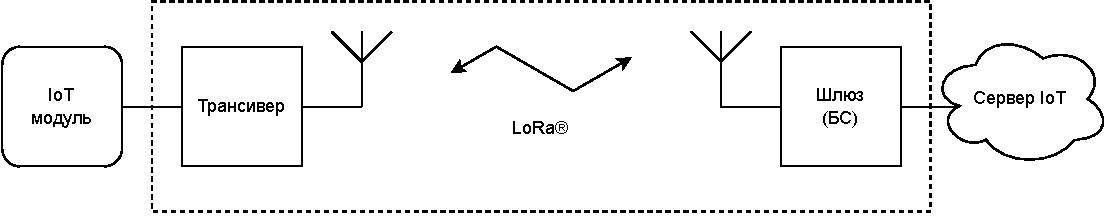
\includegraphics[width=0.9\textwidth,keepaspectratio]{SystemDraft.pdf}
	\caption{Структурная схема типичной системы связи для IoT}%
	\label{fig:SystemDraft}
\end{figure}

Необходимо разработать подсистему связи базовой станции (далее просто БС) и мобильное оконечное устройство (далее МОУ), использующие технологию LoRa. Для мобильного модуля также необходимо разработать компактную антенну. 

Все устройства системы должны удовлетворять стандарту RU864-870 и соответствовать требованиям, определяемых Приложением 11 к решению \linebreak ГКРЧ от 07.05.2007 №07-20-03-001:

\begin{longtblr}[
	caption = { Региональные стандарты, выдержка.},
	label = {table:regional-std}
	]{
		colspec={Q[223,l,m]Q[198,l,m]Q[429,l,m]},width=1.05\textwidth,
		vlines,hlines,
		vspan=even,
		rowhead=1,
		row{1}={font=\bfseries}
	}
	%%%%%%%%%%%%%%%%%%%%%%%%%%%%%%%%%%%%%%%%%%%%%%%
	Полоса радиочастот, МГц & Максимальная ЭИИМ, мВт &  Ограничения \\
	%%%%%%%%%%%%%%%%%%%%%%%%%%%%%%%%%%%%%%%%%%%%%%%%
	864 -- 865 		& 25 & Рабочий цикл 0,1\% или режим LBT \\
	868,7 -- 869,2 	& 25 & Рабочий цикл 0,1\% или режим LBT \\
\end{longtblr}

Средняя скорость передачи данных в сети должна быть не менее 1 кб/с

Основными требованиями к БС являются:
\begin{itemize}
	\setlength\itemsep{-1ex}
	\item Одновременная обработка данных от нескольких устройств
	\item Чувствительность не более минус 120 дБм
	\item Максимальная выходная мощность 12-14 дБм
\end{itemize}

Основными требованиями к МОУ являются:

\begin{itemize}
	\setlength\itemsep{-1ex}
	\item Возможность работы от аккумулятора или другого компактного источника питания
	\item Размеры (ДхШ) не более 6х6 см
	\item Чувствительность не более минус 120 дБмВт
	\item Максимальная выходная мощность 10-14 дБмВт
\end{itemize}

Основными требованиями к мобильной антенне являются всенаправленность и наибольший линейный размер в пределах 20 мм.



	\section{Разработка базовой станции.}
\subsection{Разработка структурной схемы.}
Определим основные составляющие элементы модуля БС. Монополистом в области производства чипов для базовых станций LoRa/LoRaWAN является компания Semtech. Из всего ассортимента продукции этой компании более всего нам подходят чип обработки данных SX1301, позволяющий обрабатывать данные от ~10000 оконечных устройств одновременно\cite{KimLee2020}, и приёмопередатчик SX1257, необходимый для работы в частотах, определяемых региональным стандартом.

На основании приведенных производителем макетных и примерных схем составим структурную схему БС. Отдельно поясним входную цепь: в рабочей полосе частот МШУ работает большое количество различных радиопередающих устройств с различной мощностью. Для избежания перехода усилителя в нелинейный режим работы и искажения принимаемого сигнала необходимо ограничить полосу принимаемых частот, для чего перед МШУ устанавливается ППФ. 

\begin{figure}[H]
	\centering
	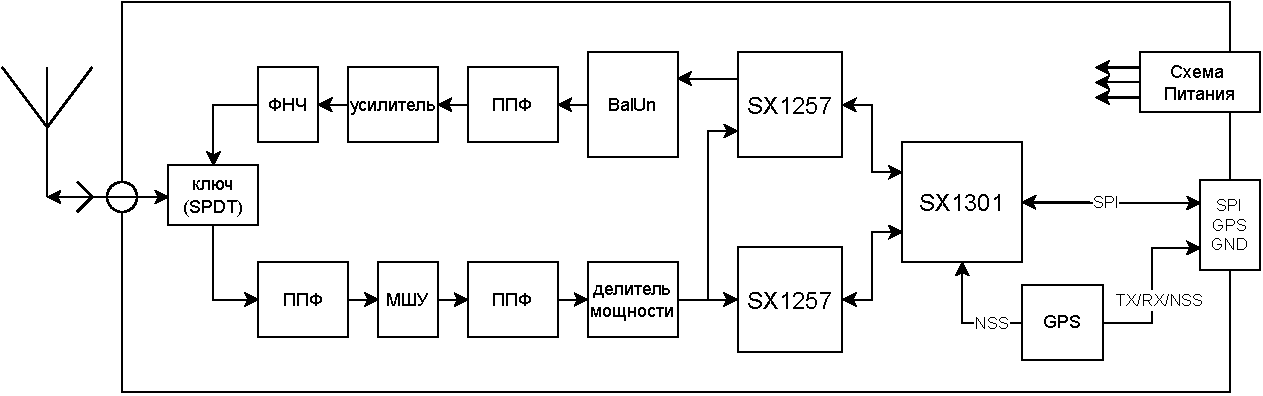
\includegraphics[width=0.9\textwidth,keepaspectratio]{BS-StructSch.pdf}
	\caption{Структурная схема БС}%
	\label{fig:BS-StructSch}
\end{figure}


\subsection{Выбор ЭКБ}
Исходя из составленной структурной схемы был произведён подбор электронной компонентной базы для БС.

\subsubsection{Выбор ППФ}

В диапазоне УКВ широкое распространение получили фильтры на поверхностных акустических волнах (ПАВ). Это обусловлено их высокими электрическими характеристиками (малые потери, малый коэффициент прямоугольности и высокая избирательность фильтра) при малых габаритных размерах. Кроме того, фильтры на ПАВ более устойчивы к внешним воздействующим факторам по сравнению с аналогами.

Исходя из стоимости, доступности, качества и количества предоставляемой производителем информации об устройстве, был выбран фильтр ФП3П7-814-10 производства Бутис-М. Производитель рекомендует его для применения в устройствах сетей LoRaWAN. Его размеры составляют 3х3х1,5 мм, а основные характеристики приведены на Рисунках \ref{fig:SAW-filter-graph-pass} и \ref{fig:SAW-filter-graph-VSWR}

\begin{figure}[H]
	\centering
	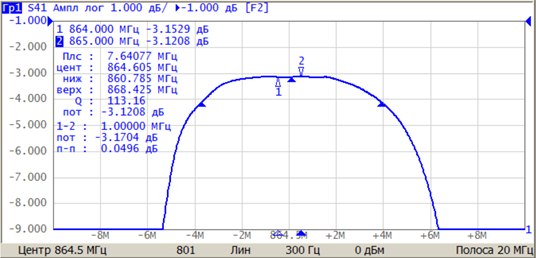
\includegraphics[width=0.8\textwidth,keepaspectratio]{SAW-filter-graph-pass.png}
	\caption{Передаточная характеристика фильтра ФП3П7-814-10}%
	\label{fig:SAW-filter-graph-pass}
\end{figure}

\begin{figure}[H]
	\centering
	\begin{subfigure}[b]{0.49\textwidth}
		\centering
		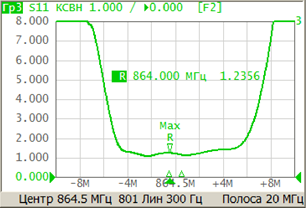
\includegraphics[width=\textwidth]{SAW-filter-graph-VSWR1.png}
		\caption{}%
		\label{fig:SAW-filter-graph-VSWR1}
	\end{subfigure}
	\hfill
	\begin{subfigure}[b]{0.49\textwidth}
		\centering
		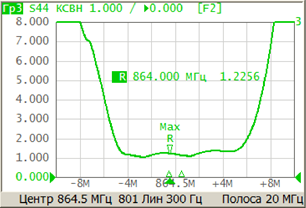
\includegraphics[width=\textwidth]{SAW-filter-graph-VSWR2.png}
		\caption{}%
		\label{fig:SAW-filter-graph-VSWR2}
	\end{subfigure}
	\caption{%
		КСВН фильтра ФП3П7-814-10
		(а) по входу и
		(б) по выходу 
	}%
	\label{fig:SAW-filter-graph-VSWR}
\end{figure}

\subsubsection{Выбор ФНЧ}
На роль ФНЧ был выбран фильтр 0868LP15A020 производства Johanson Technology. Его размеры составляют 2х1,25х1 мм, а основные характеристики приведены на Рисунке \ref{fig:LPF-graph}.

\begin{figure}[H]
	\centering
	\begin{subfigure}[b]{0.49\textwidth}
		\centering
		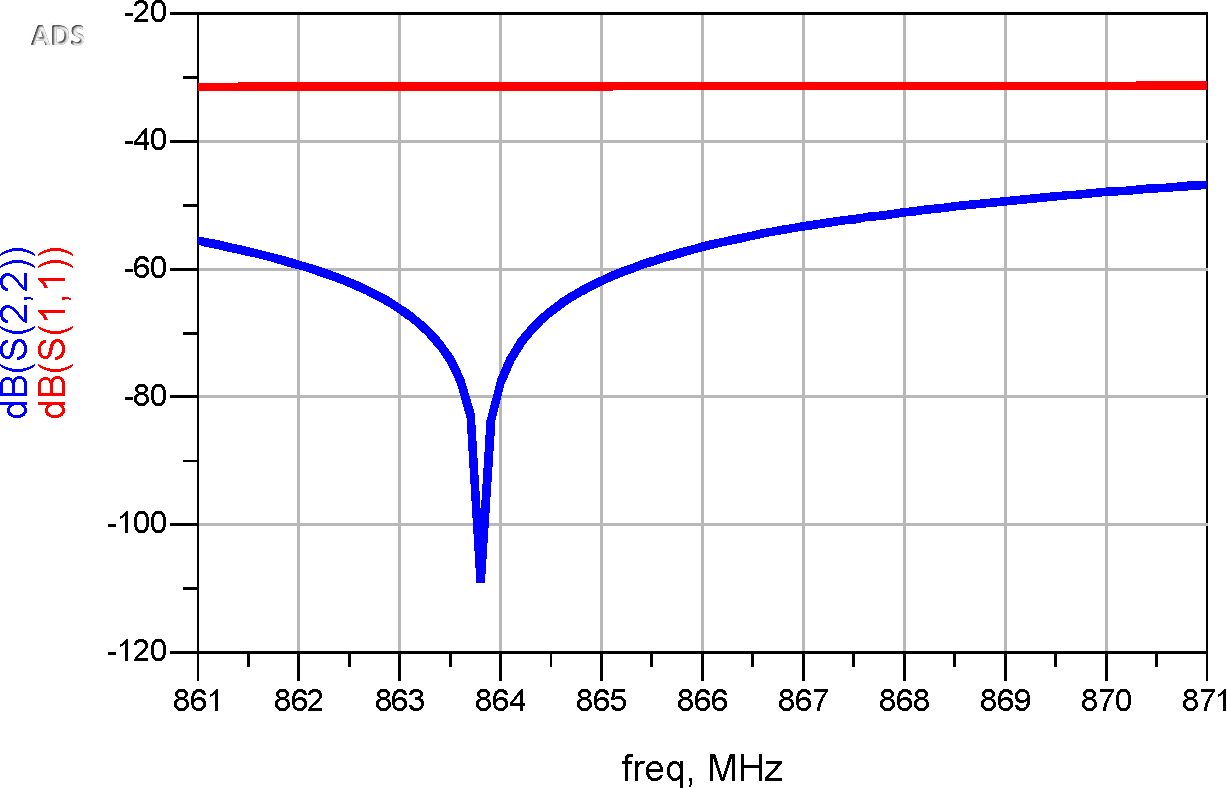
\includegraphics[width=\textwidth]{LPF-graph1122.pdf}
		\caption{}%
		\label{fig:LPF-graph1122}
	\end{subfigure}
	\hfill
	\begin{subfigure}[b]{0.49\textwidth}
		\centering
		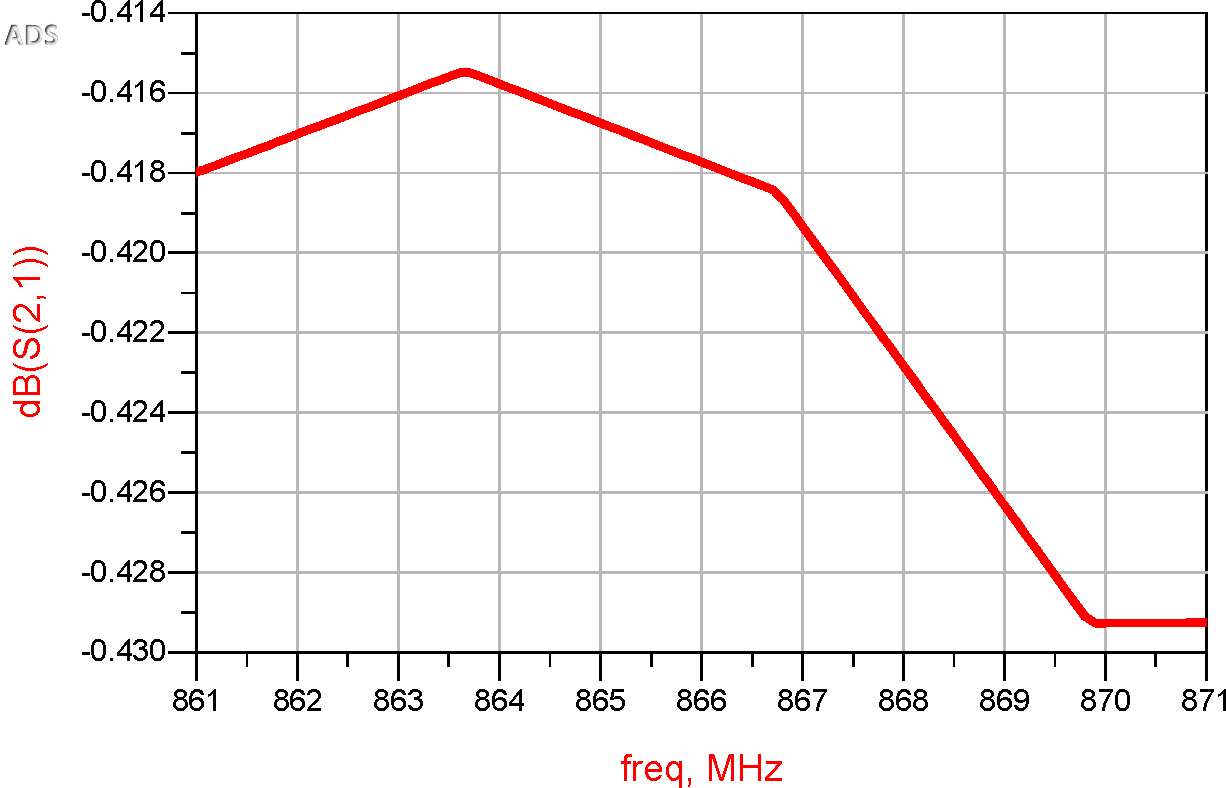
\includegraphics[width=\textwidth]{LPF-graph21.pdf}
		\caption{}%
		\label{fig:LPF-graph21}
	\end{subfigure}
	\caption{%
		КСВН фильтра ФП3П7-814-10
		(а) по входу и
		(б) по выходу 
	}%
	\label{fig:LPF-graph}
\end{figure}


\subsubsection{Выбор симметрирующего трансформатора}
В качестве симметрирующего трансформатора был выбран чип  \linebreak 0868BM15C0001 с размерами 2х1,25х1 мм. Его основные характеристики приведены на рисунках \ref{fig:balun-graph-SP} и \ref{fig:balun-graph-dirdif}.

\begin{figure}[H]
	\centering
	\begin{subfigure}[b]{0.49\textwidth}
		\centering
		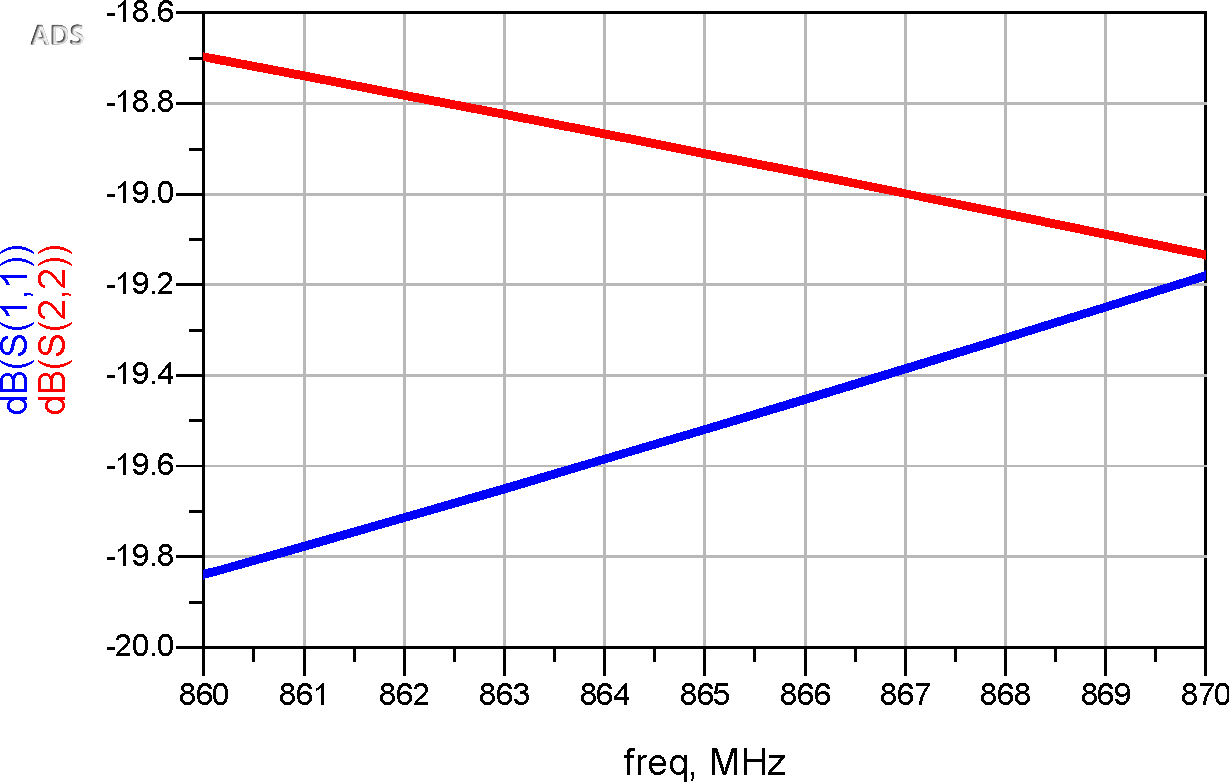
\includegraphics[width=\textwidth]{balun-graph-SP1122.pdf}
		\caption{}%
		\label{fig:balun-graph-SP1122}
	\end{subfigure}
	\hfill
	\begin{subfigure}[b]{0.49\textwidth}
		\centering
		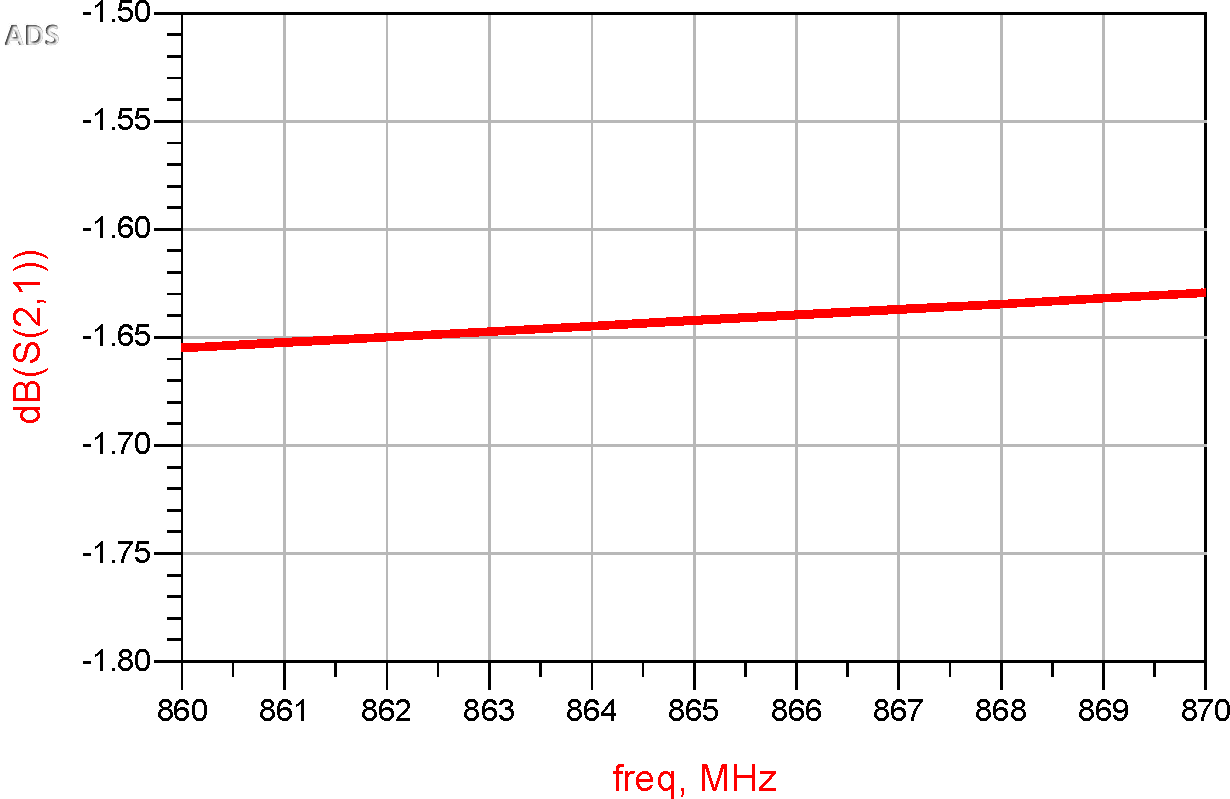
\includegraphics[width=\textwidth]{balun-graph-SP21.pdf}
		\caption{}%
		\label{fig:balun-graph-SP21}
	\end{subfigure}
	\caption{%
		Характеристики симметрирующего трансформатора 0868BM15C000
		(а) Коэффициенты отражения (дБ)
		(б) коэффициент передачи (дБ) 
	}%
	\label{fig:balun-graph-SP}
\end{figure}


\begin{figure}[H]
	\centering
	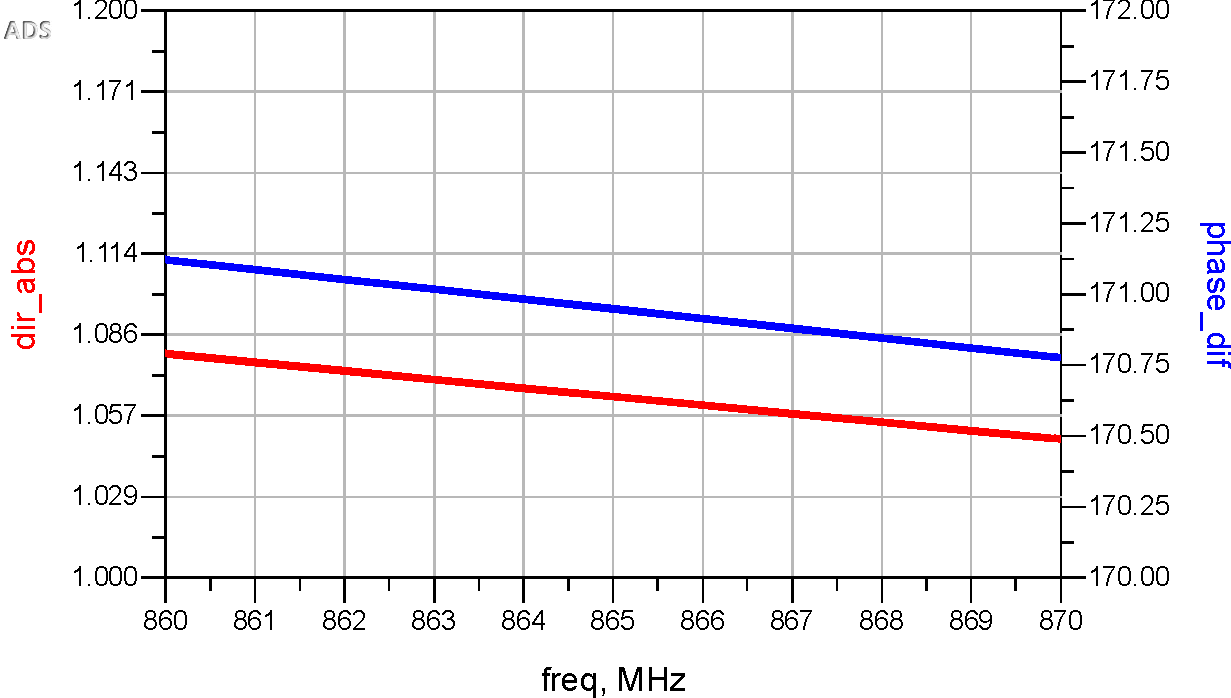
\includegraphics[width=0.8\textwidth,keepaspectratio]{balun-graph-dirdif.pdf}
	\caption{ Направленность (отношение амплитуд) и разница фаз балансных портов симметрирующего трансформатора 0868BM15C0001}%
	\label{fig:balun-graph-dirdif}
\end{figure}

\subsubsection{Выбор МШУ}

Для уменьшения коэффициента шума и улучшения чувствительности приёмного тракта требуется малошумящий усилитель. На его роль был выбран SPF5043Z производства Qorvo. Его основные параметры в необходимой полосе частот сведены в Таблице \ref{table:LNA-parameters}.

\begin{longtblr}[
	caption = {Основные параметры SPF5043Z},
	label = {table:LNA-parameters}
	]{
		colspec={Q[1,l,m]Q[1,l,m]},width=\textwidth,
		vlines,hlines,
		vspan=even,
		rowhead=1,
		row{1}={font=\bfseries}
	}
	%%%%%%%%%%%%%%%%%%%%%%%%%%%%%%%%%%%%%%%%%%%%%%%
	Параметр & Значение \\
	%%%%%%%%%%%%%%%%%%%%%%%%%%%%%%%%%%%%%%%%%%%%%%%%
	Усиление & 18,2 дБ \\
	Коэффициент шума & 0,7 дБ \\
	Точка однодецибельной компрессии & 22,6 дБмВт \\
	Размеры ШхДхВ & 2х2х1 мм \\
\end{longtblr}

\subsubsection{Выбор усилителя мощности}

Максимальная выходная мощность SX1257 равна -5 дБмВт. Для соответствия ТЗ требуется выходной усилитель мощности. Исходя из низкой стоимости, высокой эффективности и возможности регулирования усиления от 5 до 32 дБ был выбран усилитель RFPA0133 производства Qorvo. 

\subsubsection{Выбор опорных генераторов}

Для работы приемопередатчиков и процессора обработки данных требуются точные опорные генераторы. На их роль были выбраны KT2520K.32000. A.C.W.33.T.AS производства Kyocera и DSC1001CI2-133.0000 производства Microchip.

\subsubsection{Выбор ключа}

Выбираемый ключ должен иметь схему управления соответствующую SX1301, а именно - один управляющий сигнал выбирает рабочий порт, а другой разрешает или запрещает передачу сигнала. Данным параметрам соответствует RFSW1012. Его основные параметры показаны в таблице \ref{table:RFSW1012}

\begin{longtblr}[
	caption = {Основные gараметры выбранного ключа.},
	label = {table:RFSW1012}
	]{
		colspec={Q[1,l,m]Q[1,l,m]},width=\textwidth,
		vlines,hlines,
		vspan=even,
		rowhead=1,
		row{1}={font=\bfseries}
	}
	%%%%%%%%%%%%%%%%%%%%%%%%%%%%%%%%%%%%%%%%%%%%%%%
	Параметр & Значение \\
	%%%%%%%%%%%%%%%%%%%%%%%%%%%%%%%%%%%%%%%%%%%%%%%%
	Входные потери & 0,35 дБ \\
	Изоляция портов 1-2 & 48 дБ \\
	Диапазон частот & 5-6000 МГц \\
	Размеры (ШхДхВ) & 2х2х0,5 мм \\
\end{longtblr}

\subsubsection{Выбор GPS модуля.}

Для синхронизации времени и местоположения с сетью требуется информация о геолокации. Модуль uBlox Max7-Q имеет размеры (ШхДхВ) \linebreak 9,7х10,1х2,5 мм. Он поддерживает системы GPS и ГЛОНАСС, может определять местоположение с точностью до 2  м и имеет отдельный выход для генерации сигнала точного времени.

\subsection{Разработка подсистемы питания.}

Планируется питание от распространенных 9/12В блоков питания с штырьковым разъемом. В Таблице \ref{table:voltage-consumtion} показано потребление используемых устройств.

\begin{longtblr}[
	caption = {},
	label = {table:voltage-consumtion}
	]{
		colspec={Q[3,l,m]Q[4,l,m]Q[3,l,m]Q[6,l,m]},width=\textwidth,
		vlines,hlines,
		vspan=even,
		rowhead=1,
		row{1}={font=\bfseries}
	}
	%%%%%%%%%%%%%%%%%%%%%%%%%%%%%%%%%%%%%%%%%%%%%%%
	Устройство & Напряжение & Значение, В & Сила тока, макс, мА \\	
	%%%%%%%%%%%%%%%%%%%%%%%%%%%%%%%%%%%%%%%%%%%%%%%%
	\SetCell[r=2]{l} SX1301 
	& Питания портов & 3,3 & 10 \\
	& Питания ядра & 1,8 & 750 \\
	
	SX1257 & Питания & 3,3 & 85 \\
	
	VCXO & Питания & 3,3 & 2 \\
	
	\SetCell[r=2]{l} RFPA0133
	
	& Питания 1,2 & 3,6 & 250 \\
	& Смещения & 3 & 0,2 \\
	 
	SPF5043 & Питания & 5 & 100 \\
	
	RFSW1012 & Питания & 2,7-5,5 & 0,2 \\
	
	MAX7-Q & Питания & 3,3 & 67 \\	
\end{longtblr}

Формирование напряжения питания обеспечивается импульсными и линейными стабилизаторами напряжения. Первые нужны для высокоэффективного понижения напряжения, а вторые для устранения помех, создаваемыми в процессе их работы. На рисунке \ref{fig:BS-PowerSch} показана структурная схема подсистемы питания

\begin{figure}[H]
	\centering
	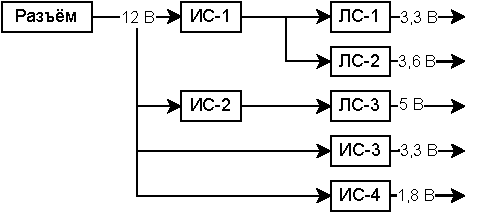
\includegraphics[width=0.8\textwidth,keepaspectratio]{BS-PowerSch.pdf}
	\caption{Структурная схема подсистемы питания БС}%
	\label{fig:BS-PowerSch}
\end{figure}

\begin{itemize}
	\item Разъём выберем DS-201 – это штырьковый разъём-розетка 2,1х5,5мм
	\item В качестве импульсных стабилизаторов будет применяться ST1S14PH производства STMicroelectronics – это стабилизатор с диапазоном входных напряжений от 5.5 до 48 В и выходным током до 3 А. Выходное напряжение регулируется с помощью резистивного делителя, рассчитываемого по формуле 
	\begin{equation}
		\label{eq:stab-voltage-output}
		V_{out}=1,22\cdot(1+R1/R2)
	\end{equation}
	Схема включения изображена на рисунке \ref{fig:ST1S14PH-PS}
	\begin{figure}[H]
		\centering
		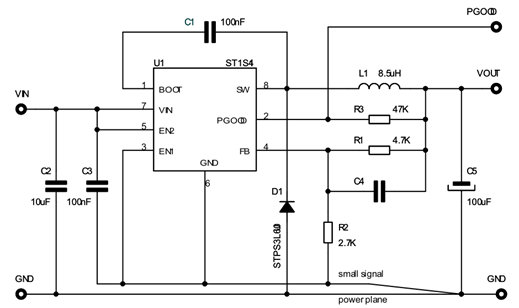
\includegraphics[width=0.8\textwidth,keepaspectratio]{ST1S14PH-PS.png}
		\caption{Типичная схема включения ST1S14PH}%
		\label{fig:ST1S14PH-PS}
	\end{figure}
	
	\item На роль линейных стабилизаторов был выбран LT1965EDD – это стабилизатор с диапазоном входных напряжений от 1,8 до 20 В, максимальным выходным током 1,1 А и падением напряжения 310 мВ. Выходное напряжение регулируется с помощью резистивного делителя, рассчитываемого по формуле \ref{eq:stab-voltage-output}.

	Схема включения изображена на рисунке \ref{fig:LT1965EDD-PS}.

	\begin{figure}[H]
		\centering
		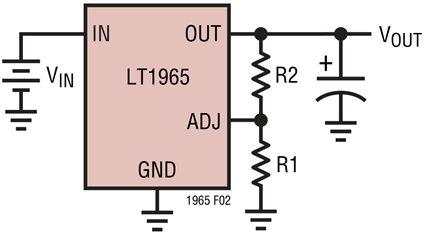
\includegraphics[width=0.8\textwidth,keepaspectratio]{LT1965EDD-PS.png}
		\caption{Типичная схема включения LT1965EDD-PS}%
		\label{fig:LT1965EDD-PS}
	\end{figure}
\end{itemize}

\subsection{Системное моделирование.}
Выполним моделирование каждого компонента по отдельности, а также входной и выходной цепи.

Моделирование каждого элемента выполняется поочередно в двух режимах – схемном и симуляционном. В первом для расчётов используются идеальные линии передачи, во втором строится  участок платы, включающий посадочное место устройства, сигнальные линии и линии питания, а также необходимые схемы согласования, и проводится моделирование с помощью ЕМ-симулятора.

Для уменьшения размеров устройства каждый блок будет согласован не с 50-тиомной линией, а с соседним блоком, таким образом моделирование цепи будет выполняться следующим образом: вход первого устройства согласуется с 50-тиомной линией, а сопротивление выходного порта приравнивается к выходному сопротивлению устройства, сопротивление входного порта следующего блока приравнивается к выходному сопротивлению предыдущего и согласуется с входным сопротивлением устройства; последний же блок согласуется по входу с предыдущим блоком, а по выходу - с 50-тиомной линией.

Рассчитаем общую для всего устройства ширину 50-тиомной линии с помощью утилиты TxLine. Параметры платы и линий будут задаваться с учётом технологических возможностей современных производств.

\begin{figure}[H]
	\centering
	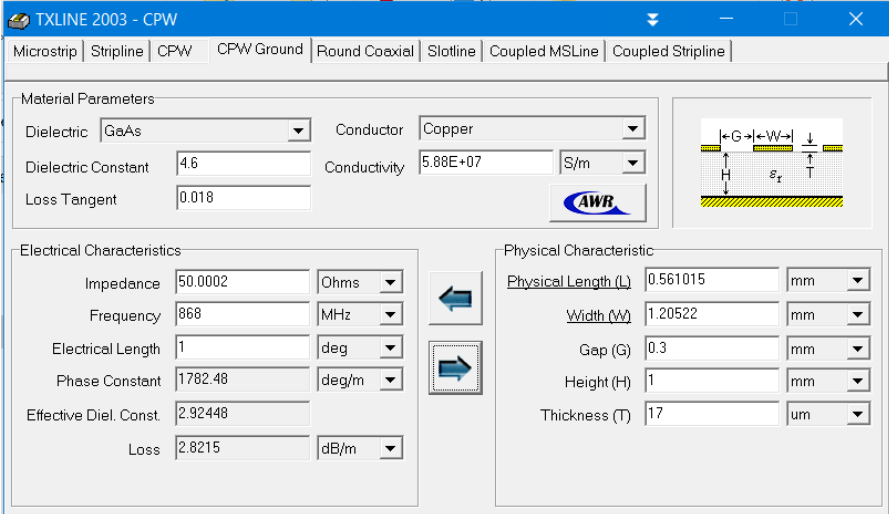
\includegraphics[width=0.8\textwidth,keepaspectratio]{BS LineCalc.png}
	\caption{Расчёт ширины линии}%
	\label{fig:BS LineCalc}
\end{figure}

\subsubsection{Результаты моделирования передающего тракта.}
На Рисунке \ref{fig:OPL-sch} показано схемное представление передающего тракта БС. Каждый блок был согласован и промоделирован с помощью ЕМ-симулятора. Результаты моделирования всего тракта показаны на Рисунках \ref{fig:OPL-imp} и \ref{fig:OPL-VSWR-trans}.

\begin{figure}[H]
	\centering
	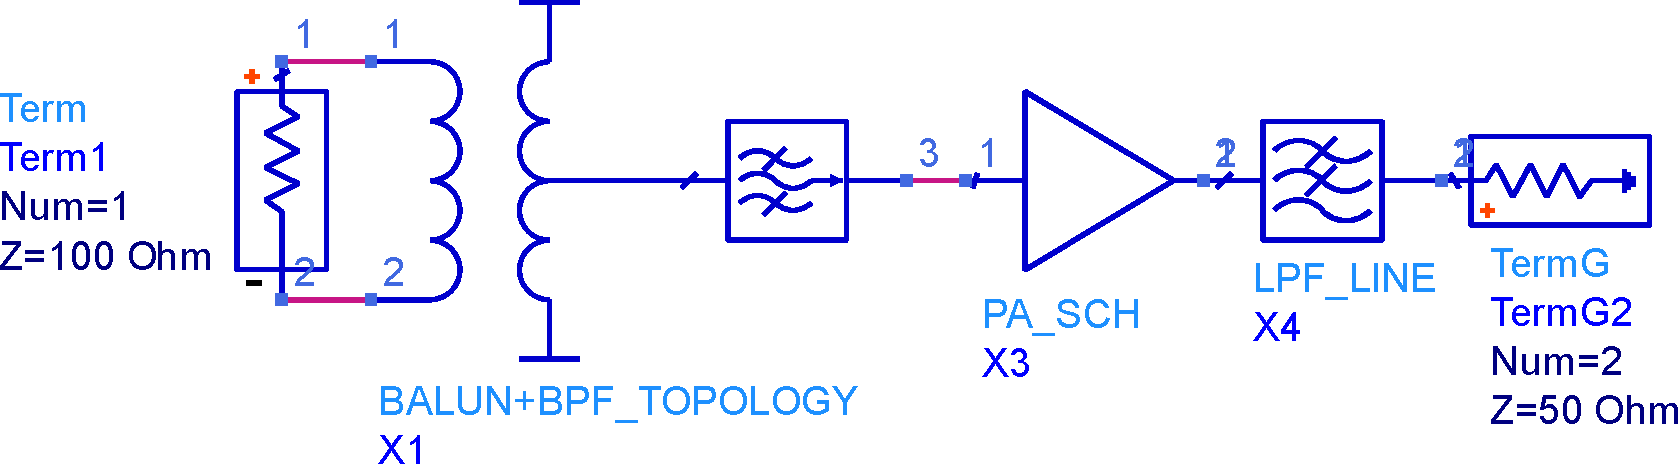
\includegraphics[width=\textwidth,keepaspectratio]{OPL-sch.pdf}
	\caption{Итоговая модель выходного тракта БС}%
	\label{fig:OPL-sch}
\end{figure}

\begin{figure}[H]
	\centering
	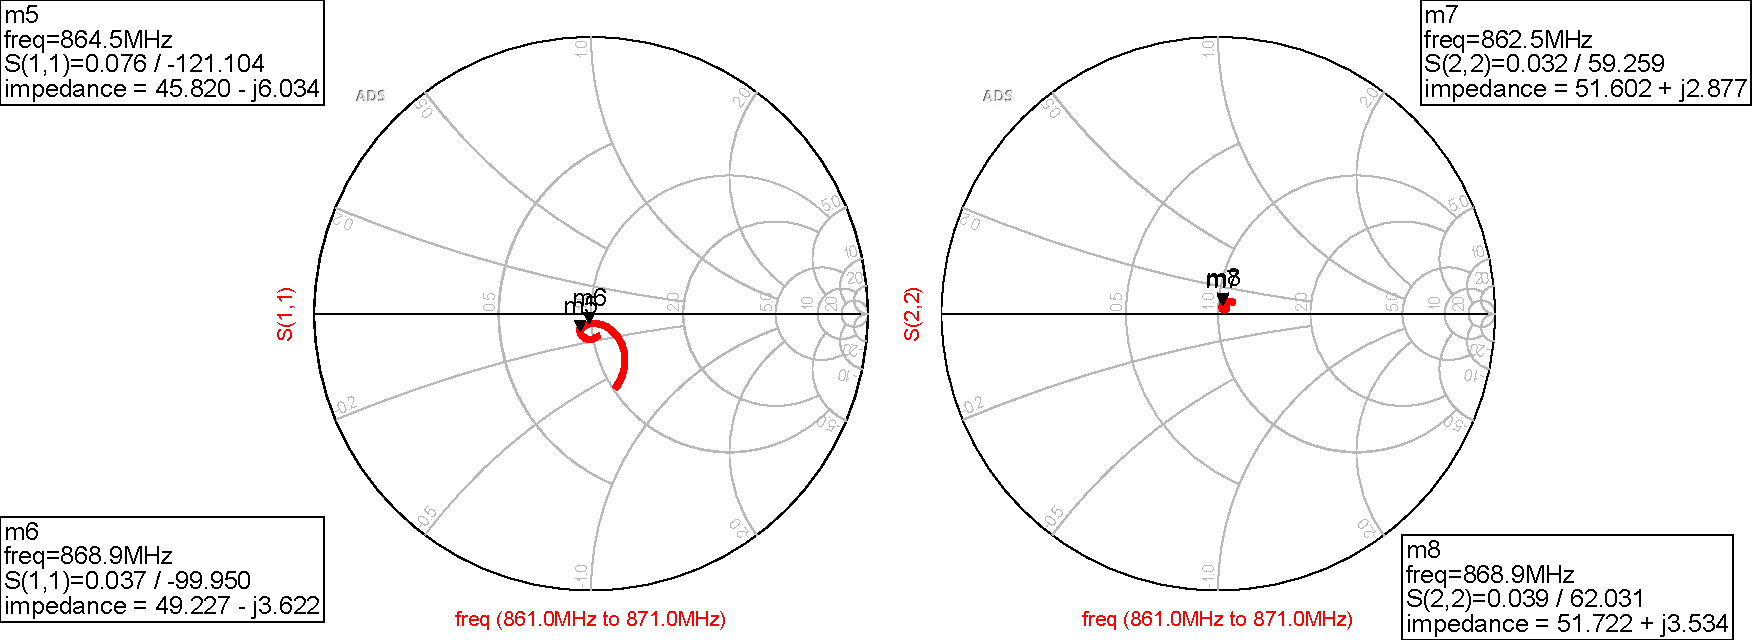
\includegraphics[width=\textwidth,keepaspectratio]{OPL-imp.pdf}
	\caption{входное и выходное сопротивление передающего тракта}%
	\label{fig:OPL-imp}
\end{figure}

\begin{figure}[H]
	\centering
	\begin{subfigure}[b]{0.49\textwidth}
		\centering
		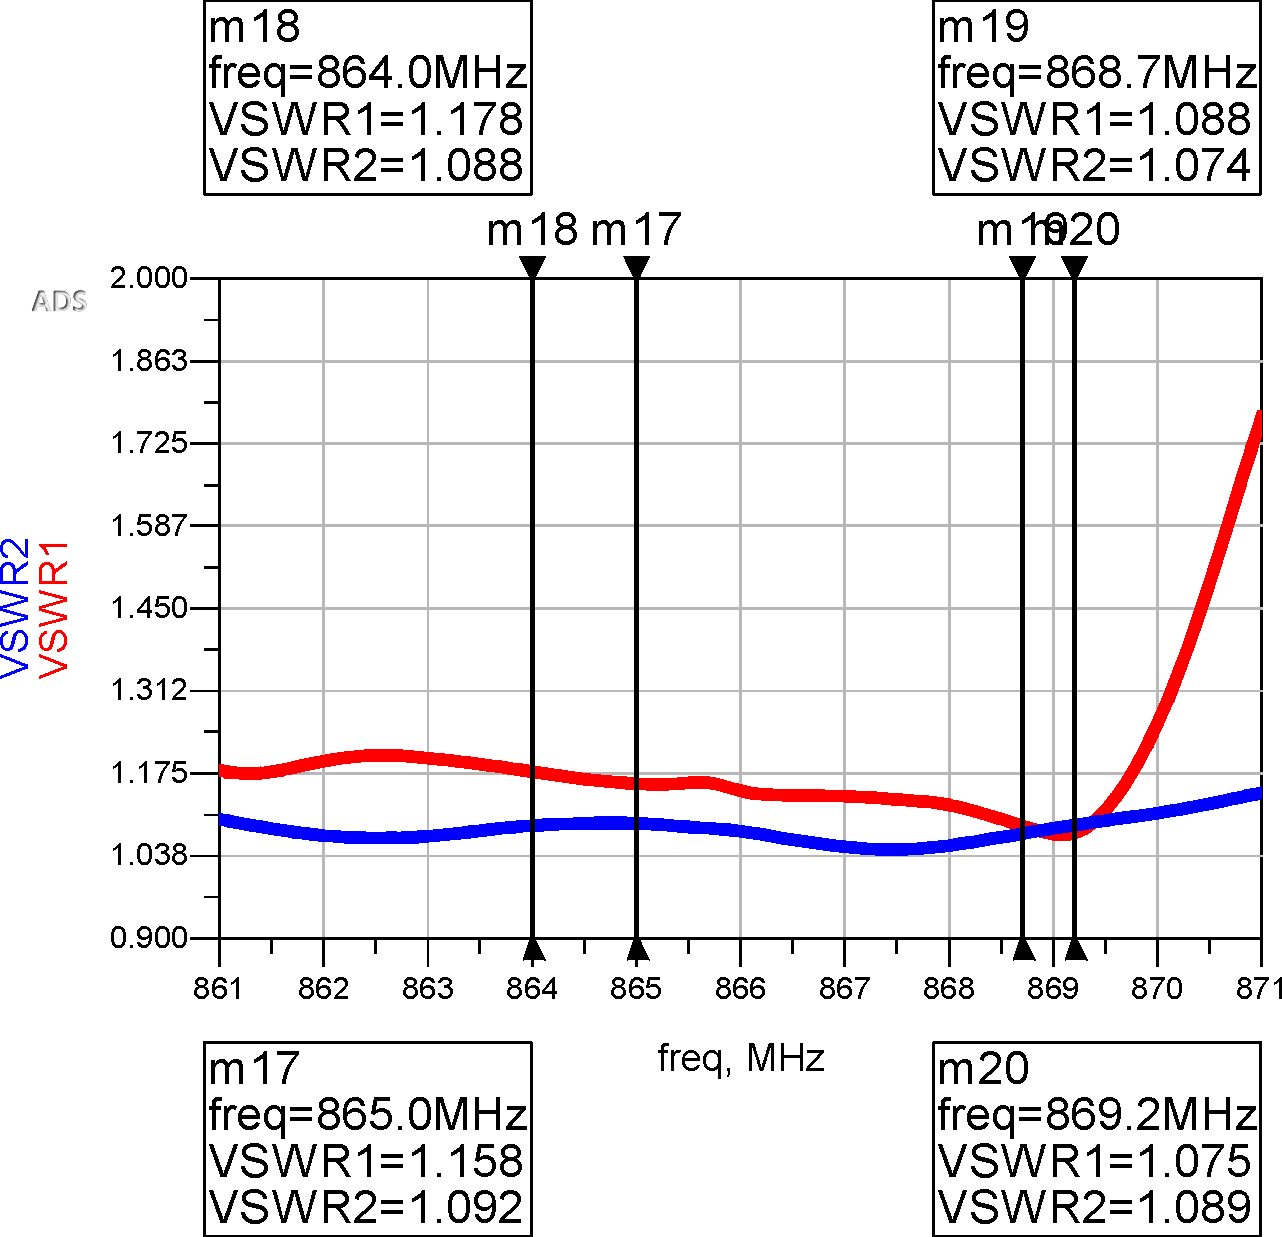
\includegraphics[width=\textwidth]{OPL-VSWR.pdf}
		\caption{}%
		\label{fig:OPL-VSWR}
	\end{subfigure}
	\hfill
	\begin{subfigure}[b]{0.49\textwidth}
		\centering
		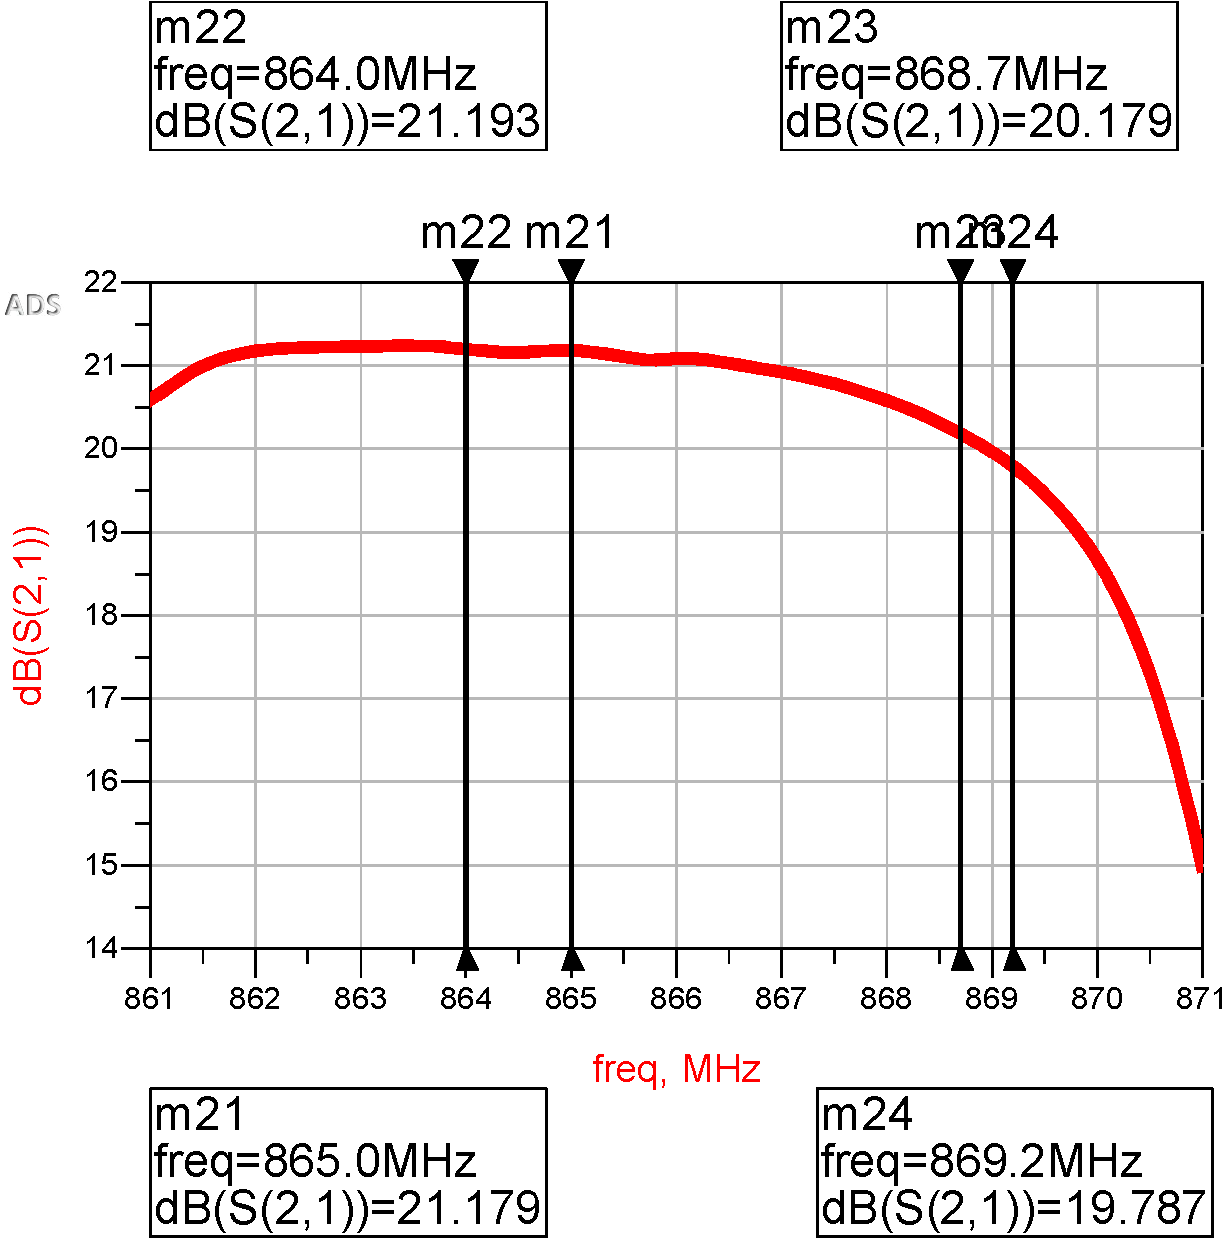
\includegraphics[width=\textwidth]{OPL-trans.pdf}
		\caption{}%
		\label{fig:OPL-trans}
	\end{subfigure}
	\caption{%
		(а) КСВН передающего тракта
		(б) Коэффициент передачи передающего тракта (дБ)
	}%
	\label{fig:OPL-VSWR-trans}
\end{figure}

На рисунке \ref{fig:OPL-trans} показано максимально возможное усиление в канале. Максимальная выходная мощность SX1257 равна -5 дБм, таким образом максимально возможная выходная мощность равна 16 дБм. С помощью программного регулирования можно устанавливать выходную мощность от  -7 до 16 дБм, таким образом требование к мощности передаваемого сигнала можно считать удовлетворенным.

Стоит, однако, отметить, что производитель выходного усилителя не предоставил файлов S-параметров, поэтому для моделирования использовался универсальный блок усилителя, параметры которого задавались исходя из имеющейся документации на элемент. Для более точного определения параметров элемента и более качественного его согласования была разработана измерительная плата, а для ускорения процесса производства на плате основного устройства будут размещены посадочные места для универсальной схемы согласования. Подробнее про разработку платы измерения параметров УМ рассказано в Главе \ref{sect:bs-oa-mes}.

\subsubsection{Результаты моделирования приемного тракта.}
Основной участок приёмного тракта необходимо спроектировать так, чтобы с одной стороны он был согласован с антенной, а с другой - с делителем мощности.

На Рисунке \ref{fig:IPL-sch} показано схемное представление передающего тракта БС. Каждый блок был согласован и промоделирован с помощью ЕМ-симулятора. Результаты моделирования всего тракта показаны на Рисунках \ref{fig:IPL-imp}, \ref{fig:IPL-VSWR-trans} и \ref{fig:IPL-NF}.

\begin{figure}[H]
	\centering
	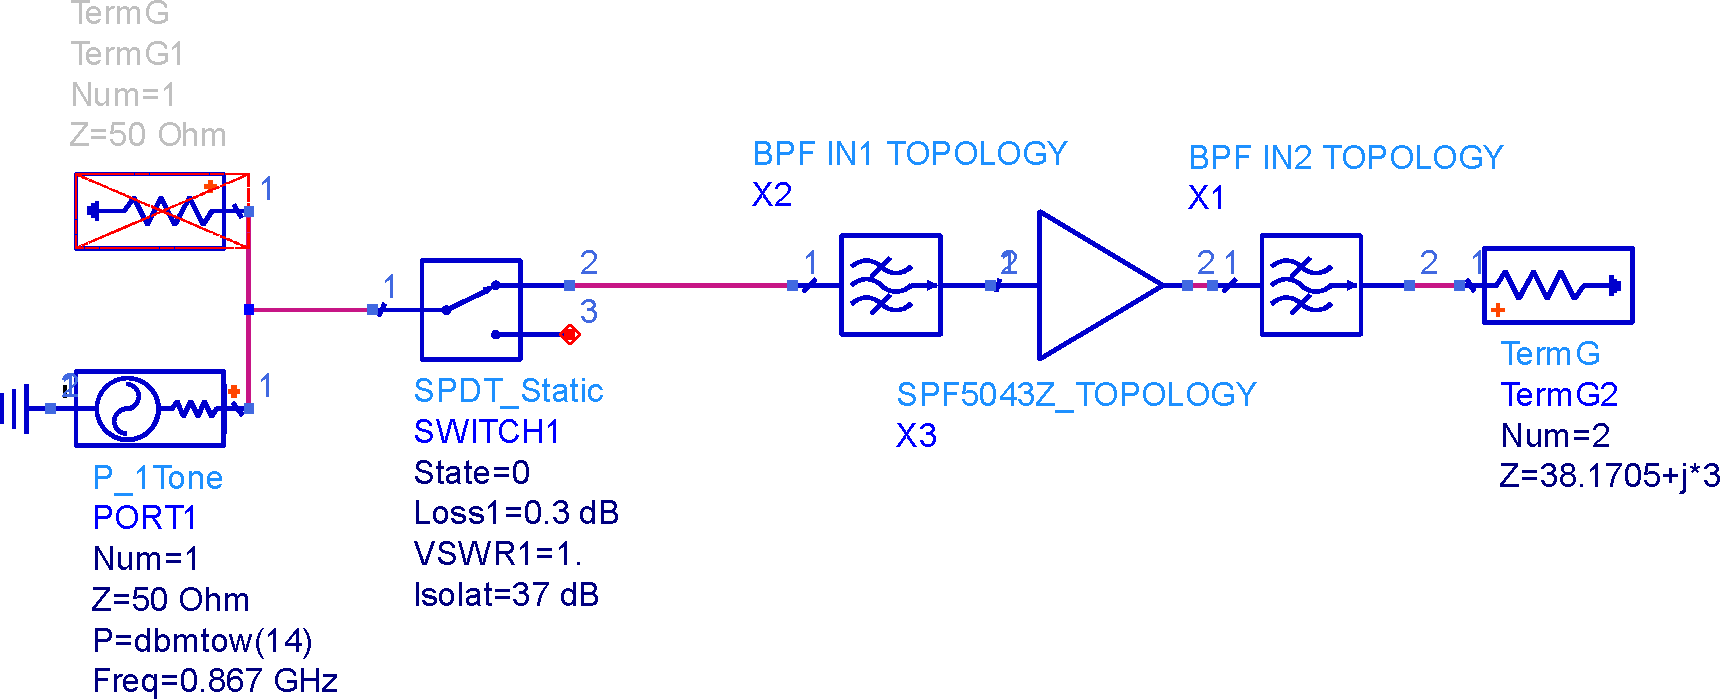
\includegraphics[width=\textwidth,keepaspectratio]{IPL-sch.pdf}
	\caption{Итоговая модель приемного тракта БС}%
	\label{fig:IPL-sch}
\end{figure}

\begin{figure}[H]
	\centering
	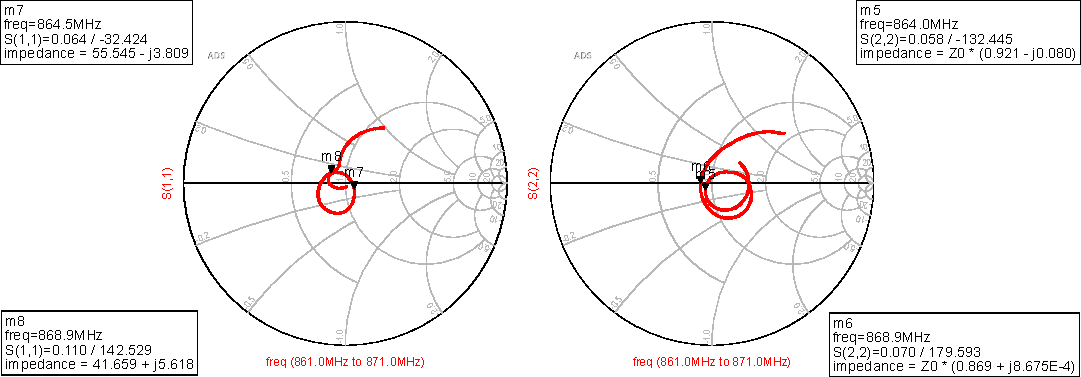
\includegraphics[width=0.9\textwidth,keepaspectratio]{IPL-imp.pdf}
	\caption{входное и выходное сопротивление приёмного тракта}%
	\label{fig:IPL-imp}
\end{figure}

\begin{figure}[H]
	\centering
	\begin{subfigure}[b]{0.49\textwidth}
		\centering
		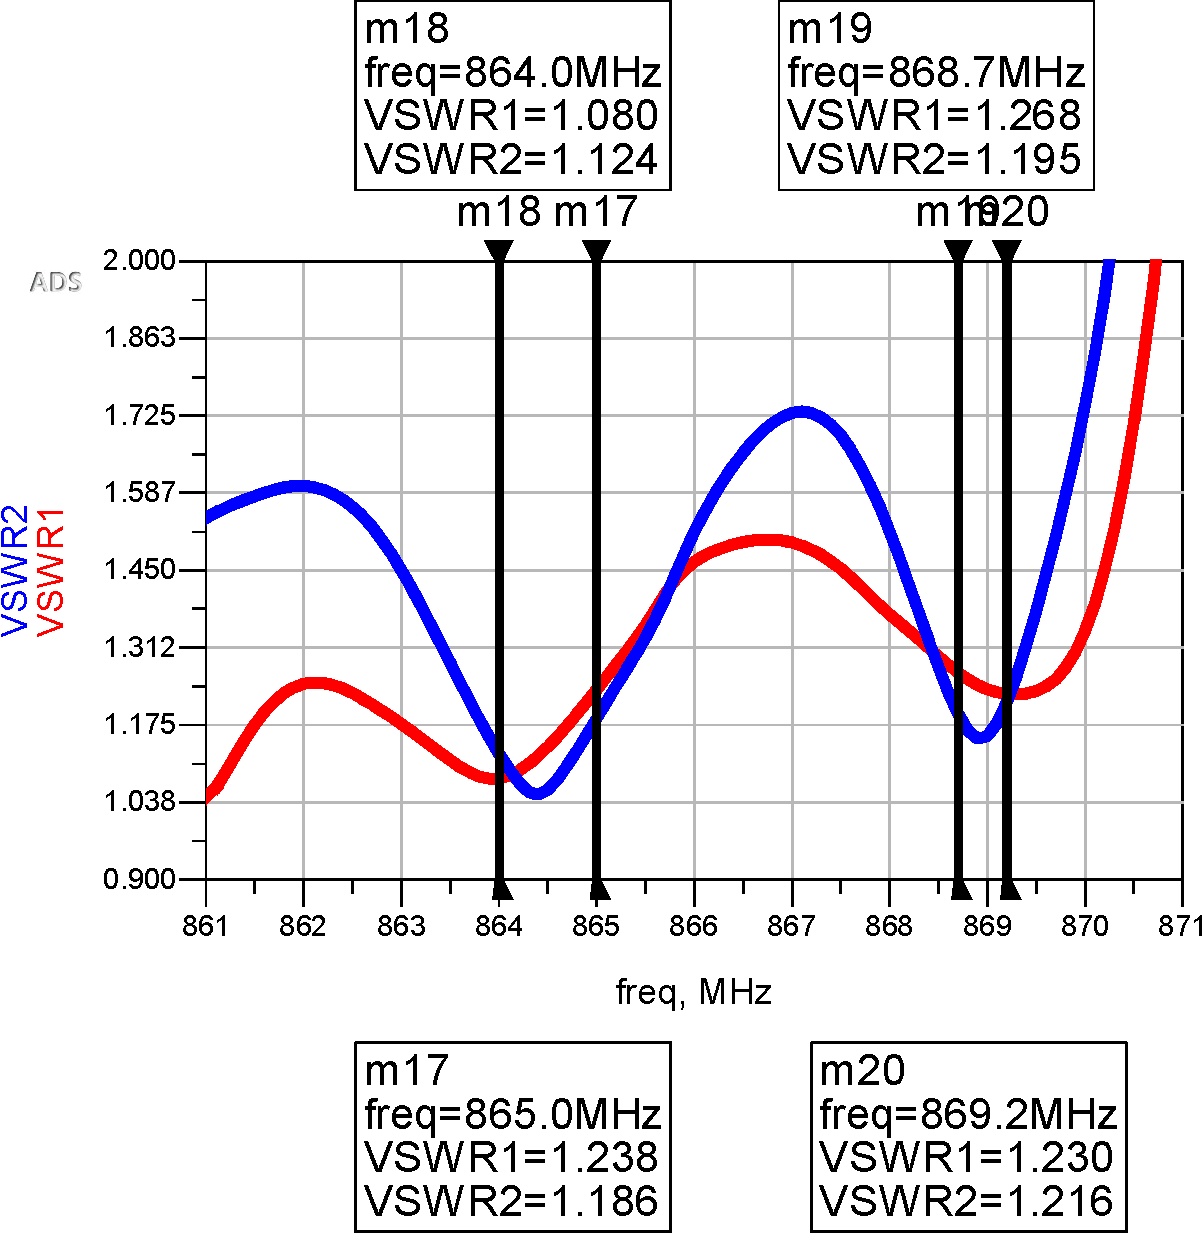
\includegraphics[width=\textwidth]{IPL-VSWR.pdf}
		\caption{}%
		\label{fig:IPL-VSWR}
	\end{subfigure}
	\hfill
	\begin{subfigure}[b]{0.49\textwidth}
		\centering
		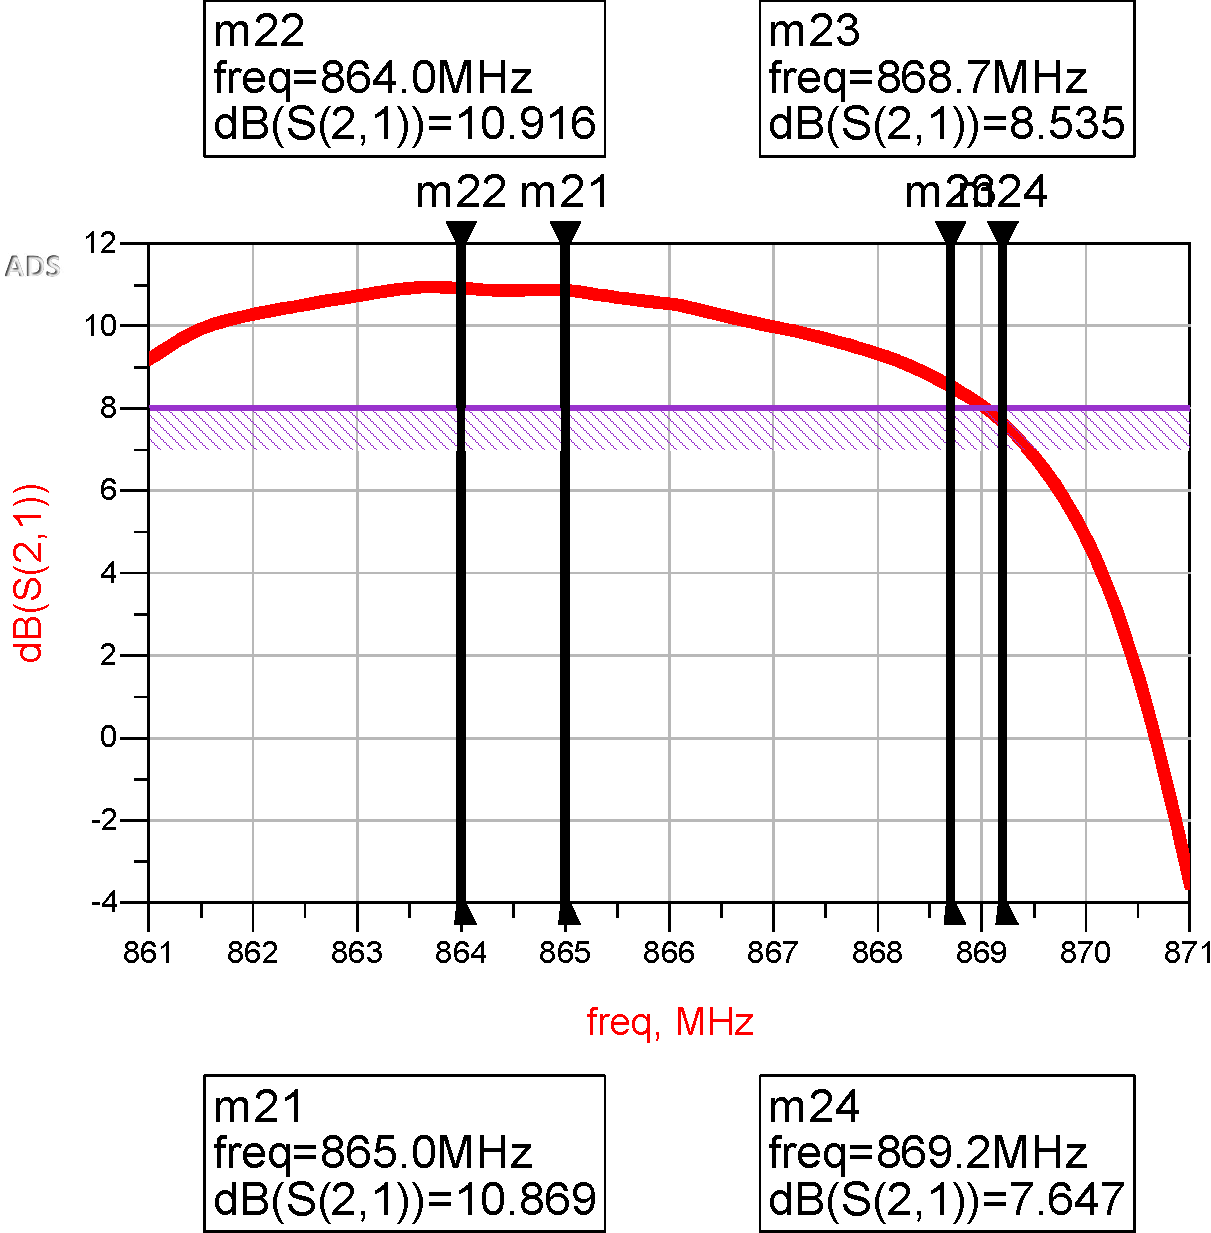
\includegraphics[width=\textwidth]{IPL-trans.pdf}
		\caption{}%
		\label{fig:IPL-trans}
	\end{subfigure}
	\caption{%
		(а) КСВН приёмного тракта
		(б) Коэффициент передачи приёмного тракта (дБ)
	}%
	\label{fig:IPL-VSWR-trans}
\end{figure}

\begin{figure}[H]
	\centering
	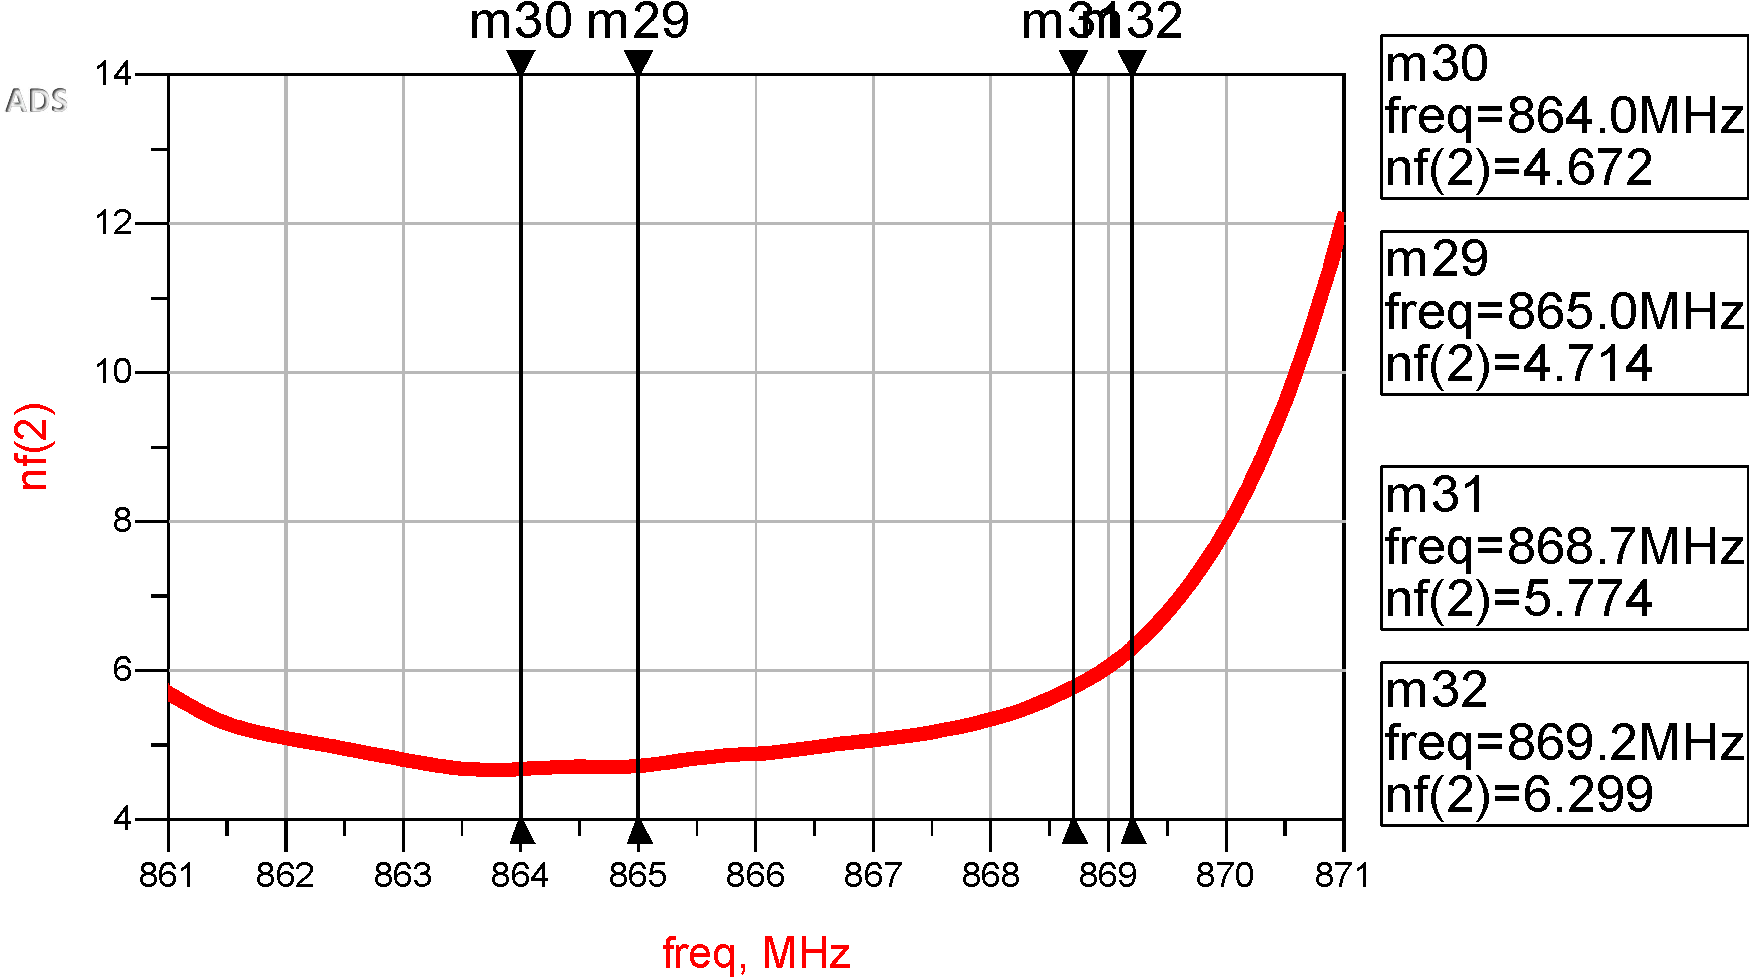
\includegraphics[width=0.75\textwidth,keepaspectratio]{IPL-NF.pdf}
	\caption{$K_\text{Ш}$ приемного тракта}%
	\label{fig:IPL-NF}
\end{figure}

Основываясь на полученных результатах произведем расчёт чувствительности устройства по формуле
\begin{equation}
	{Sensitivity}[\text{дБм}] = N[\text{дБм}]+{SNR}_\text{треб}[\text{дБ}]+NF-K_\text{п}+3
\end{equation}

Здесь N - мощность шума в выбранной полосе в дБм, ${SNR}_\text{треб}$ - требуемое отношение сигнал-шум в дБ, NF - коэффициент шума, $K_\text{п}$ - коэффициент передачи приемного тракта, дБ. 3 дБ необходимо прибавлять для учета деления мощности между приемопередатчиками. 

Расчёт чувствительности проводился для $f_c=869$~МГц, так как это позволяет оценить предельные возможности приемного тракта. Худшие показатели чувствительности достигаются при SF=6 и полосе 250~кГц. Требуемое отношение сигнал-шум в таком случае составляет -7.5 дБ. 
Экспортируем значения в переменные и рассчитаем чувствительность прямо в ADS. Расчёты и их результат показаны на Рисунке \ref{fig:IPL-sens-count}

\begin{figure}[H]
	\centering
	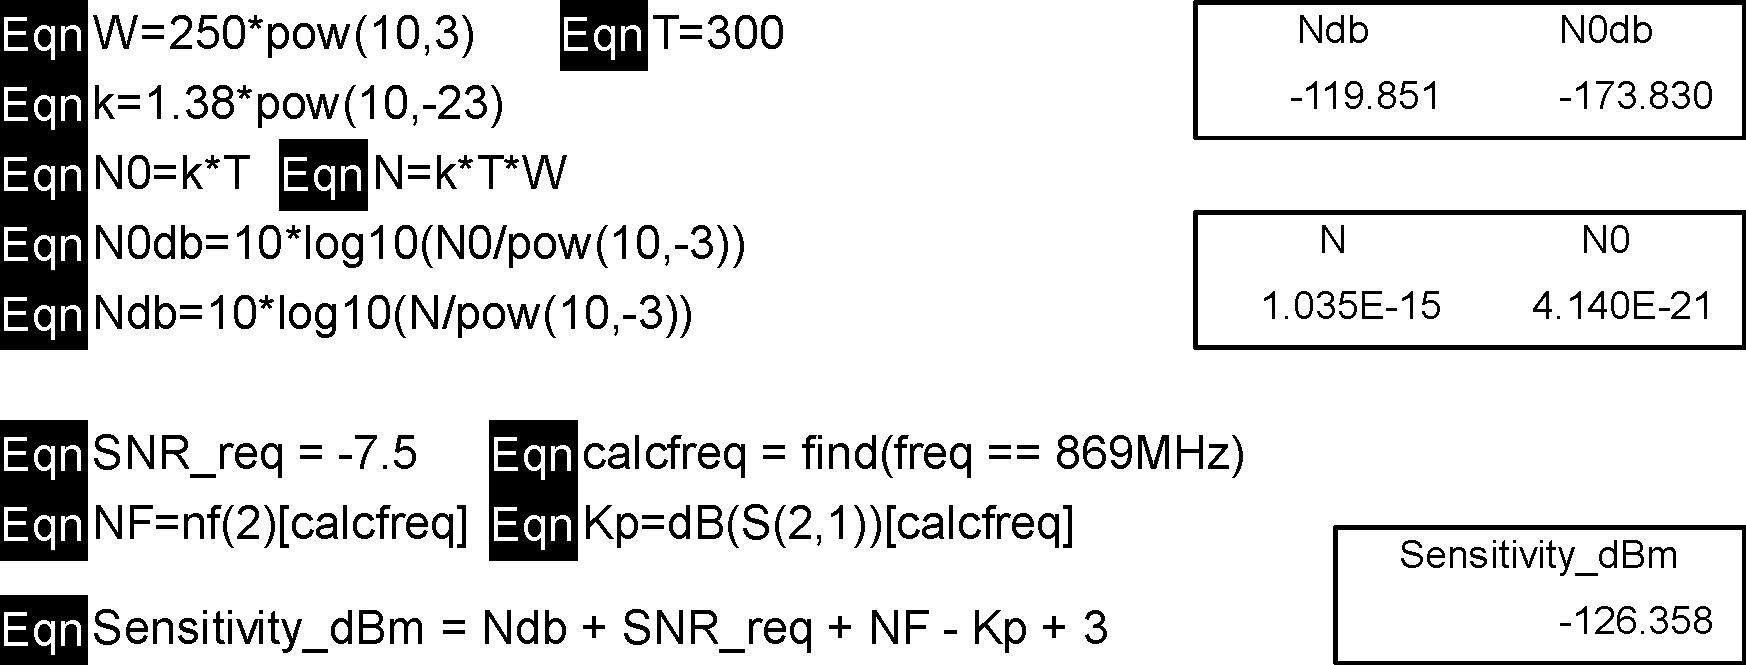
\includegraphics[width=\textwidth,keepaspectratio]{IPL-sens-count.pdf}
	\caption{Расчёт чувствительности приемного тракта БС}%
	\label{fig:IPL-sens-count}
\end{figure}

Рассчитанное значение чувствительности составляет минус 126 дБм, следовательно, ТЗ на приёмный тракт можно считать выполненным.

\subsubsection{Делитель мощности.}

Для увеличения возможностей параллельной многоканальной обработки данных необходимо разделять входной поток между двумя приемопередатчиками. Входное сопротивление SX1257 равно 50 Ом. Необходимо разработать и согласовать делитель мощности. На Рисунках \ref{fig:coupler-em} и \ref{fig:coupler-match} показаны топология и схема согласования делителя. 

\begin{figure}[H]
	\centering
	\begin{subfigure}[c]{0.49\textwidth}
		\centering
		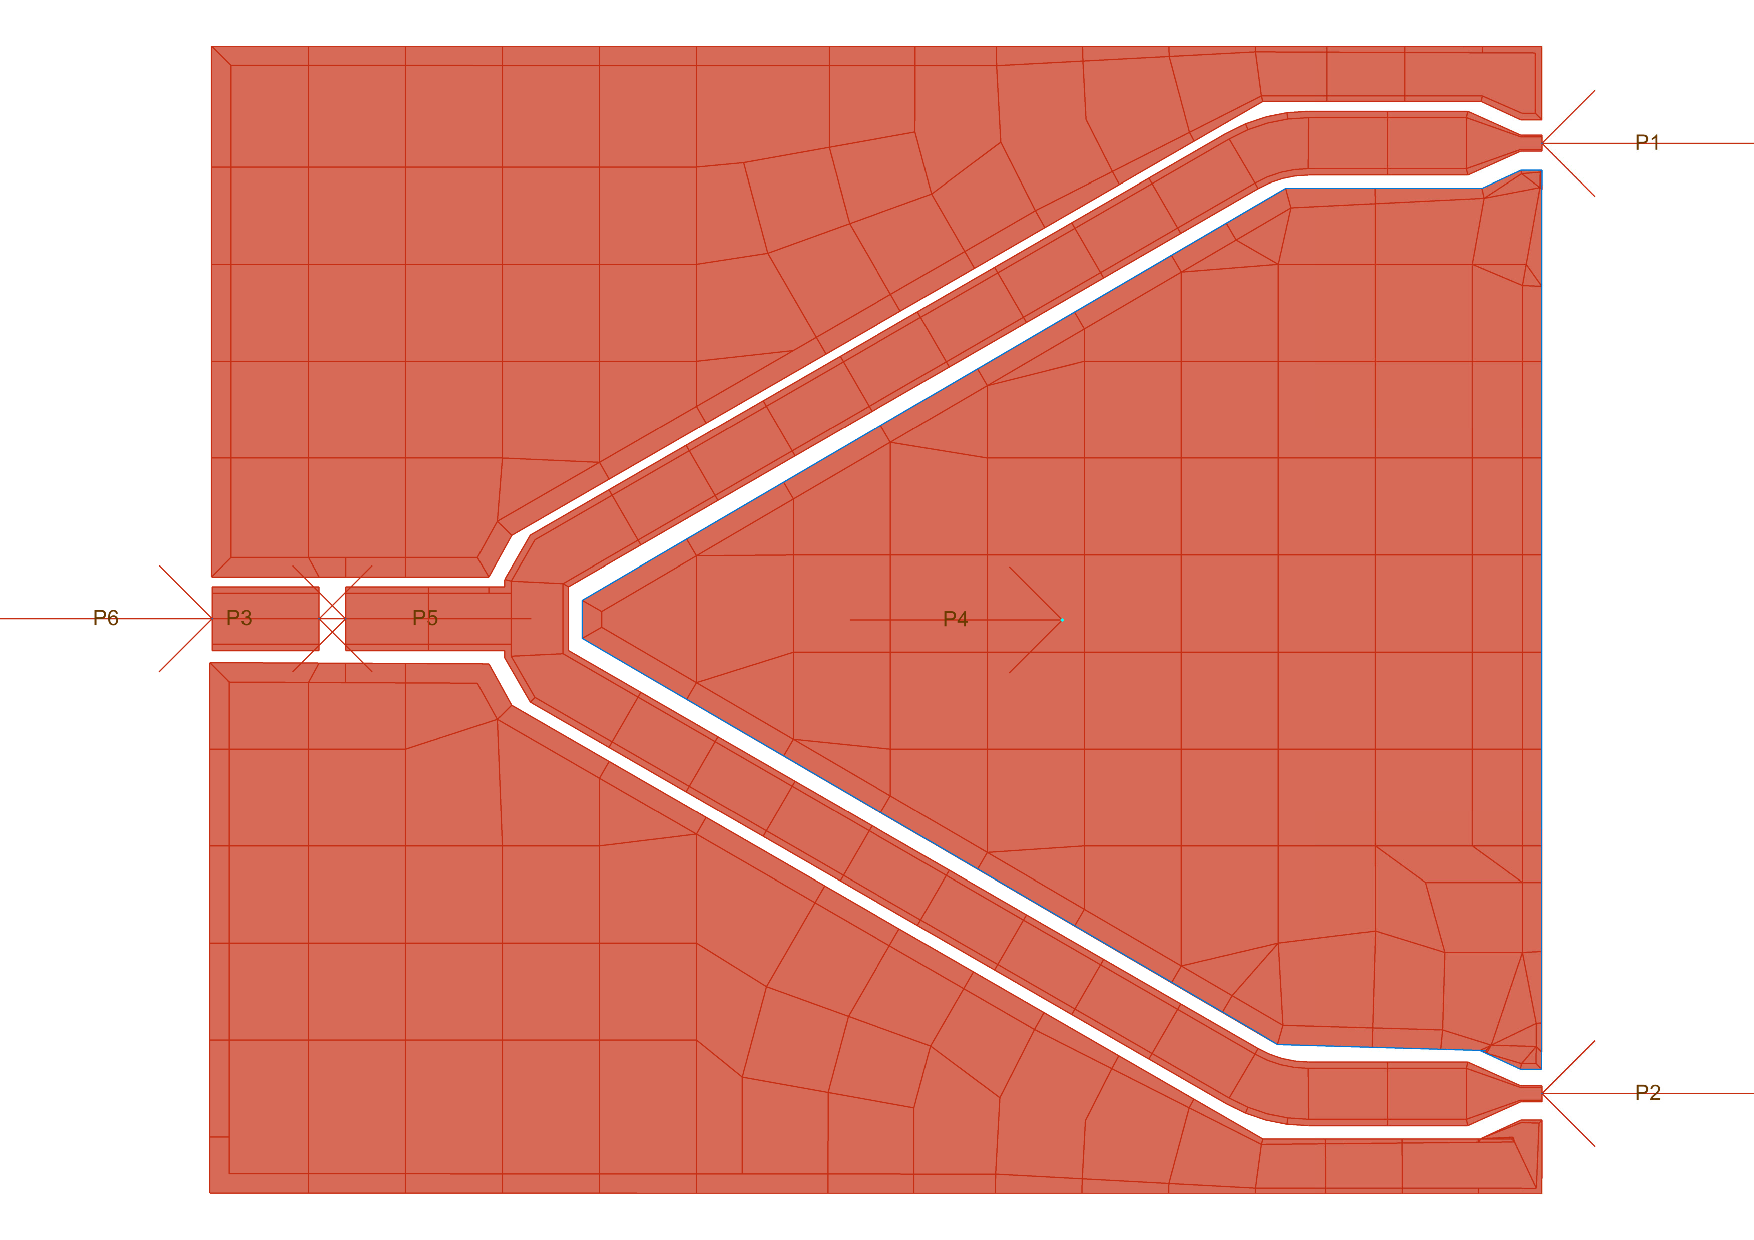
\includegraphics[width=\textwidth]{coupler-em.pdf}
		\caption{}%
		\label{fig:coupler-em}
	\end{subfigure}
	\hfill
	\begin{subfigure}[c]{0.49\textwidth}
		\centering
		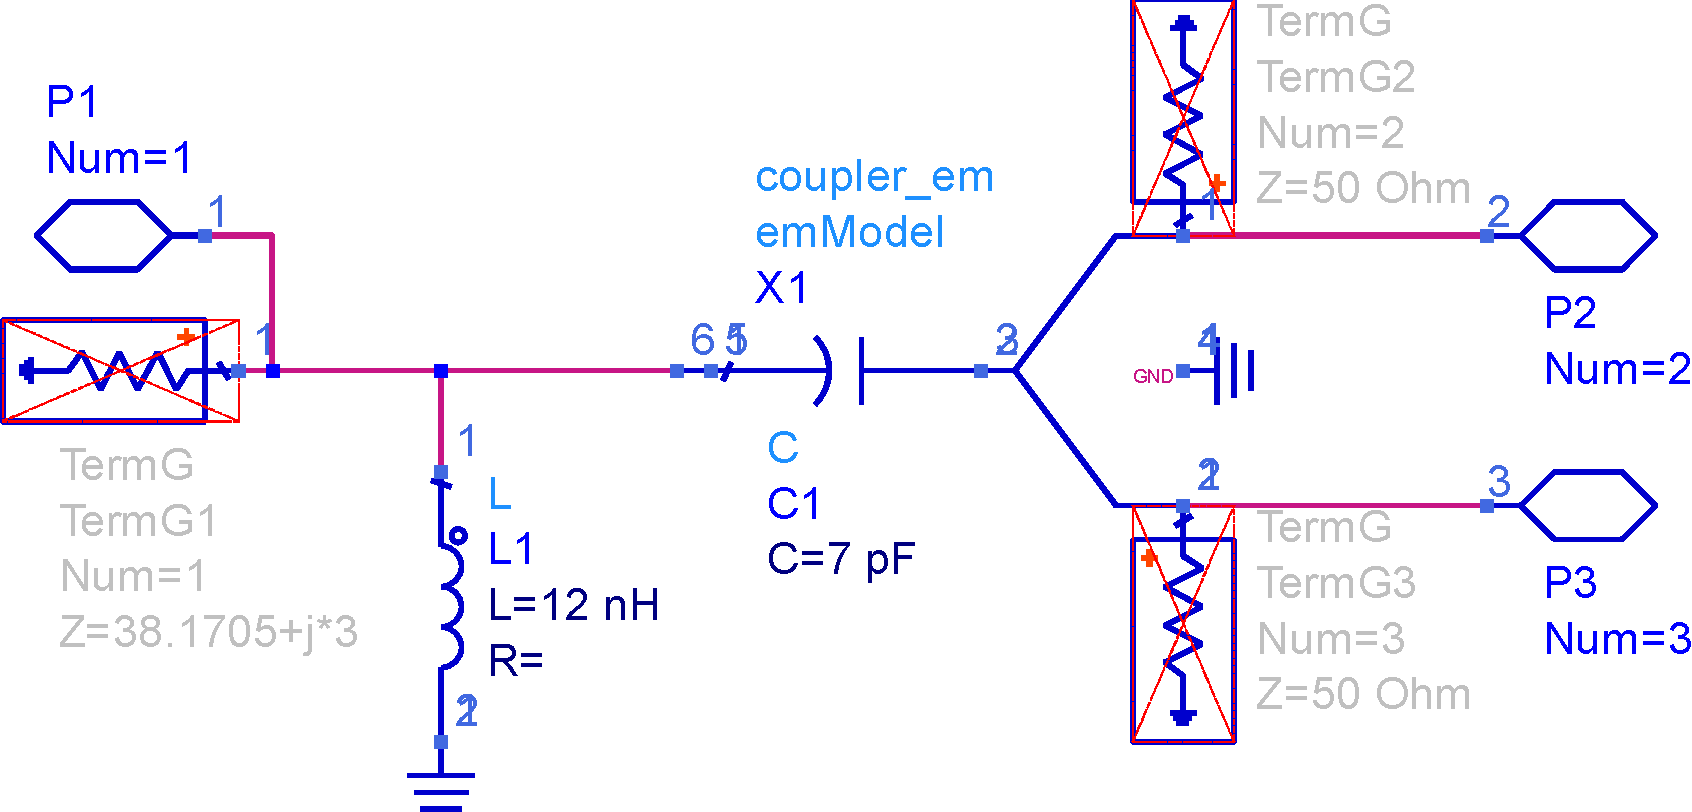
\includegraphics[width=\textwidth]{coupler-match.pdf}
		\caption{}%
		\label{fig:coupler-match}
	\end{subfigure}
	\caption{%
		(а) Топология и 
		(б) схема согласования делителя
	}%
	\label{fig:coupler-em-sch}
\end{figure}

На Рисунке \ref{fig:IPL-coupler-results} показаны результаты моделирования входного тракта с учетом делителя мощности.

\begin{figure}[H]
	\centering
	\begin{subfigure}[c]{0.49\textwidth}
		\centering
		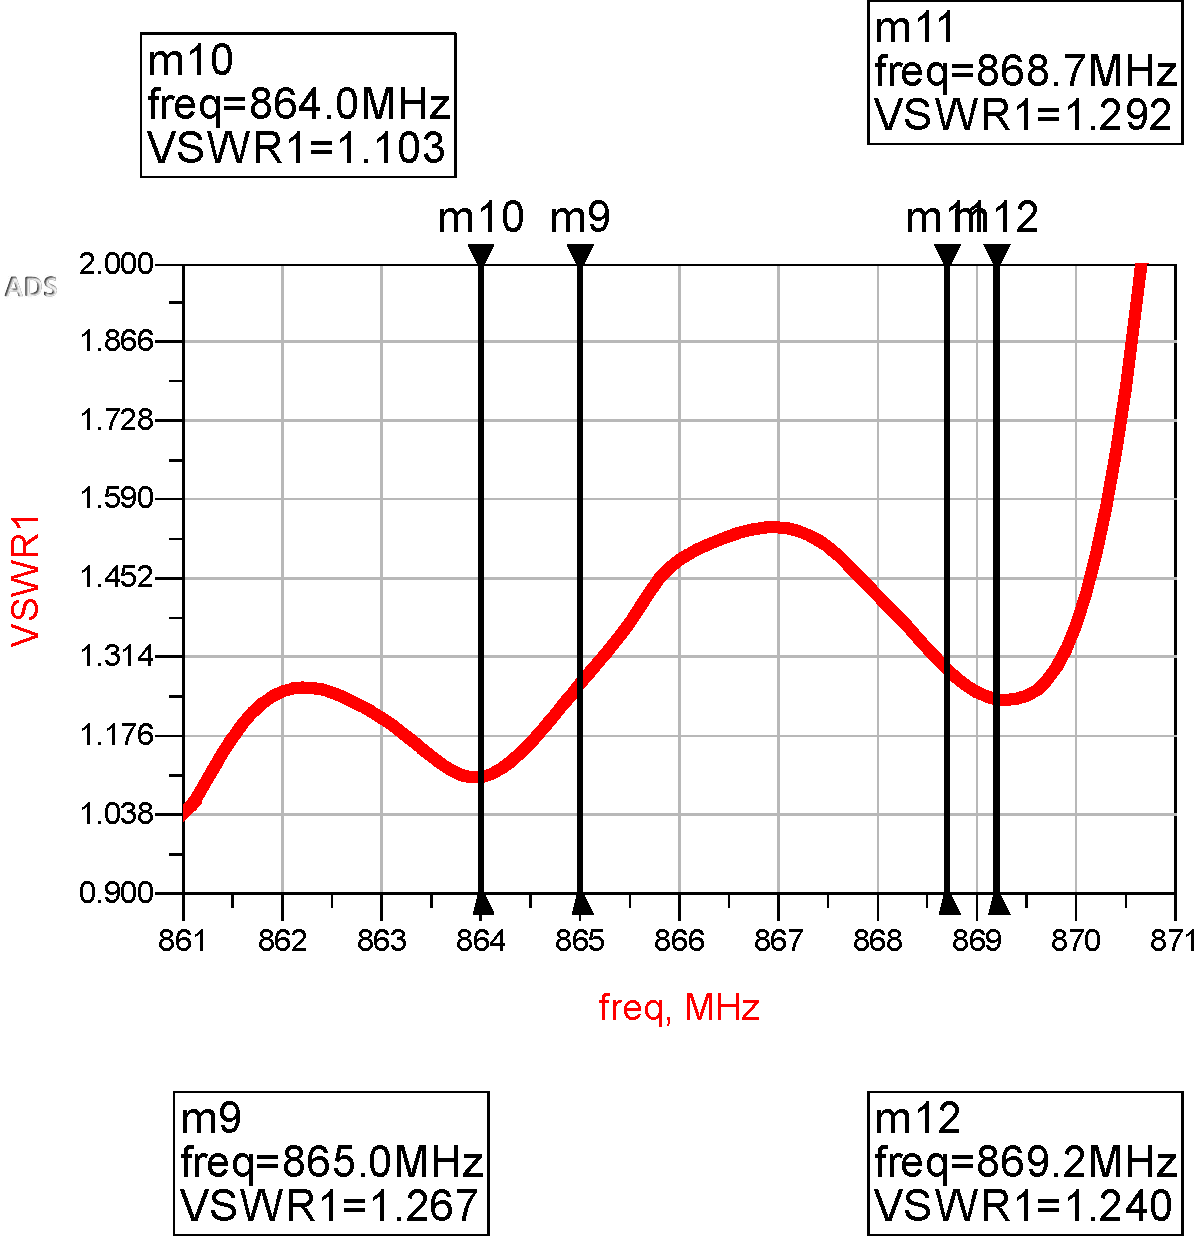
\includegraphics[width=\textwidth]{IPL-coupler-VSWR.pdf}
		\caption{}%
		\label{fig:IPL-coupler-VSWR}
	\end{subfigure}
	\hfill
	\begin{subfigure}[c]{0.49\textwidth}
		\centering
		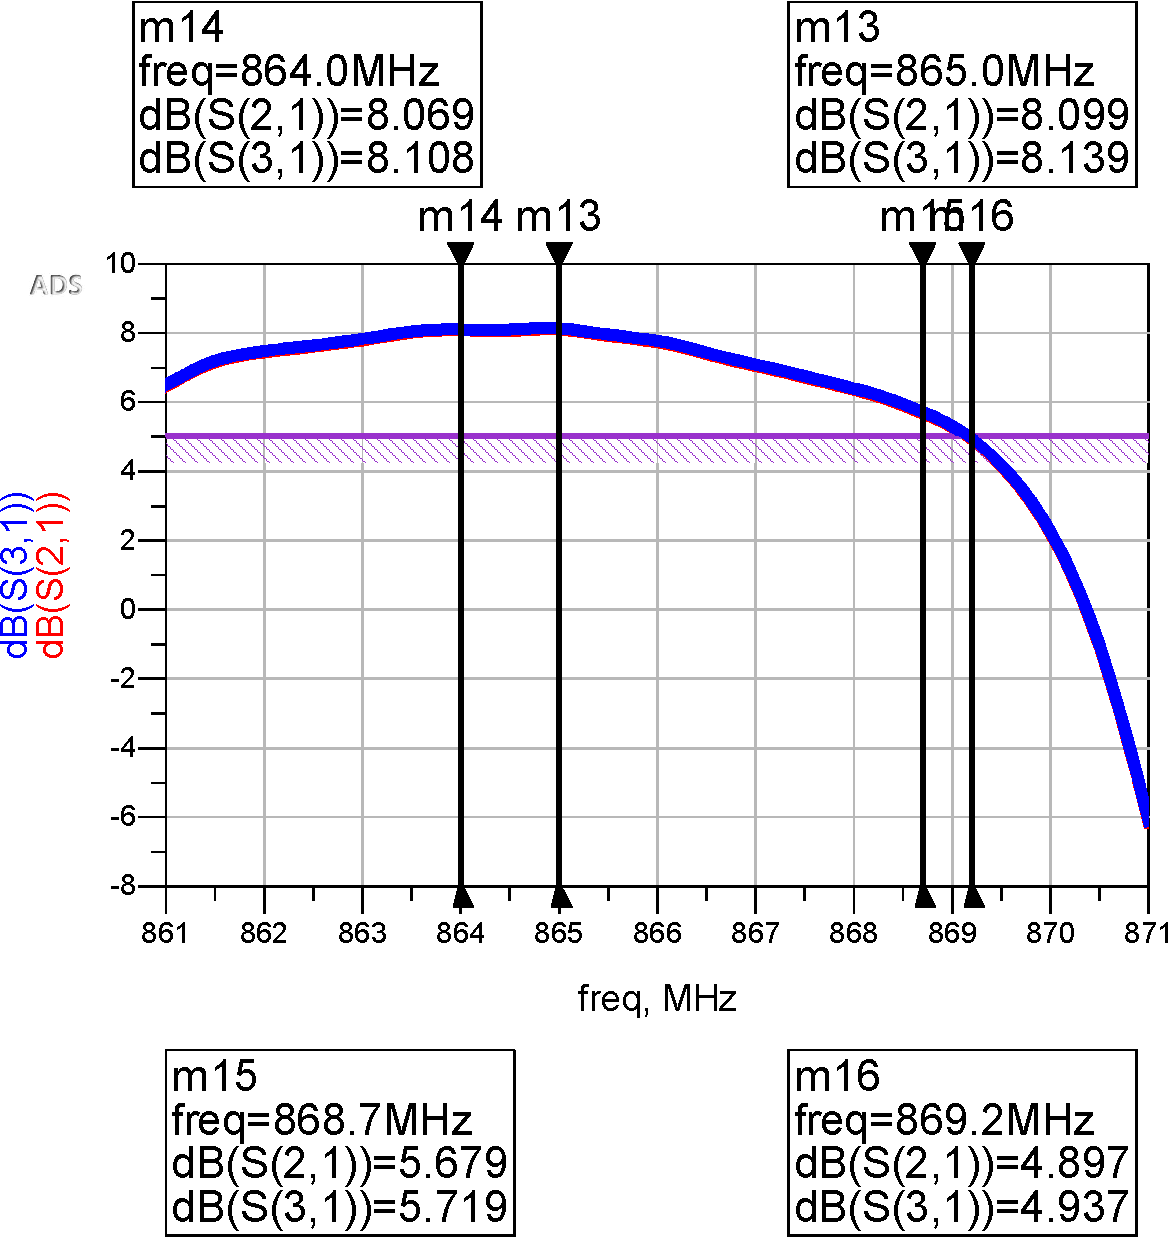
\includegraphics[width=\textwidth]{IPL-coupler-trans.pdf}
		\caption{}%
		\label{fig:IPL-coupler-trans}
	\end{subfigure}
	\caption{%
		(а) Топология и 
		(б) схема согласования делителя
	}%
	\label{fig:IPL-coupler-results}
\end{figure}

\subsection{Составление библиотек ЭКБ.}

Дальнейшая работа будет проводиться в Altium Designer. На основе документации производителей и требований ГОСТ 2.710-81 и ГОСТ 2.743-91 составлены библиотеки УГО и посадочных мест используемых компонентов.

Составленные библиотеки находятся в репозитории проекта в соответствующем разделе.

\subsection{Разработка электрической схемы.}

Основываясь на результатах проведенного моделирования и ориентируясь на рекомендации производителей в соответствии с ГОСТ 2.702-2011 была разработана электрическая принципиальная схема устройства. Схема разбита на несколько листов.

\begin{figure}[H]
	\centering
	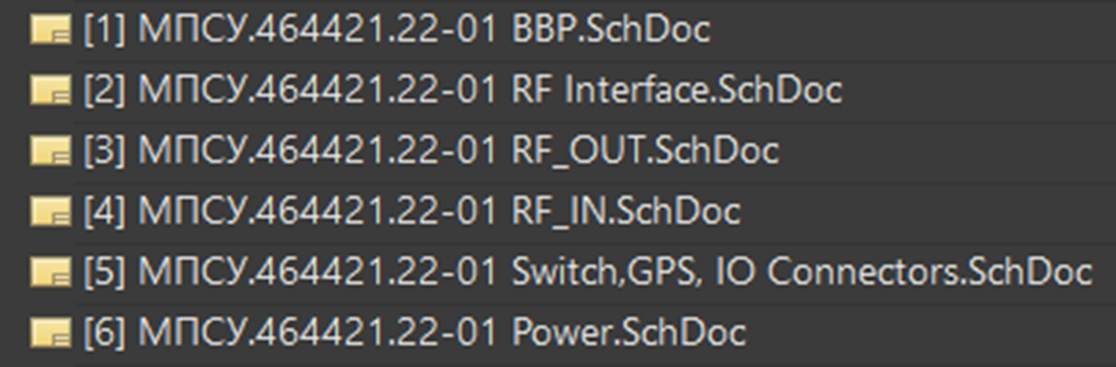
\includegraphics[width=0.6\textwidth,keepaspectratio]{bs-sch-grouping.png}
	\caption{Разбиение схемы электрической принципиальной}%
	\label{fig:bs-sch-grouping}
\end{figure}

Эскиз листа со схемой приёмного канала показан на Рисунке \ref{fig:bs-sch-rf-in}

\begin{figure}[H]
	\centering
	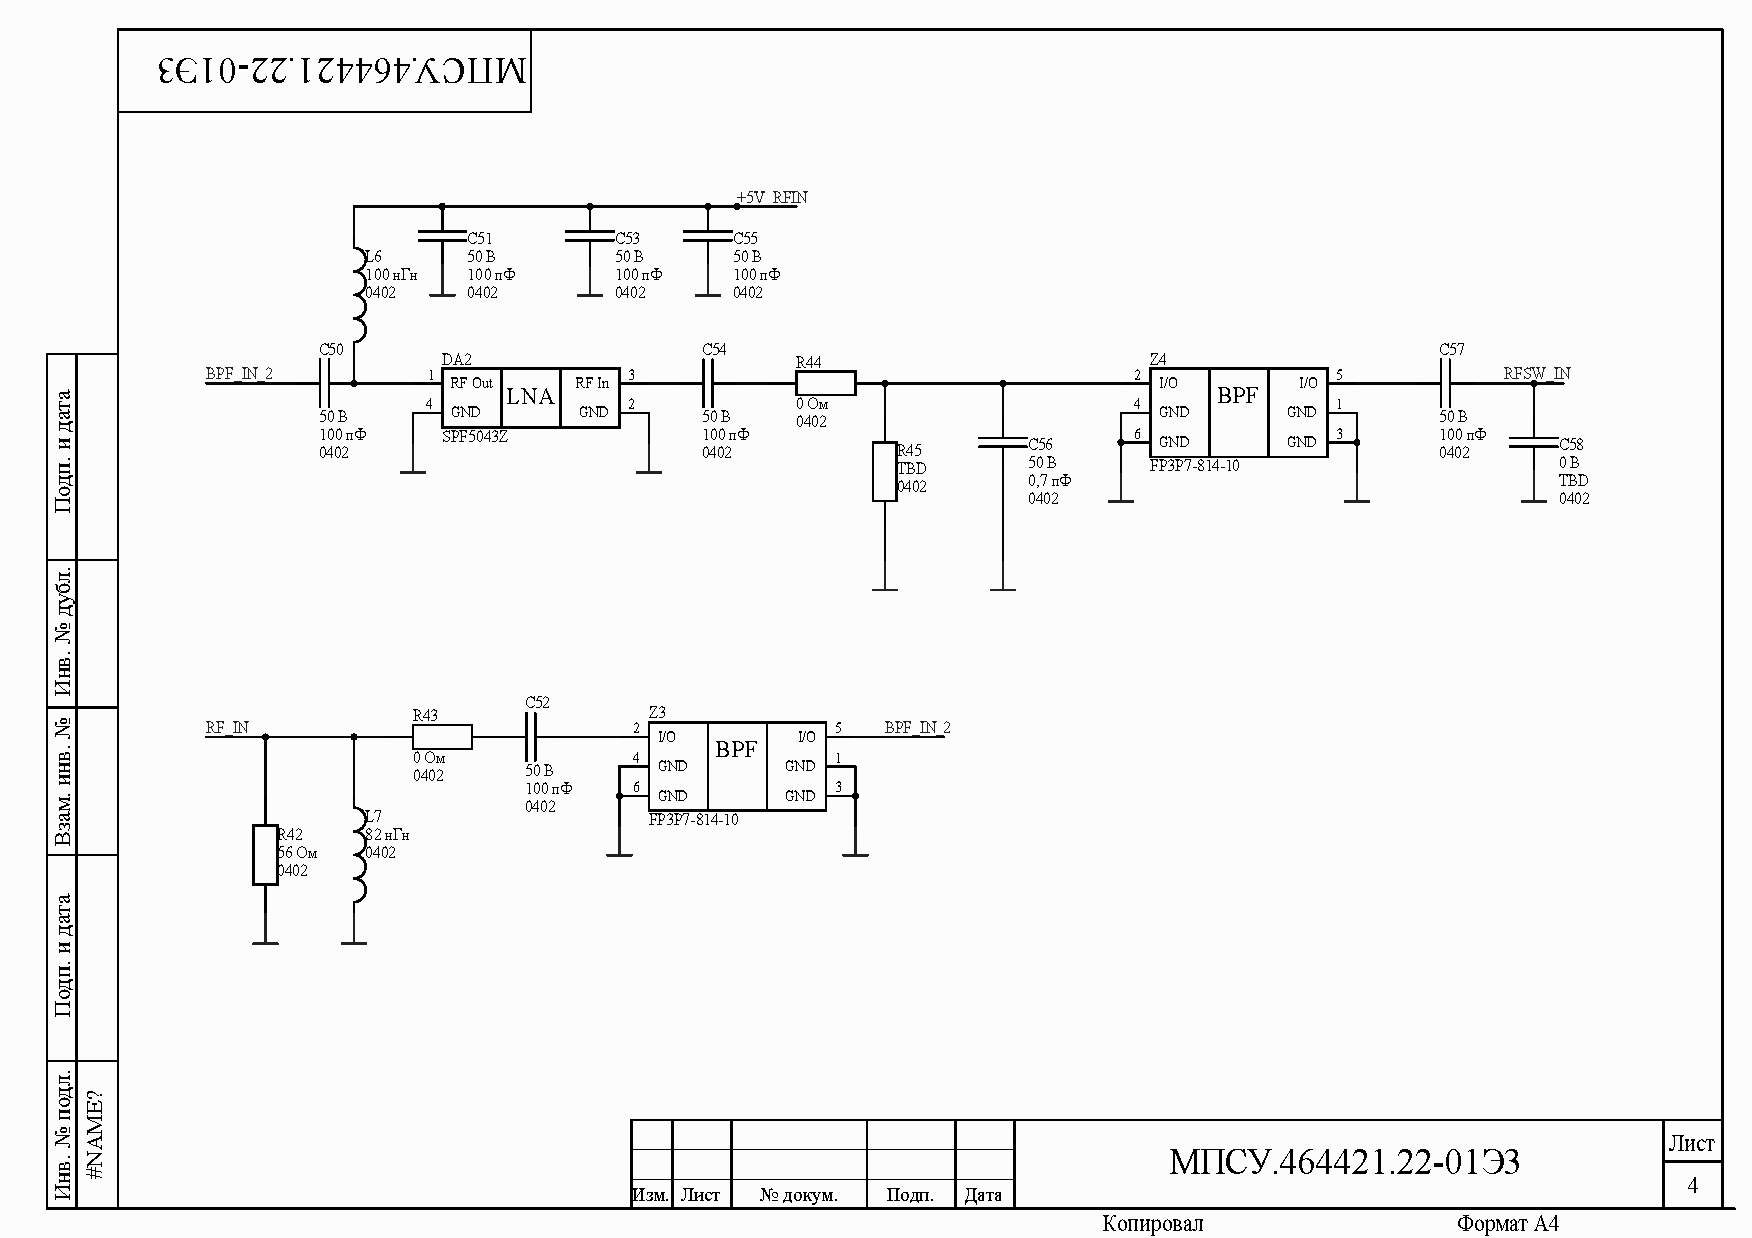
\includegraphics[width=\textwidth,keepaspectratio]{bs-sch-rf-in.pdf}
	\caption{Эскиз одного из листов Э3 на БС.}%
	\label{fig:bs-sch-rf-in}
\end{figure}

Более подробно про экспорт документации будет рассказано в главе \ref{sect:project-docs}.

\subsection{Проектирование топологии.} \label{sect:bs-topology}

На основании схемы электрической принципиальной, с использованием составленных ранее библиотек и с учетом возможностей современных производителей печатных плат была спроектирована топология печатной платы устройства. На Рисунке \ref{fig:bs-stackup} показано отображение стека платы в Altium Designer.

\begin{figure}[H]
	\centering
	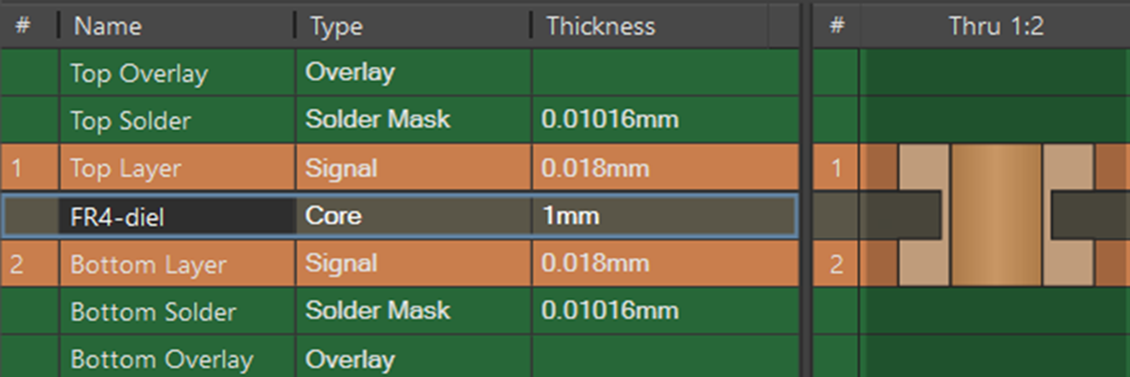
\includegraphics[width=0.7\textwidth,keepaspectratio]{bs-stackup.png}
	\caption{Стек печатной платы БС}%
	\label{fig:bs-stackup}
\end{figure}

На следующих рисунках показано отображение основной информации о печатной плате и печатном узле БС.

\begin{figure}[H]
	\centering
	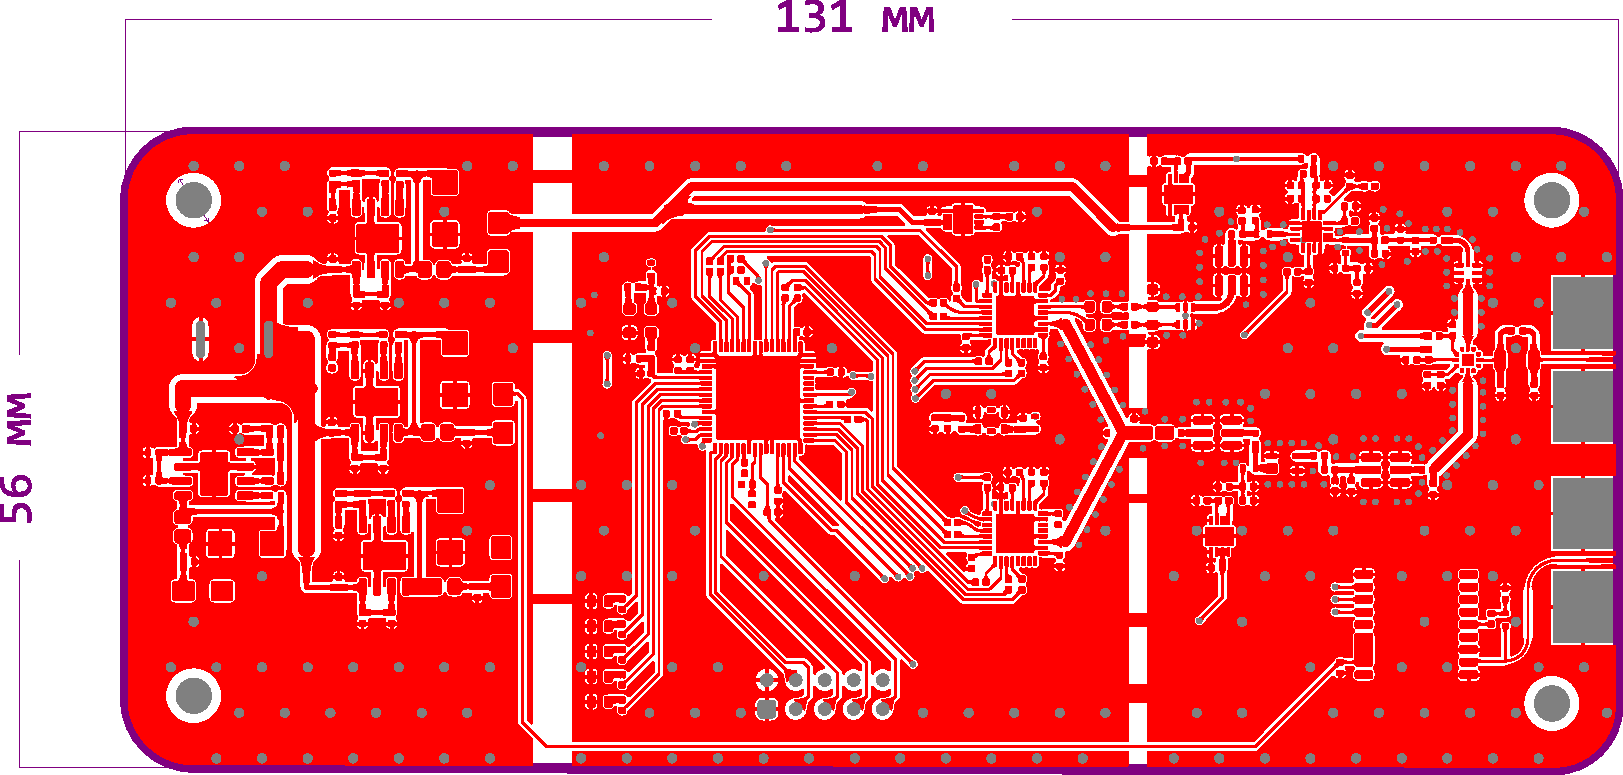
\includegraphics[width=\textwidth,keepaspectratio]{BS-Top Layer.pdf}
	\caption{Топология верхнего слоя}%
\end{figure}

\begin{figure}[H]
\centering
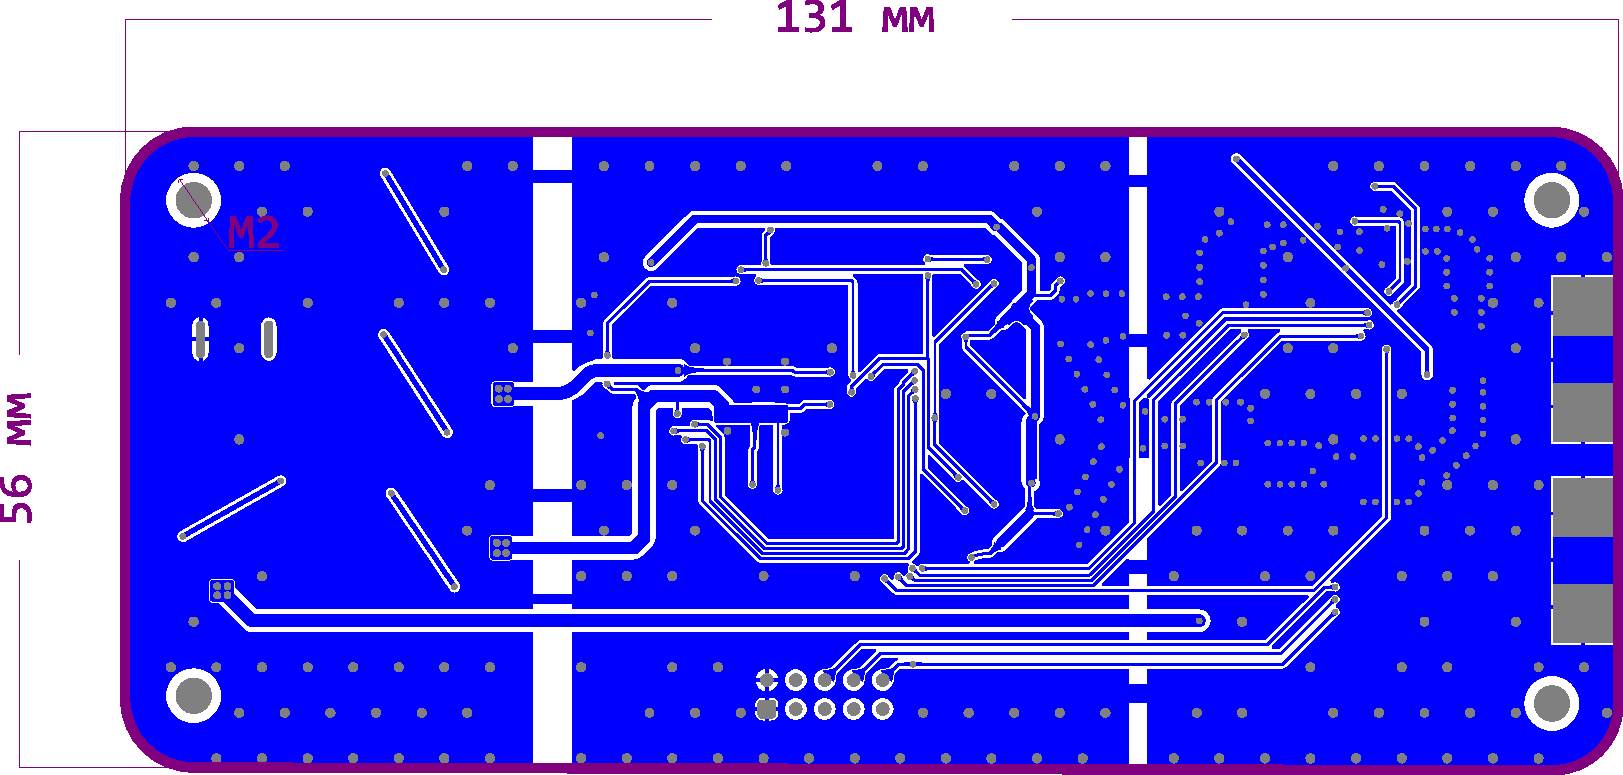
\includegraphics[width=\textwidth,keepaspectratio]{BS-Bottom Layer.pdf}
\caption{Топология нижнего слоя}%
\end{figure}


\begin{figure}[H]
	\centering
	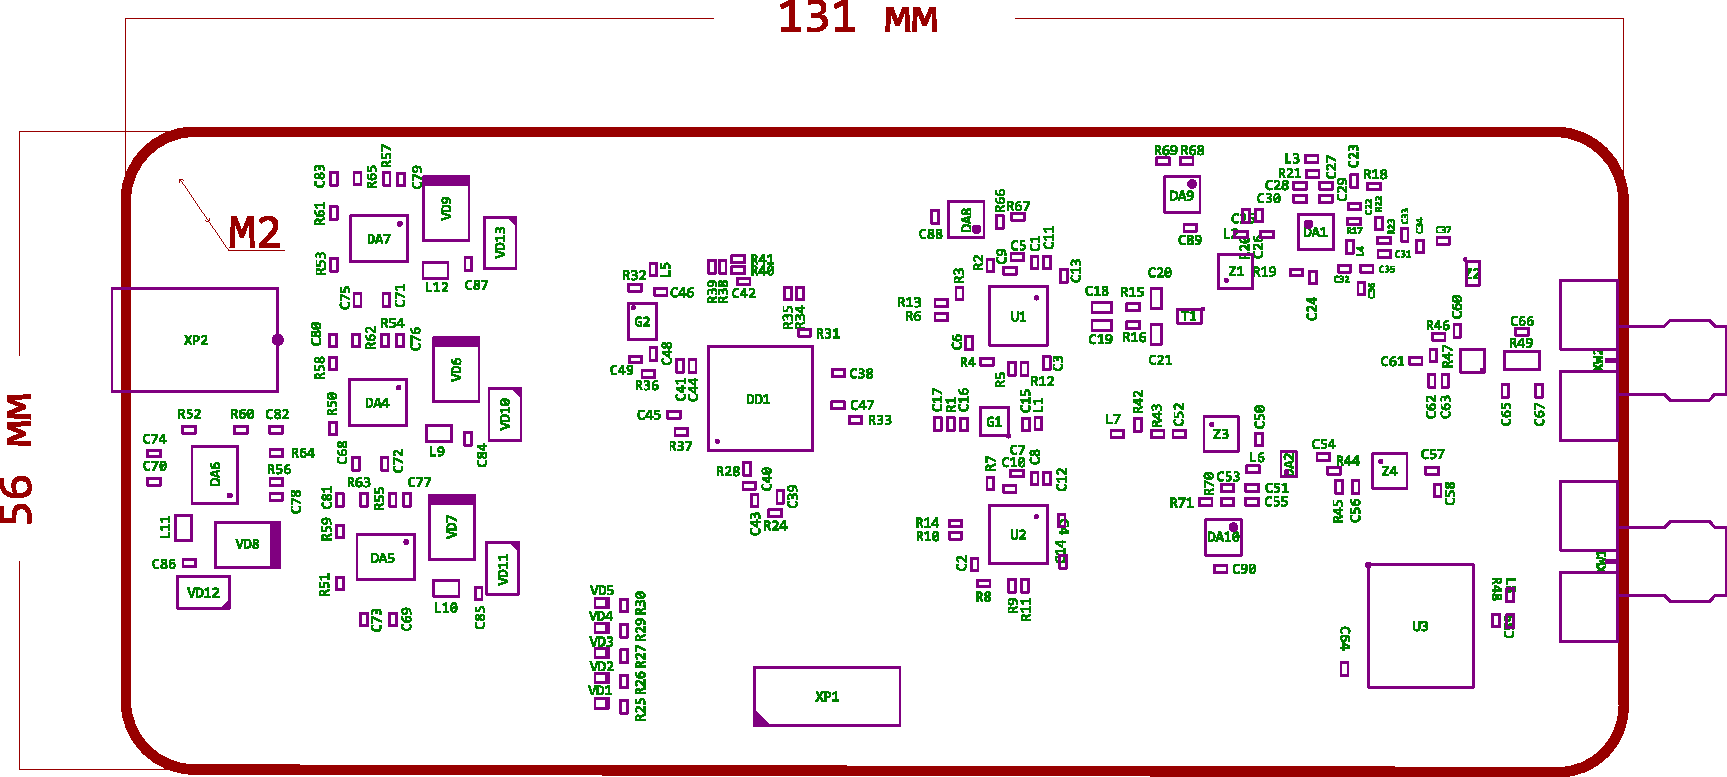
\includegraphics[width=\textwidth,keepaspectratio]{BS-Assembly Drawing.pdf}
	\caption{Эскиз сборочного чертёжа}%
\end{figure}

\subsection{Трёхмерная модель и поддерживающая рамка.}

Altium Designer позволяет отображать фотореалистичные модели разработанных печатных плат. С учетом этого, ещё на стадии формирования библиотек были созданы 3D модели компонентов. Итоговый вид платы можно увидеть на Рисунке \ref{fig:3D-Board}.

\begin{figure}[H]
	\centering
	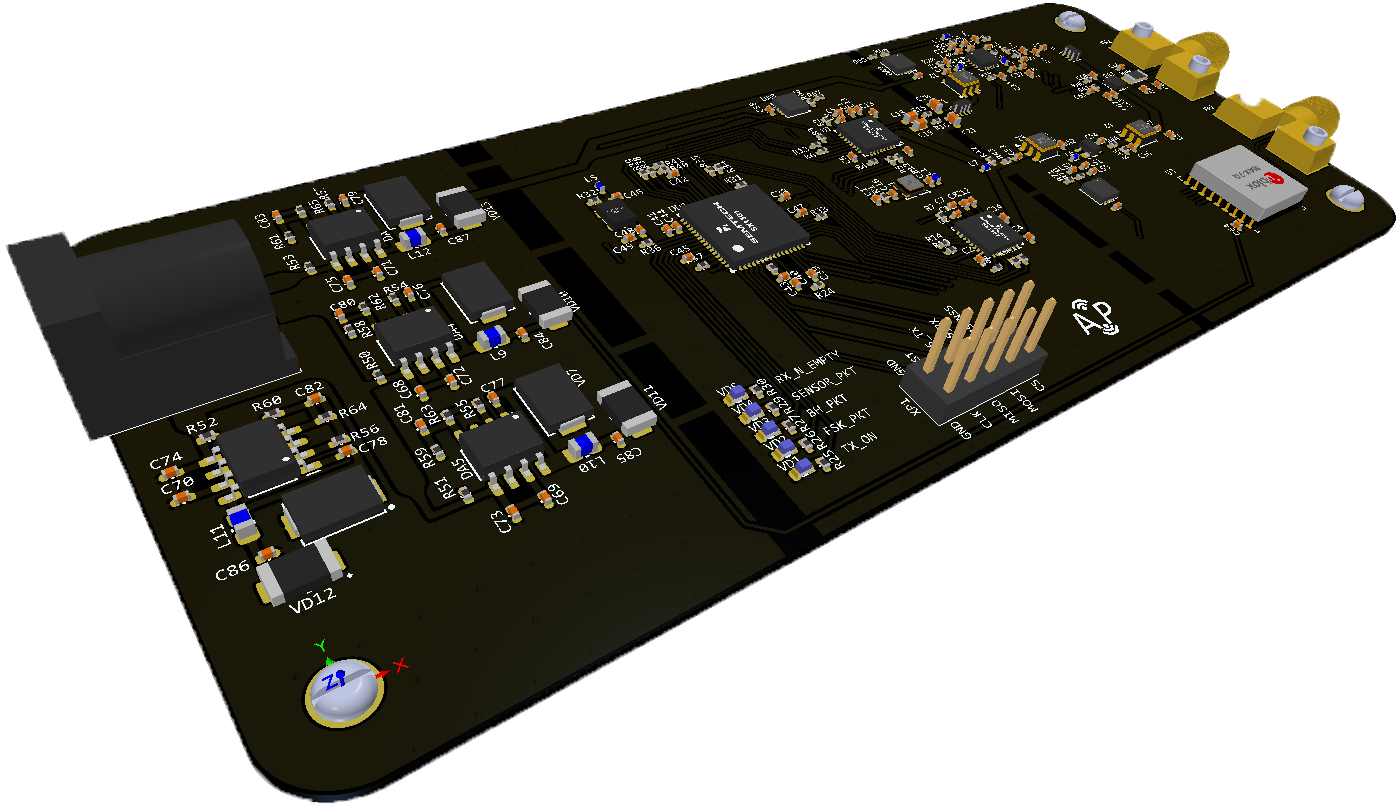
\includegraphics[width=\textwidth,keepaspectratio]{3D-Board.png}
	\caption{трехмерная модель платы, изометрический вид.}%
	\label{fig:3D-Board}
\end{figure}

Также для удобства эксплуатации модуля была разработана поддерживающая рамка, показанная на Рисунке \ref{fig:BS-Frame}. Итоговая сборка показана на Рисунке \ref{fig:bs-3d-framed}.

\begin{figure}[H]
	\centering
	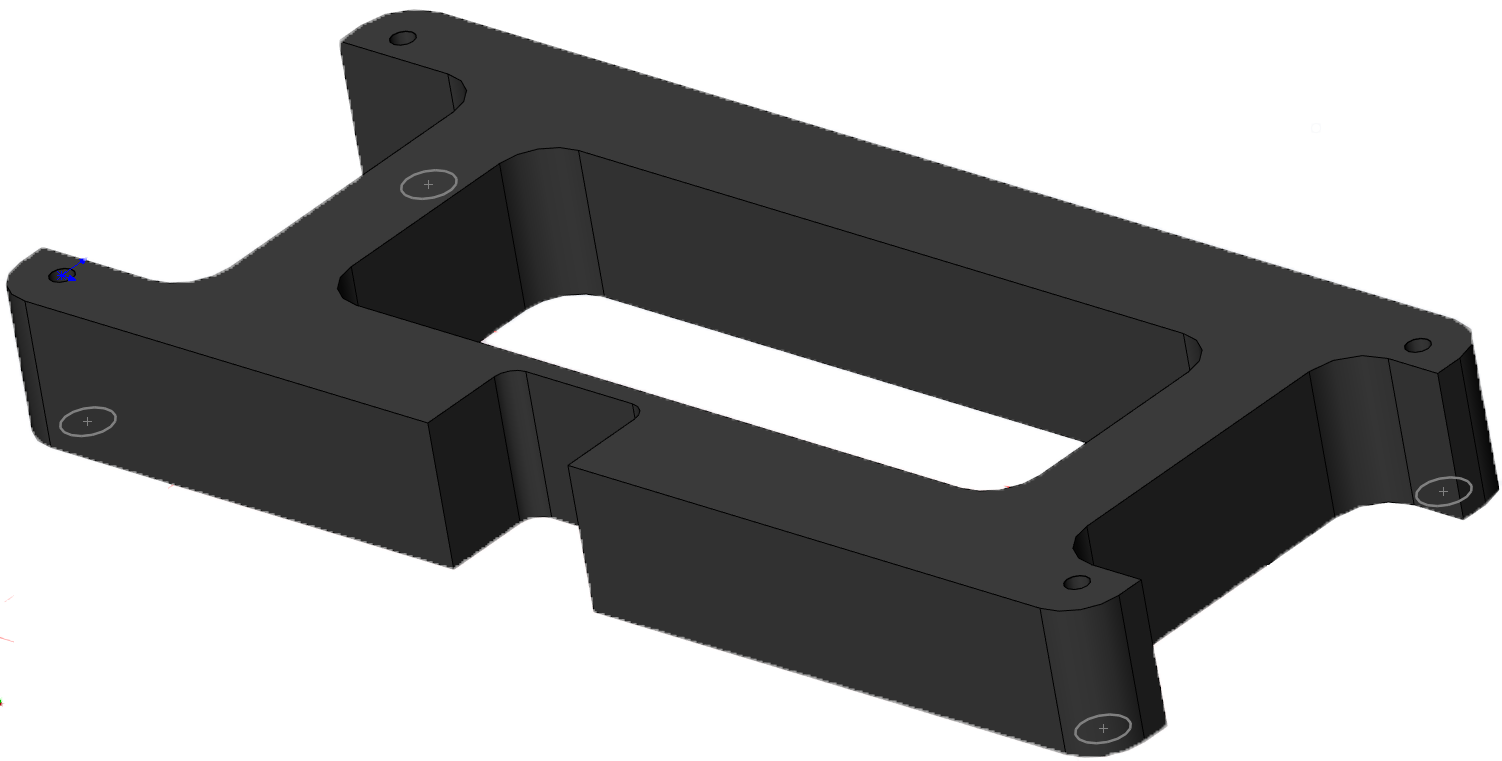
\includegraphics[width=\textwidth,keepaspectratio]{BS-Frame.png}
	\caption{трёхмерная модель рамки, изометрический вид сверху.}%
	\label{fig:BS-Frame}
\end{figure}

\begin{figure}[H]
	\centering
	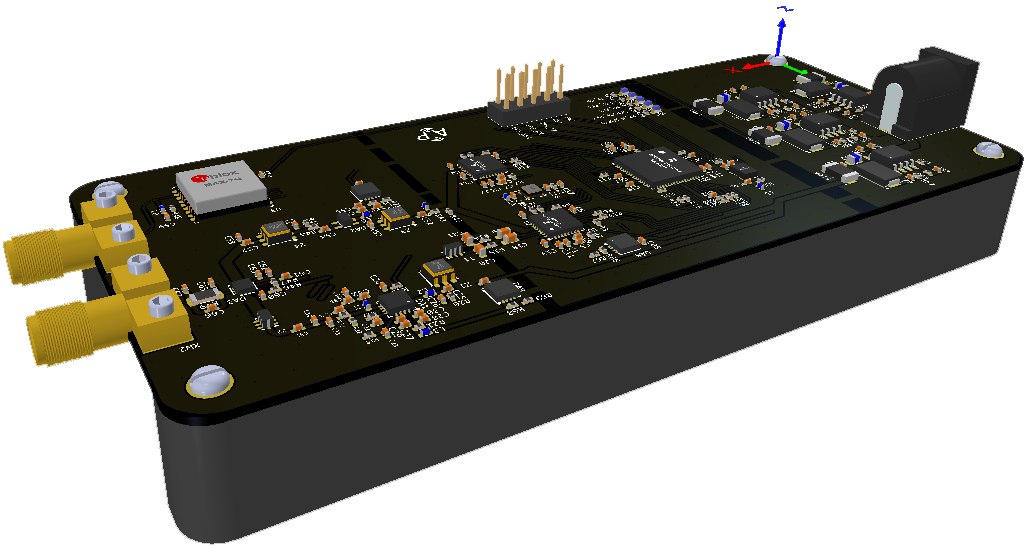
\includegraphics[width=\textwidth,keepaspectratio]{bs-3d-framed.png}
	\caption{трехмерная модель сборки. Изометрический вид сверху.}%
	\label{fig:bs-3d-framed}
\end{figure}


\subsection{Разработка платы измерения параметров усилителя.} \label{sect:bs-oa-mes}

Как упоминалось в Главе \ref{sect:bs-topology}, для получения более точных характеристик усилителя, была разработана плата измерения. Электрическая схема включения усилителя аналогична схеме включения в основном проекте – по входу и выходу установлены универсальные схемы согласования - набор из двух последовательных и двух параллельных компонентов. Этого набора достаточно для согласования большинства устройств.

\begin{figure}[H]
	\centering
	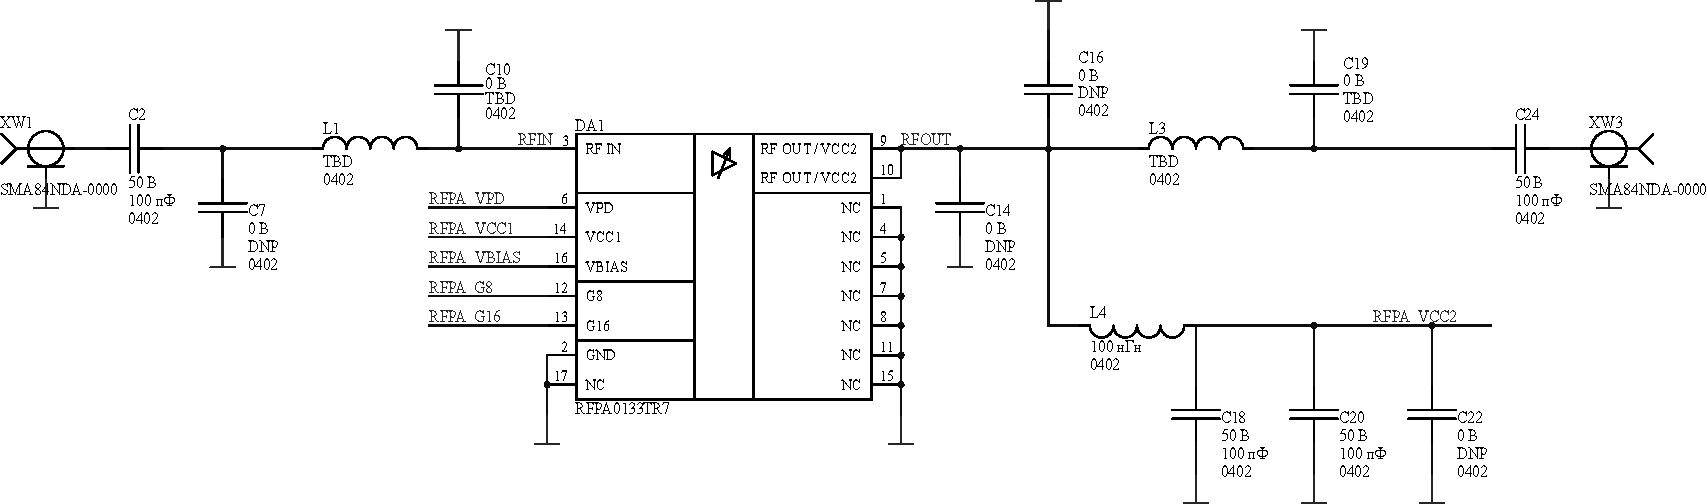
\includegraphics[width=\textwidth,keepaspectratio]{pa-measuring-sch.pdf}
	\caption{электрическая схема включения УМ}%
	\label{fig:pa-measuring-sch}
\end{figure}

 Дополнительно была создана линия для калибровки средств измерения. Она является полной копией основной линии за исключением измеряемого компонента.

\begin{figure}[H]
	\centering
	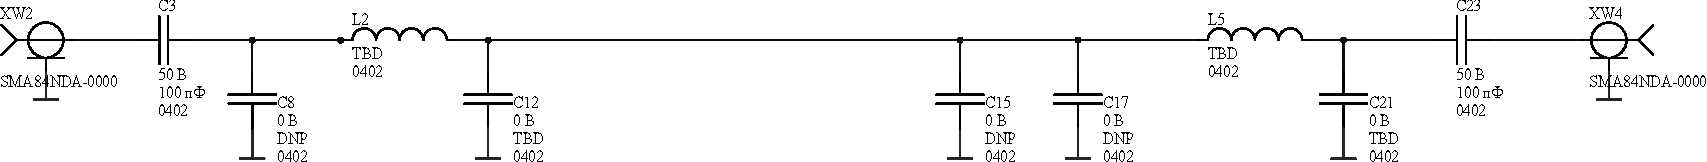
\includegraphics[width=\textwidth,keepaspectratio]{pa-measuring-cal-line-sch.pdf}
	\caption{линия для калибровки}%
	\label{fig:pa-measuring-cal-line-sch}
\end{figure}

Для уменьшения количества неоднородностей ширину линии была выбрана равной ширине контактных площадок микросхемы усилителя. 

Чтобы обеспечить достоверность измерения не только амплитуды, но и фазы, нужно удостовериться в полной идентичности цепи калибровки и цепей включения компонента. Для удовлетворения данного требования выходные и выходные цепи линии измерения были скопированы и перенесены на топологическом уровне. 

Внешний вид разработанной платы показан на Рисунке \ref{fig:pa-measuring-topview}. Сверху находится измерительная линия, снизу – линия калибровки.

\begin{figure}[H]
	\centering
	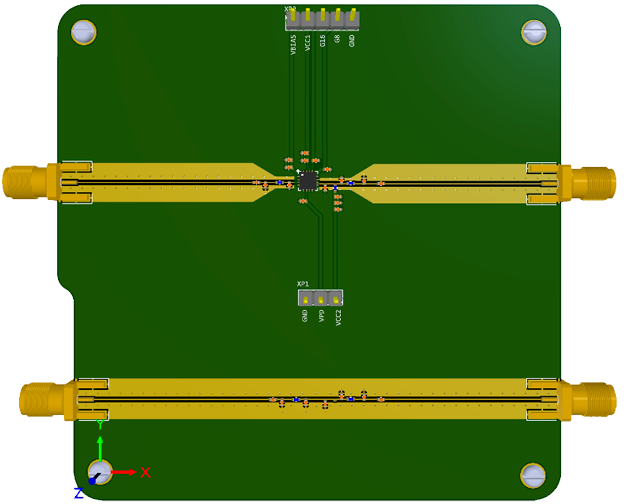
\includegraphics[width=\textwidth,keepaspectratio]{pa-measuring-topview.png}
	\caption{3D модель измерительной платы. Вид сверху.}%
	\label{fig:pa-measuring-topview}
\end{figure}




	\section{Разработка мобильного модуля.}
\subsection{Разработка структурной схемы.}

Существует несколько вариантов построения оконечного модуля:
\begin{enumerate}
	\item На основе микроконтроллера общего назначения и специализированного приемопередатчика  Semtech из серии SX12**.
	\item На основе готовых микросборок.
	\item На основе специализированных микроконтроллеров.
\end{enumerate}

\justifying В данной работе применяется второй вариант ввиду его простоты. В качестве центрального устройства будет использоваться чип AcSiP S76S. Данный чип представляет из себя микросборку из энергоэффективного МК \linebreak STM32L073xZ, приемопередатчика SX1276 и необходимой периферии. Упрощенная структурная схема МСБ, предоставляемая производителем показана на Рисунке~\ref{fig:S76S-struct}.

\begin{figure}[H]
	\centering
	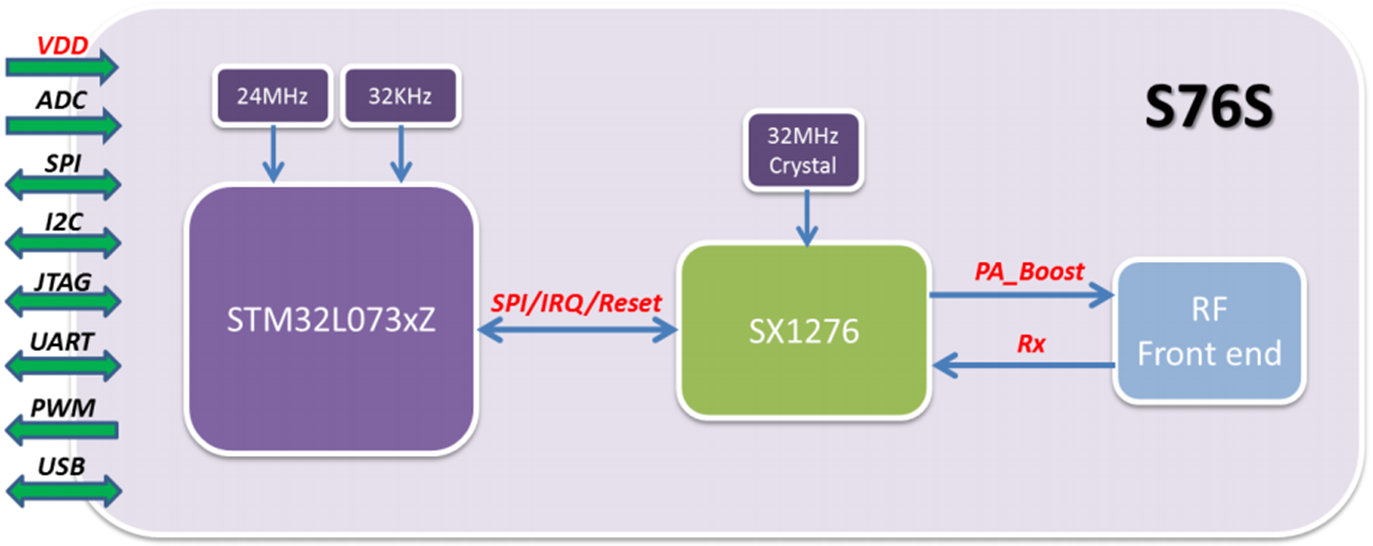
\includegraphics[width=\textwidth,keepaspectratio]{S76S-struct.png}
	\caption{базовая структурная схема AcSiP S76S.}%
	\label{fig:S76S-struct}
\end{figure}

Структурная схема разрабатываемого мобильного модуля показана на Рисунке~\ref{fig:MM-StructSch}

\begin{figure}[H]
	\centering
	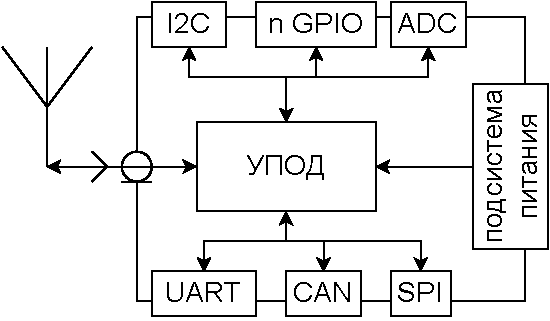
\includegraphics[width=0.8\textwidth,keepaspectratio]{MM-StructSch.pdf}
	\caption{Структурная схема разрабатываемого устройства.\\ УПОД – устройство приёмопередачи и обработки данных.}%
	\label{fig:MM-StructSch}
\end{figure}

\subsection{Разработка подсистемы питания.}

Единственным потребителем электрической энергии на плате является чип S76S, для обеспечения его работы требуется напряжение от 2,4 до 3,6 В. Для обеспечения работы от аккумуляторной батареи с возможностью её зарядки требуется контроллер заряда батареи и стабилизатор напряжения. 

\begin{figure}[H]
	\centering
	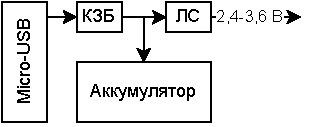
\includegraphics[width=0.7\textwidth,keepaspectratio]{MM-PowerSch.pdf}
	\caption{Структурная схема подсистемы питания МОУ}
	\label{fig:MM-PowerSch}
\end{figure}

\begin{itemize}
	\item На роль линейного стабилизатора выберем описанный ранее LT1965EDD.
	\item Контроллером заряда батареи будет MCP73831T-2ACI/OT с выходным напряжением из ряда 4,2, 4,35, 4,40, 4,50 В и регулируемым выходным током от 15 до 500 мА
	\begin{figure}[H]
		\centering
		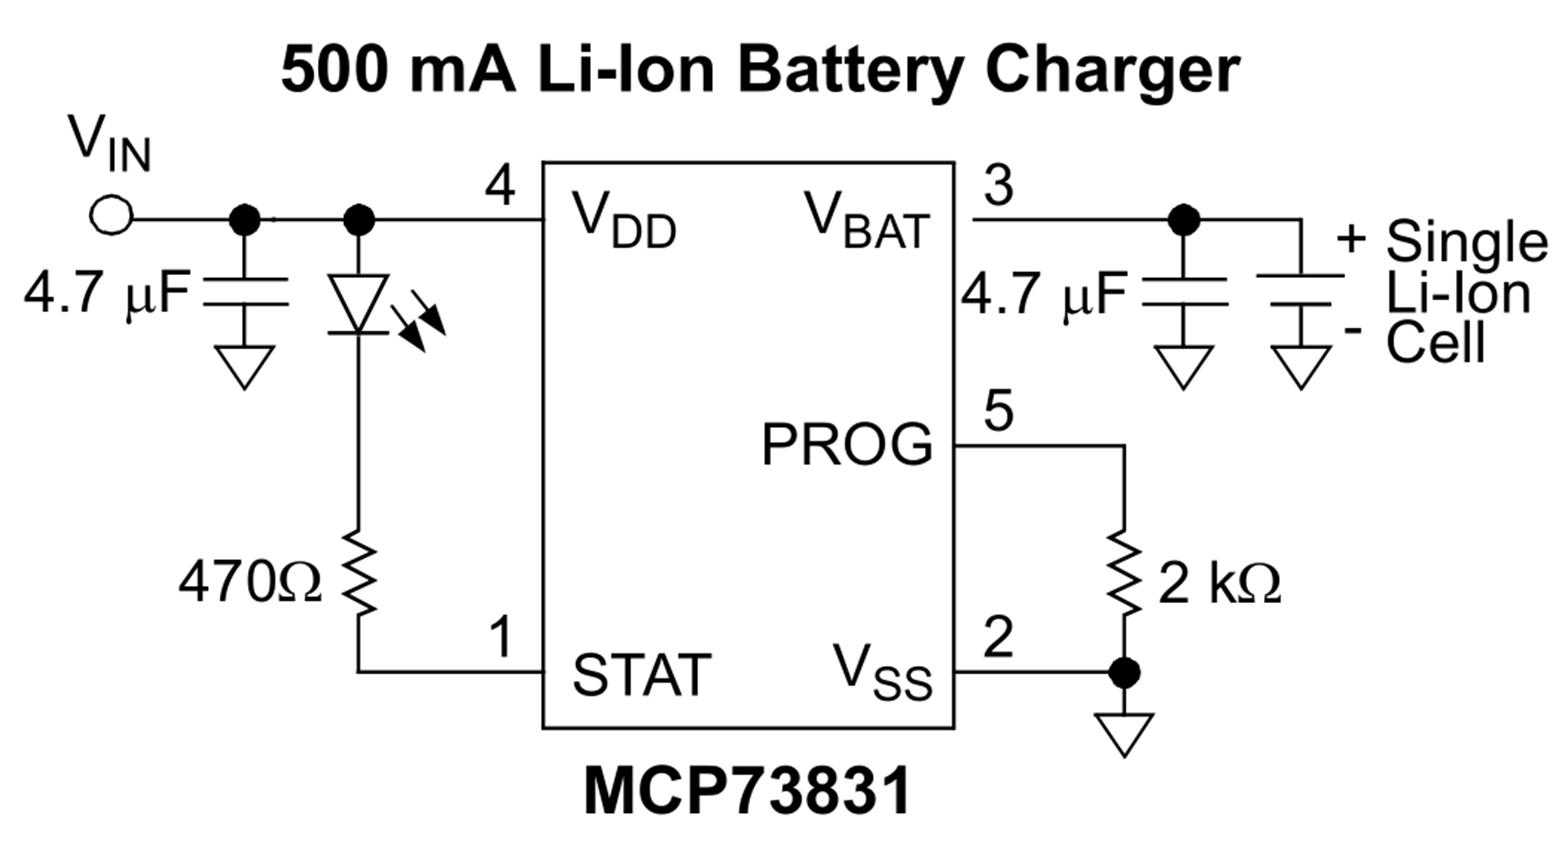
\includegraphics[width=0.8\textwidth,keepaspectratio]{charge-controller.png}
		\caption{стандартная схема включения КЗБУ}
		\label{fig:charge-controller}
	\end{figure}
\end{itemize}

Выбранные компоненты были добавлены в составленную ранее библиотеку.

\subsection{Составление электрической схемы.}

Основываясь на предполагаемых сценариях применения итогового устройства и ориентируясь на рекомендации производителей была составлена электрическая принципиальная схема устройства. Полная документация на устройство будет находиться в репозитории проекта в соответствующем разделе. Более подробно про экспорт документации будет рассказано в главе \ref{sect:project-docs}.

\subsection{Проектирование топологии.}

На основании схемы электрической принципиальной, с использованием составленных ранее библиотек и с учетом возможностей современных производителей печатных плат были спроектированы два варианта топологии печатной платы устройства. Они показаны на рисунках \ref{fig:mb-topology} и \ref{fig:ms-topology}. Первый вариант более удобен для разработки, а также предполагает возможность установки аккумулятора большего объёма. Второй вариант более компактный и предоставляет пользователю выбор типа аккумулятора - со штырьковым разъёмом либо формата АА.

\begin{figure}[H]
	\centering
	\begin{subfigure}[c]{0.49\textwidth}
		\centering
		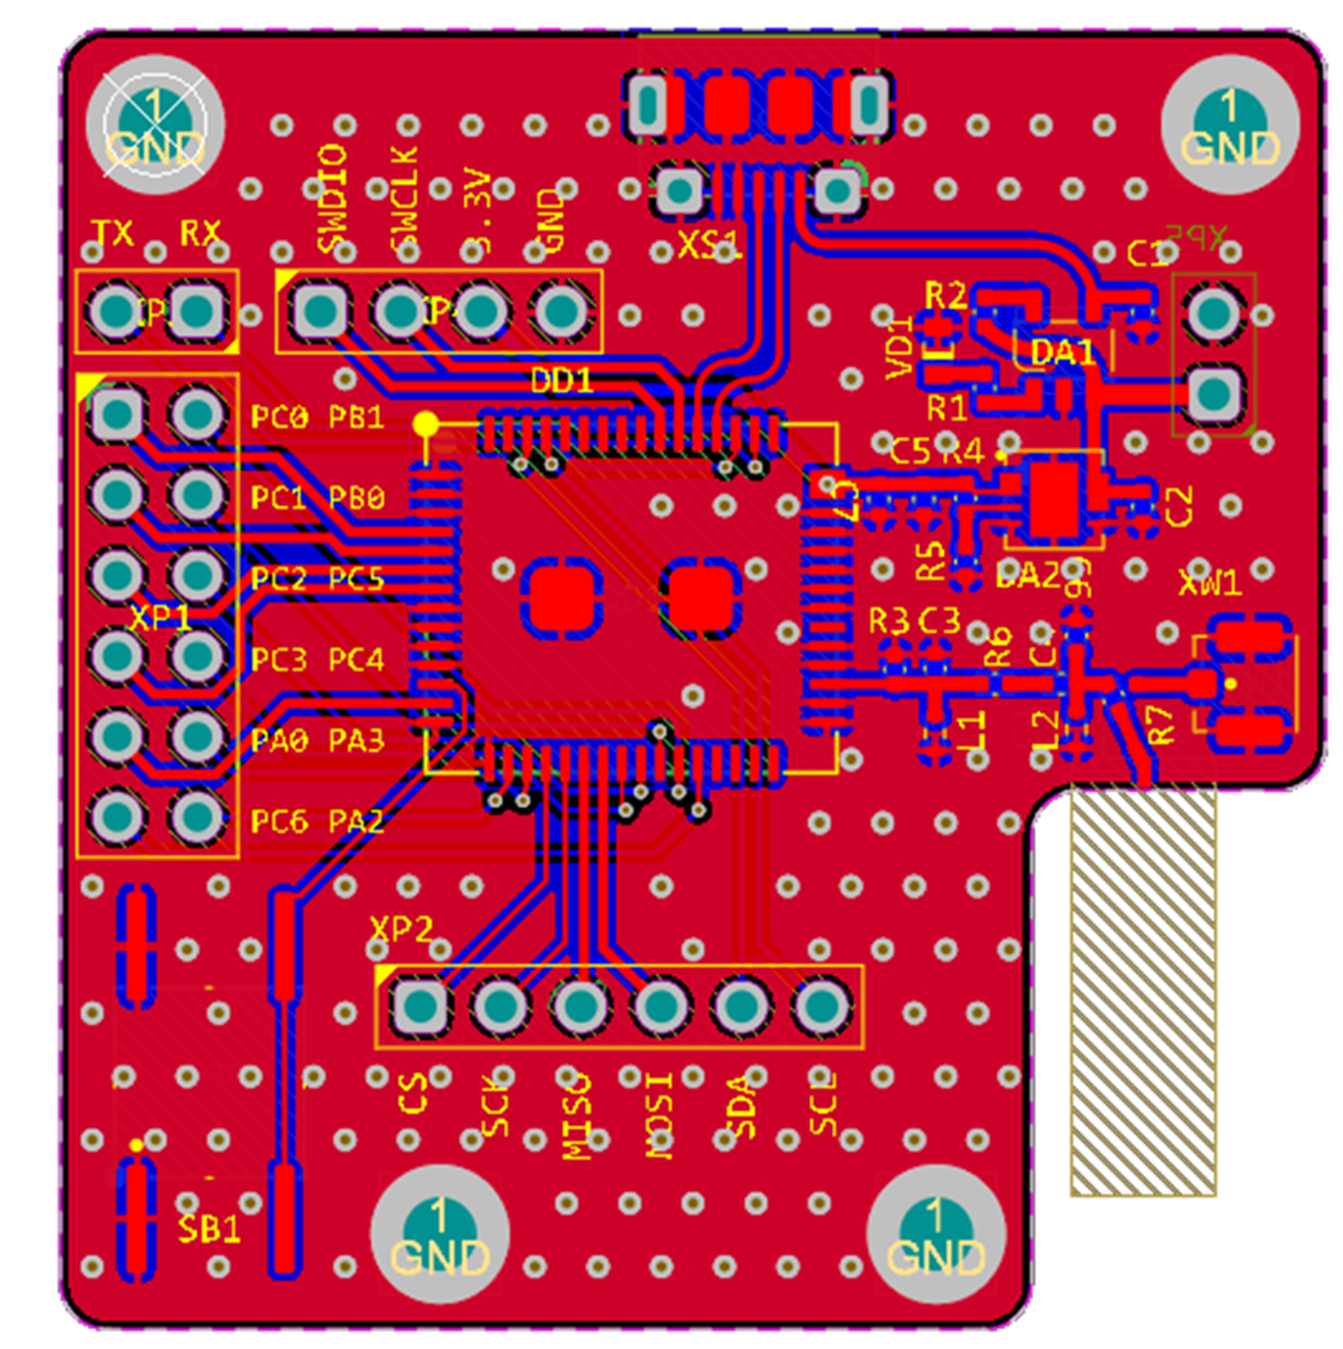
\includegraphics[height=15em]{mb-topology.png}
		\caption{}%
		\label{fig:mb-topology}
	\end{subfigure}
	\hfill
	\begin{subfigure}[c]{0.49\textwidth}
		\centering
		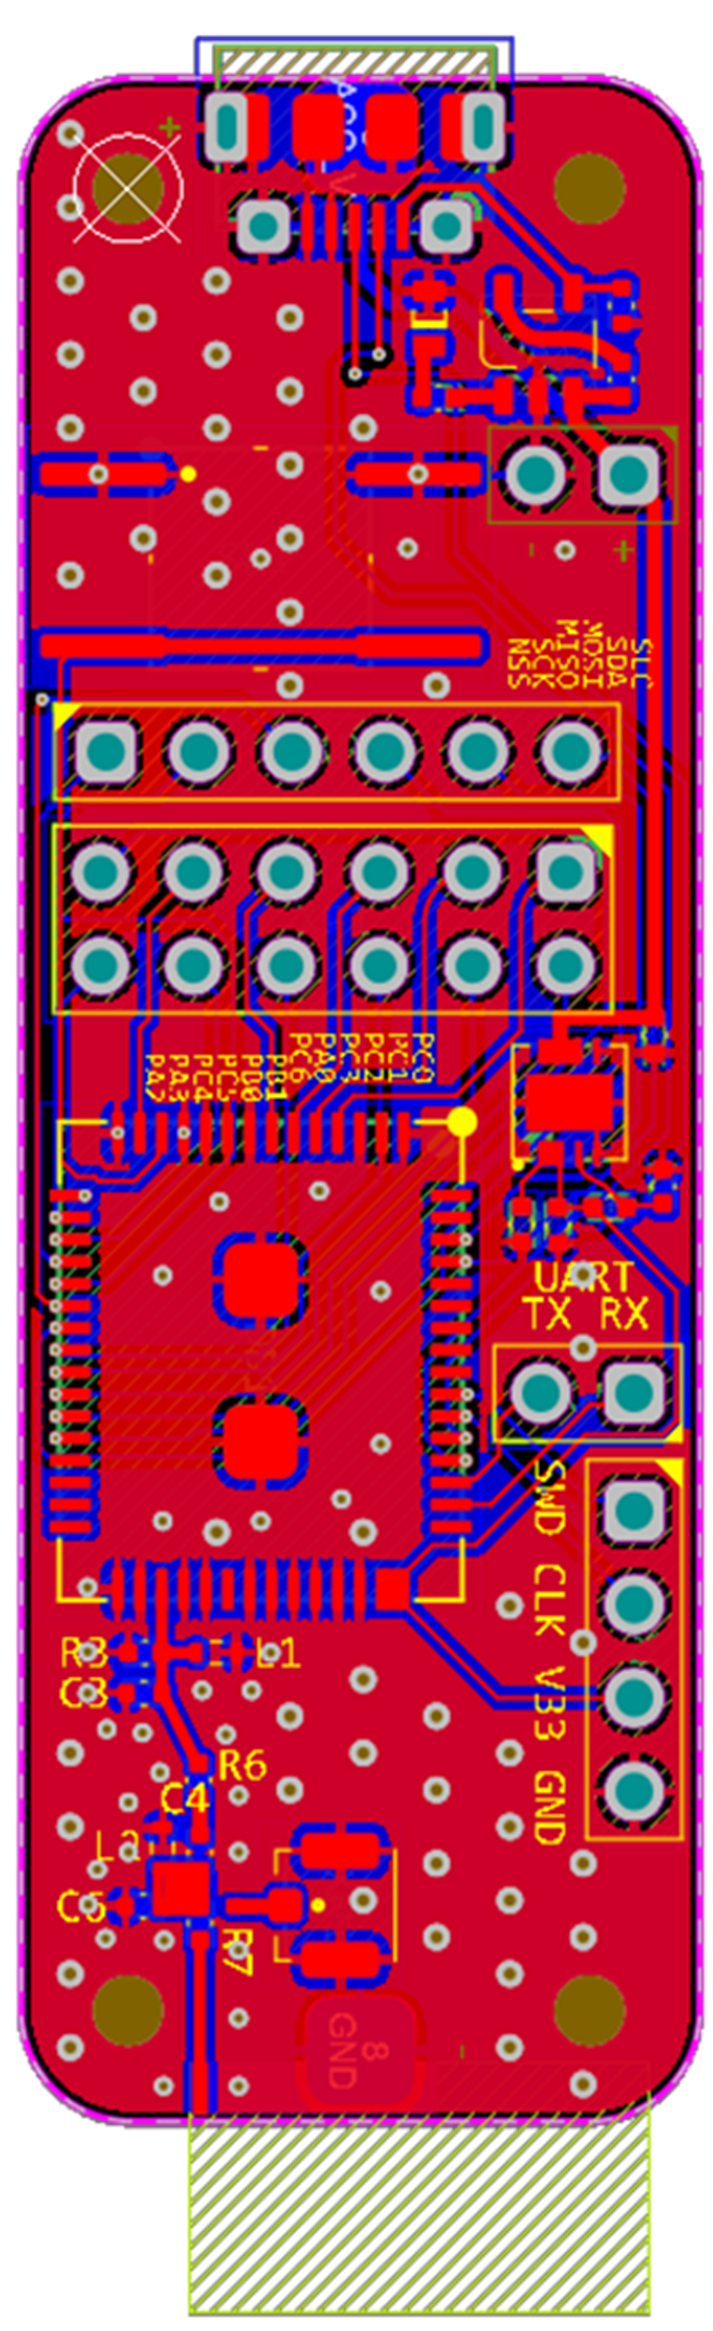
\includegraphics[height=15em]{ms-topology.png}
		\caption{}%
		\label{fig:ms-topology}
	\end{subfigure}
	\caption{%
		Два варианта исполнения платы ММ
	}%
	\label{fig:mm-topology}
\end{figure}

Первый вариант имеет размеры (ШхД) 4х4 см, а второй – 1,2х5,6 см. Заштрихованный блок представляет границы модели предполагаемой антенны. Также предусмотрена возможность подключения антенн к разъёму U.FL и установки чип-антенн.

\begin{figure}[H]
	\centering
	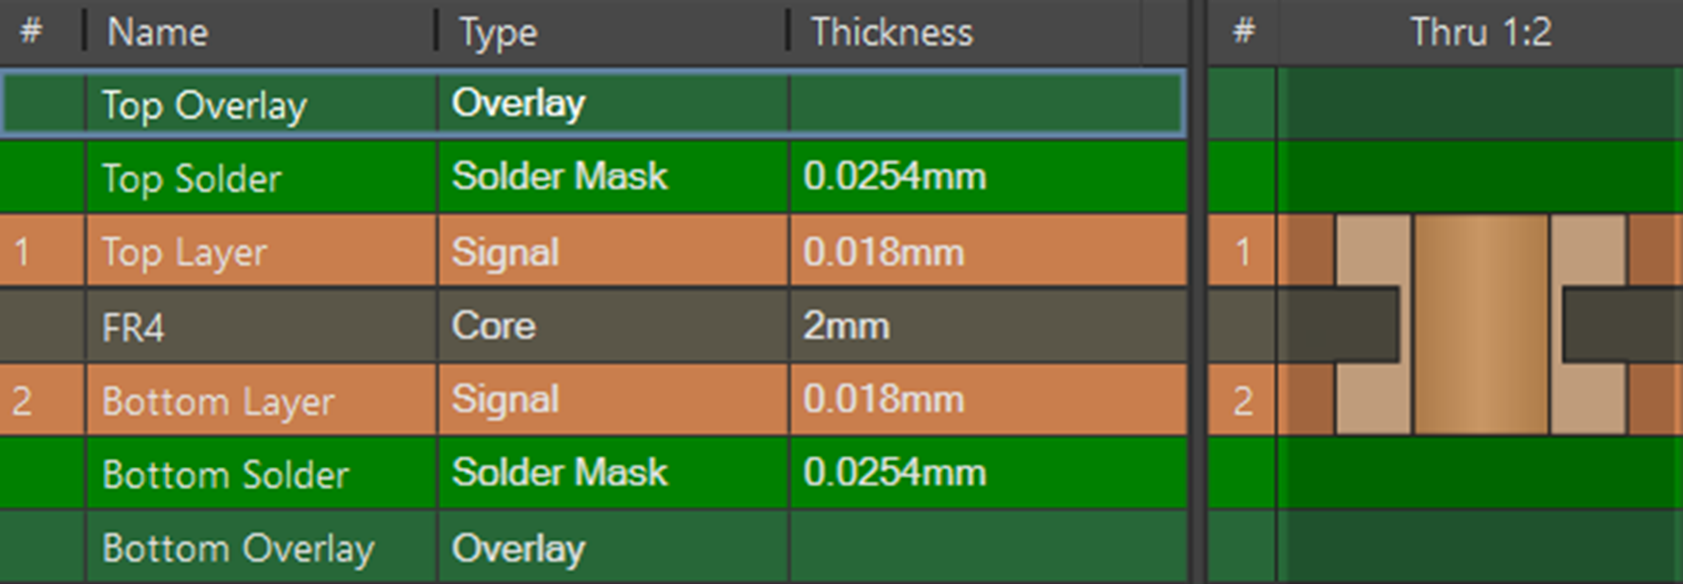
\includegraphics[width=0.7\textwidth,keepaspectratio]{mm-stackup.png}
	\caption{Cтек печатной платы МОУ}
	\label{fig:mm-stackup}
\end{figure}

\begin{figure}[H]
	\centering
	\begin{subfigure}[c]{0.3\textwidth}
		\centering
		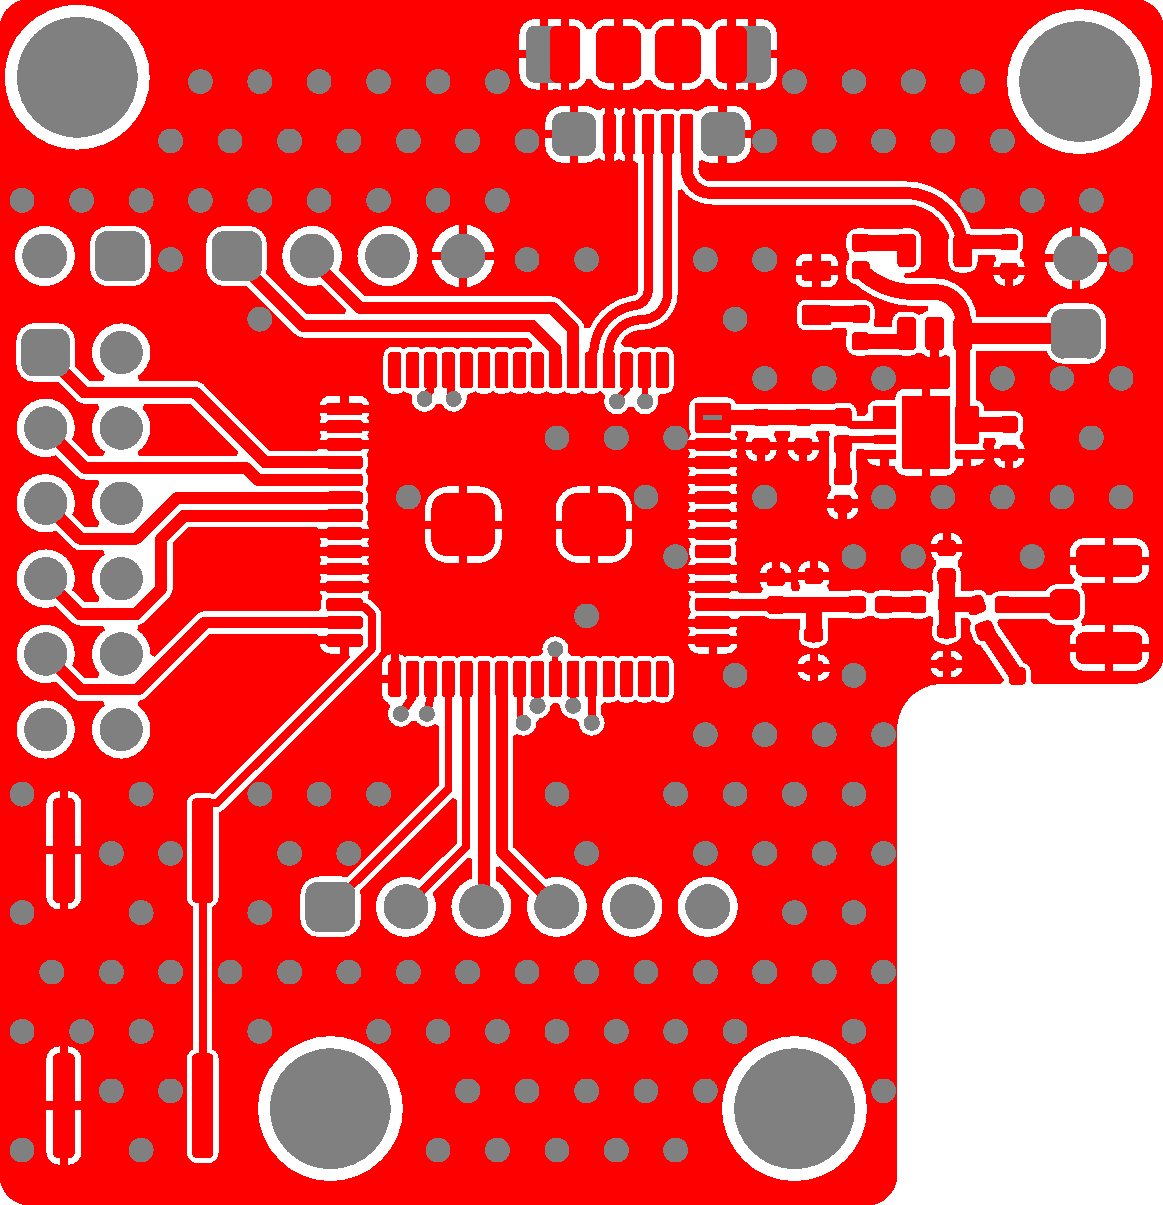
\includegraphics[width=\textwidth, keepaspectratio]{MB-Top Layer.pdf}
		\caption{}%
		\label{fig:MB-TopLayer}
	\end{subfigure}
	\hfil
	\begin{subfigure}[c]{0.3\textwidth}
		\centering
		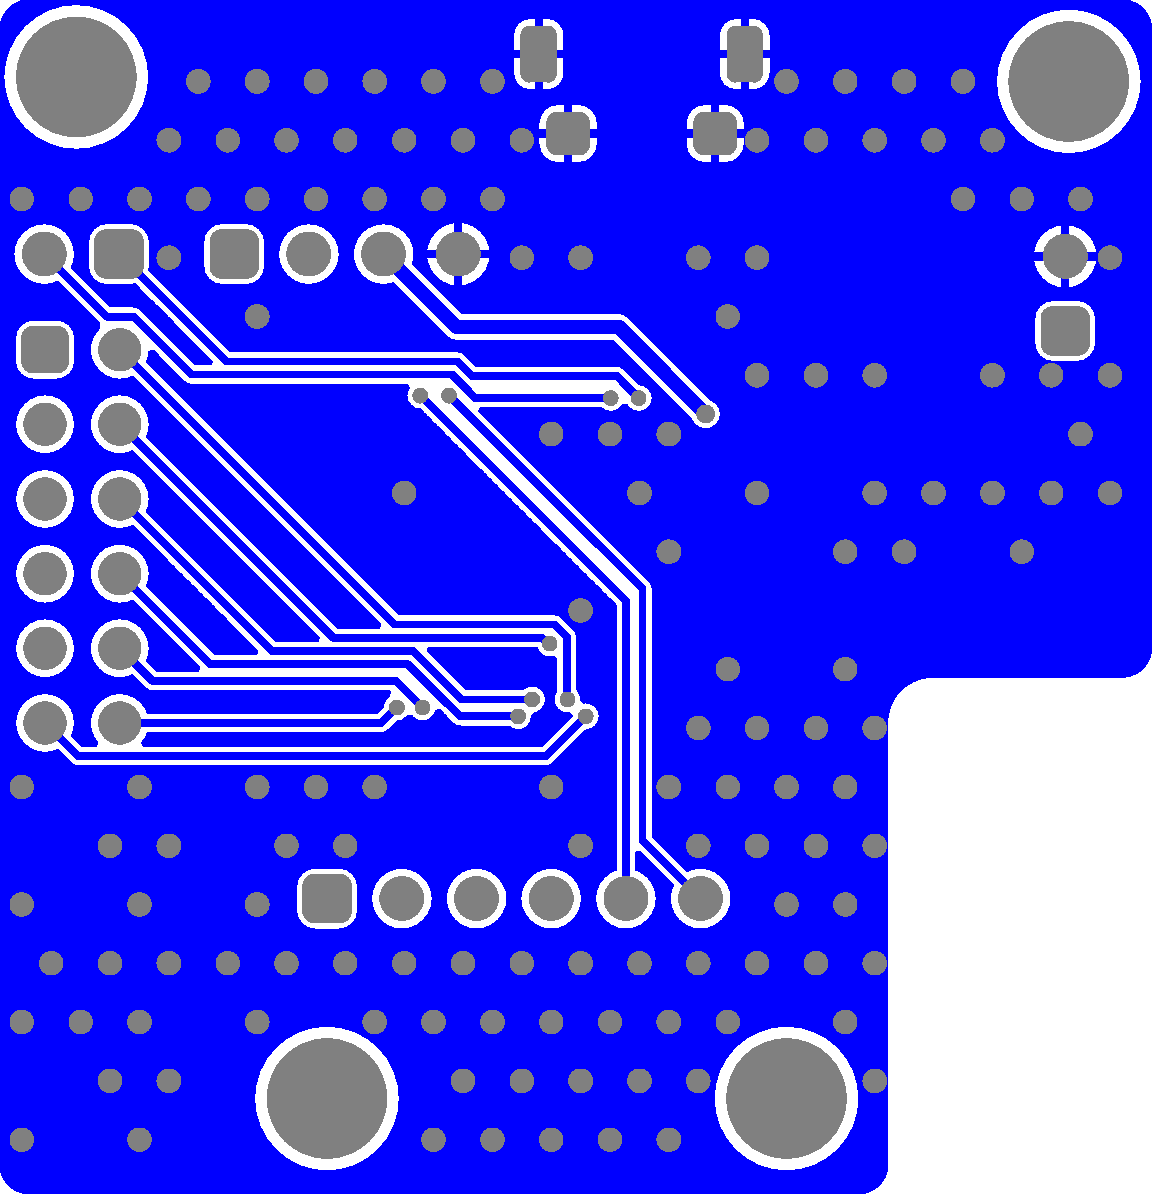
\includegraphics[width=\textwidth, keepaspectratio]{MB-Bottom Layer.pdf}
		\caption{}%
		\label{fig:MB-BottomLayer}
	\end{subfigure}
	\hfil
	\begin{subfigure}[c]{0.3\textwidth}
		\centering
		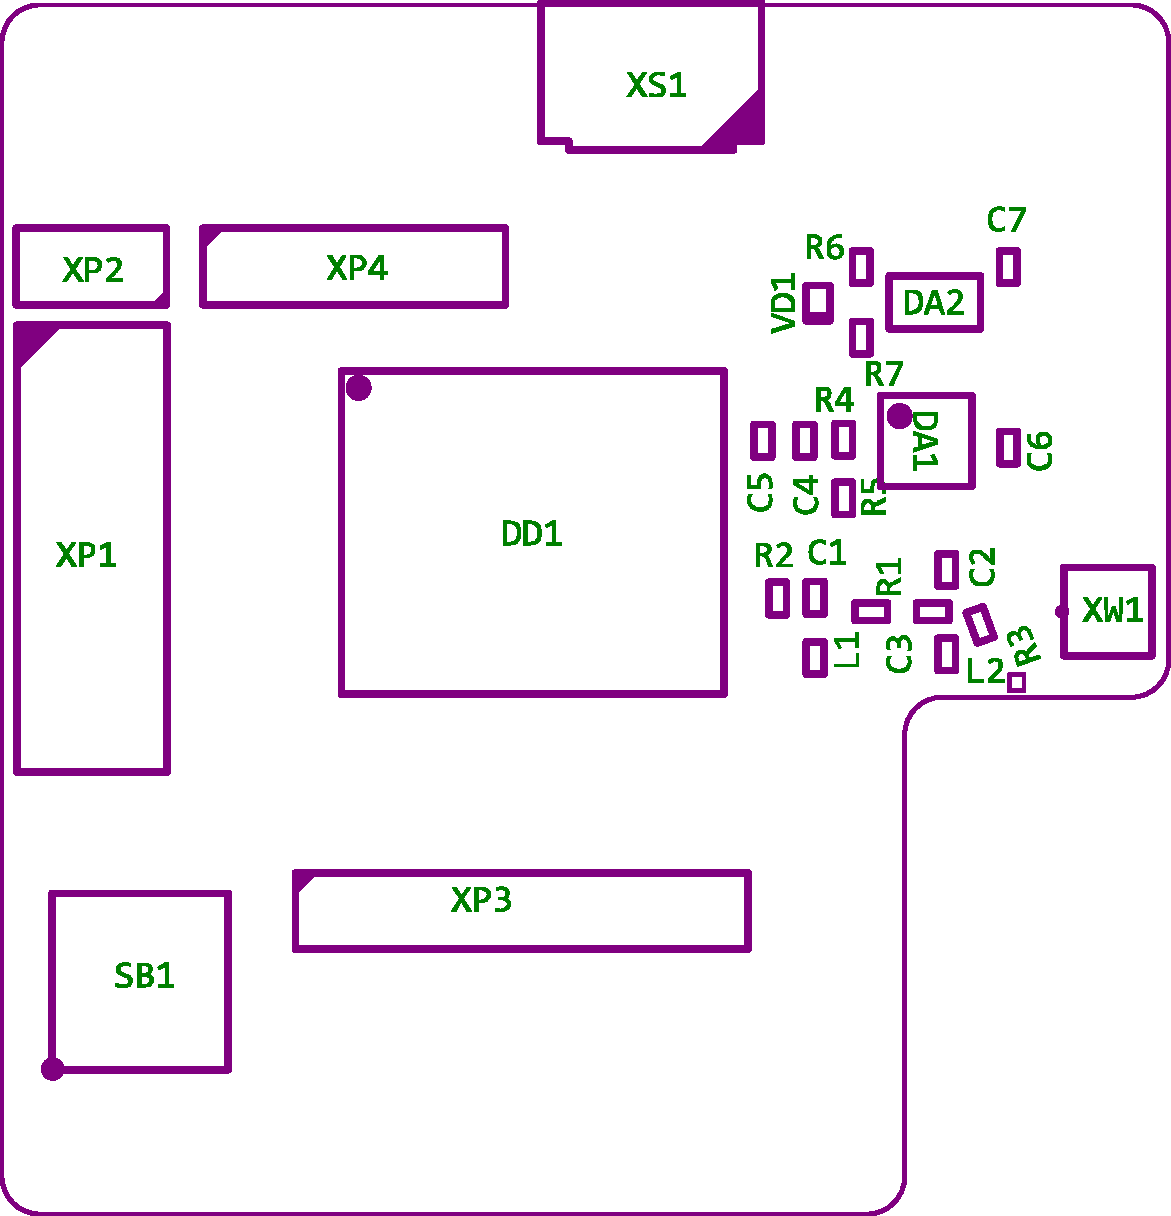
\includegraphics[width=\textwidth, keepaspectratio]{MB-Assembly Drawing.pdf}
		\caption{}%
		\label{fig:MB-AssemblyDrawing}
	\end{subfigure}
	\caption{Первый вариант исполнения. Схемы металлизации (а) верхнего и (б) нижнего слоя. (в) сборочный чертёж верхнего слоя.}
	\label{fig:mb-layers}
\end{figure}

\begin{figure}[H]
	\centering
	\begin{subfigure}[c]{0.325\textwidth}
		\centering
		\includegraphics[width=\textwidth, keepaspectratio,angle=50]{MS-Top Layer.pdf}
		\caption{}%
		\label{fig:MS-TopLayer}
	\end{subfigure}
	\hfil
	\begin{subfigure}[c]{0.325\textwidth}
		\centering
		\includegraphics[width=\textwidth, keepaspectratio,angle=50]{MS-Bottom Layer.pdf}
		\caption{}%
		\label{fig:MS-BottomLayer}
	\end{subfigure}
	\hfil
	\begin{subfigure}[c]{0.325\textwidth}
		\centering
		\includegraphics[width=\textwidth, keepaspectratio,angle=50]{MS-Assembly Drawing.pdf}
		\caption{}%
		\label{fig:MS-AssemblyDrawing}
	\end{subfigure}
	\caption{Второй вариант исполнения. Схемы металлизации (а) верхнего и (б) нижнего слоя. (в) сборочный чертёж верхнего слоя.}
	\label{fig:ms-layers}
\end{figure}


\subsection{Трёхмерная модель.}

Для сравнительной оценки размеров и демонстрации итоговых устройств приведём фотореалистичную 3D-модель из инструмента Altium Designer \linebreak Multiboard Assembly View.

\begin{figure}[H]
	\centering
	\includegraphics[width=0.7\textwidth,keepaspectratio]{mm-3d-view.png}
	\caption{трехмерные модели плат МОУ, изометрический вид.}
	\label{fig:mm-3d-view}
\end{figure}


	
	\section{Формирование документации.} \label{sect:project-docs}
	
	С использованием Altium Draftsman, TDD и инструмента создания чертежей Solidworks была сформирована документация на устройство. Вся документация выложена в открытом доступе в репозитории проекта. 
	
	\section{Разработка компактной мобильной антенны.} 

На сегодняшний день известно множество конструкций антенн, соответствующих заданным требованиям. Одними из самых распространённых и при этом простых в изготовлении являются спиральные антенны нормального излучения. Расчёт размеров антенны будем проводить с помощью LibreOffice Calc. Оригинал таблицы будет находиться в репозитории проекта, здесь же приведем лишь результаты расчёта.

\subsection{Расчёт размеров антенны.}

Антенна будет разрабатываться для частоты $f_c=\frac{864+870}{2}=867$~МГц (длина волны $\lambda\approx345$~мм)


\begin{longtblr}[
	caption = {Задаваемые параметры антенны},
	label = {table:antenna-set-params}
	]{
		colspec={Q[5,l,m]Q[3,l,m]Q[3,l,m]},
		width=0.8\textwidth,
		vlines,hlines,
		vspan=even,
		rowhead=1,
		row{1-2}={font=\bfseries}
	}
	%%%%%%%%%%%%%%%%%%%%%%%%%%%%%%%%%%%%%%%%%%%%%%%
	\SetCell[r=2]{c} Параметр & \SetCell[c=2]{c} Значение \\	
	& \SetCell[c=1]{c} Вариант 1 & \SetCell[c=1]{c}Вариант 2 \\
	%%%%%%%%%%%%%%%%%%%%%%%%%%%%%%%%%%%%%%%%%%%%%%%%
	Длина запитки $l_{feed}$ & \SetCell[c=2]{l} 3~мм \\
	Длина спирали $l_{helix}$ & \SetCell[c=2]{l} $\lambda/4-l_{feed}=83,35$~мм \\
	Диаметр проводника & \SetCell[c=2]{l} 1~мм \\
	Диаметр спирали & 5~мм & 3~мм \\
	Шаг намотки (расстояние между центрами витков) & \SetCell[c=2]{l} 1,2~мм \\
\end{longtblr}


\begin{longtblr}[
	caption = {Рассчитанные параметры антенны},
	label = {table:antenna-counted-params}
	]{
		colspec={Q[5,l,m]Q[3,l,m]Q[3,l,m]},
		width=0.8\textwidth,
		vlines,hlines,
		vspan=even,
		rowhead=1,
		row{1-2}={font=\bfseries}
	}
	%%%%%%%%%%%%%%%%%%%%%%%%%%%%%%%%%%%%%%%%%%%%%%%
	\SetCell[r=2]{c} Параметр 		& \SetCell[c=2]{c} Значение \\	
	& \SetCell[c=1]{c} Вариант 1 	& \SetCell[c=1]{c} Вариант 2 \\
	%%%%%%%%%%%%%%%%%%%%%%%%%%%%%%%%%%%%%%%%%%%%%%%%
	Высота спирали 			& \SetCell[c=1]{c} 6,35 мм 	& \SetCell[c=1]{c} 10,53 мм \\
	Число витков 			& \SetCell[c=1]{c} 5,291 	& \SetCell[c=1]{c} 8,773 \\
	Угол намотки спирали	& \SetCell[c=1]{c} $4,37^o$ & \SetCell[c=1]{c} $7,26^o$ \\
\end{longtblr}

\subsection{Моделирование антенны в CST Studio Suite.}

Для создания модели спирали использовался встроенный скрипт, для запитки — цилиндр. Все острые углы и неестественные неравномерности были сглажены. 

Для учета влияния платы была создана модель, повторяющая её контуры.

Итоговые симуляционные модели показаны на Рисунке \ref{fig:cst-model-board}.

\begin{figure}[H]
	\centering
	\begin{subfigure}[c]{0.49\textwidth}
		\centering
		\includegraphics[width=\textwidth,height=12em,keepaspectratio]{cst-model-board1.png}
		\caption{}%
		\label{}
	\end{subfigure}
	\hfill
	\begin{subfigure}[c]{0.49\textwidth}
		\centering
		\includegraphics[width=\textwidth,height=12em,keepaspectratio]{cst-model-board2.png}
		\caption{}%
		\label{}
	\end{subfigure}
	\caption{Итоговые модели для симуляции.}
	\label{fig:cst-model-board}
\end{figure}

На Рисунке \ref{fig:cst-farfield-3d} можно увидеть результаты моделирования в объемном отображении. Как видно, $K_y$ антенны равен 1.81 дБи, и излучение является тороидальным, что соответствует теории. Положение нуля зависит от длины антенны и размеров “земли”.

\begin{figure}[H]
	\centering
	\begin{subfigure}[t]{0.49\textwidth}
		\centering
		\includegraphics[width=\textwidth,height=17em,keepaspectratio]{cst-farfield-3d1.png}
		\caption{}%
		\label{}
	\end{subfigure}
	\hfill
	\begin{subfigure}[t]{0.49\textwidth}
		\centering
		\includegraphics[width=\textwidth,height=17em,keepaspectratio]{cst-farfield-3d2.png}
		\caption{}%
		\label{}
	\end{subfigure}
	\caption{Результаты моделирования поля в дальней зоне. ДН.}
	\label{fig:cst-farfield-3d}
\end{figure}

Дополнительно приведём срез диаграммы направленности (ДН) в плоскости oXZ.

\begin{figure}[H]
	\centering
	\begin{subfigure}[t]{0.49\textwidth}
		\centering
		\includegraphics[width=\textwidth,height=17em,keepaspectratio]{cst-farfield-2d1.png}
		\caption{}%
		\label{}
	\end{subfigure}
	\hfill
	\begin{subfigure}[t]{0.49\textwidth}
		\centering
		\includegraphics[width=\textwidth,height=17em,keepaspectratio]{cst-farfield-2d2.png}
		\caption{}%
		\label{}
	\end{subfigure}
	\caption{Результаты моделирования поля в дальней зоне в плоскости oXZ.}
	\label{fig:cst-farfield-2d}
\end{figure}

Исследуем поляризационную характеристику антенны. Рассмотрим графики $K_y$ антенны для вертикальной (farfield gain theta) и горизонтальной \linebreak(farfield gain phi) поляризации. 

\begin{figure}[H]
	\centering
	\begin{subfigure}[t]{0.49\textwidth}
		\centering
		\includegraphics[width=\textwidth,height=17em,keepaspectratio]{CST-antenna1-polarization1.png}
		\caption{}%
		\label{}
	\end{subfigure}
	\hfill
	\begin{subfigure}[t]{0.49\textwidth}
		\centering
		\includegraphics[width=\textwidth,height=17em,keepaspectratio]{CST-antenna1-polarization2.png}
		\caption{}%
		\label{}
	\end{subfigure}
	\caption{Поляризационная характеристика антенны. Вариант 1.}
	\label{fig:CST-antenna1-polarization}
\end{figure}

\begin{figure}[H]
	\centering
	\begin{subfigure}[t]{0.49\textwidth}
		\centering
		\includegraphics[width=\textwidth,height=17em,keepaspectratio]{CST-antenna2-polarization1.png}
		\caption{}%
		\label{}
	\end{subfigure}
	\hfill
	\begin{subfigure}[t]{0.49\textwidth}
		\centering
		\includegraphics[width=\textwidth,height=17em,keepaspectratio]{CST-antenna2-polarization2.png}
		\caption{}%
		\label{}
	\end{subfigure}
	\caption{Поляризационная характеристика антенны. Вариант 2.}
	\label{fig:CST-antenna2-polarization}
\end{figure}

Исходя из этих данных, антенна является линейно поляризованной по оси Z, и располагать её надо параллельно к антенне базовой станции (в большинстве случаев антенной базовой станции является дипольная либо монопольная антенна с аналогичной поляризационной характеристикой).

	\section{Измерение параметров устройств.}

Одним из основных параметров, влияющих на конкурентоспособность системы, является дальность связи, которую можно увеличить за счёт увеличения выходной мощности и улучшения чувствительности приемного тракта. В то же время для получения разрешения на работу изделия должны удовлетворять ограничениям на полосу частот и выходную мощность, устанавливаемым действующим законодательством. Для контроля этих параметров были разработаны следующие методики измерений.

\subsection{Средства измерений, вспомогательное оборудование и программное обеспечение.}

Для измерения параметров передаваемого сигнала потребуется анализатор спектра либо векторный анализатор цепей (ВАЦ).
Для измерения параметров приемного тракта потребуется генератор сигнала произвольной формы и анализатор спектра либо ВАЦ. 
В данной методике будет описан процесс измерения с использованием анализатора спектра Rohde\&Schwarz FSEB и генератора сигнала Rohde\&Schwarz SMU200A. 
Для автоматизации измерений все исследуемые устройства будут подключены к ПК с установленным ПО для управления СИ и терминалом последовательного порта для управления ИУ. Также потребуется специальное ПО с поддержкой AT-команд для исследуемых устройств.

\subsection{Измерение параметров выходного тракта.}

\begin{figure}[H]
	\centering
	\includegraphics[width=0.7\textwidth,keepaspectratio]{TransmitterMeasSch.pdf}
	\caption{Схема установки измерения параметров передаваемого сигнала.}
	\label{fig:TransmitterMeasSch}
\end{figure}

\subsubsection{Подготовка к проведению измерений}

\begin{enumerate}
	\setlength\itemsep{-1ex}
	\item Включить ПК 
	\item Включить анализатор спектра. Прогреть в течение 15 минут.
	\item Откалибровать анализатор спектра
	\begin{enumerate}
		\item Открыть меню калибровки нажав кнопку CAL в разделе SYSTEM
		\item Запустить процесс калибровки, выбрав пункт SHORT CAL.
		\item Дождаться окончания процесса калибровки
	\end{enumerate}
\end{enumerate}

\subsubsection{Выполнение измерений}

\begin{enumerate}
	\setlength\itemsep{-1ex}
	\item Включить исследуемое устройство и подключить его к ПК.
	\item Запустить терминал. 
	\item Отправить на ИУ AT-команды
		\begin{enumerate}
			\setlength\itemsep{-1ex}
			\item AT+TCONF=868900000:14:1:7:4/5 (установить частоту 868,9 МГц, мощность 14 дБм, полосу 125кГц, SF=7, CR=4/5)
			\item AT+TTX=5 (отправить 5 пакетов)
		\end{enumerate}
	\item Установить на анализаторе спектра центральную частоту 867 МГц и диапазон частот 10 МГц. Наблюдать спектрограмму.
		\begin{figure}[H]
			\centering
			\includegraphics[width=0.7\textwidth,keepaspectratio]{out-power-meas-ex.png}
			\caption{Схема установки измерения параметров передаваемого сигнала.}
			\label{fig:out-power-meas-ex}
		\end{figure}
	\item Установить следующую частоту командой AT+TCONF=86900000:14:1:7:⅘
	\item Наблюдать спектрограмму.
	\item Повторить пункты 3-6 для других частот и амплитуд.
	\item Для измерения уровня мощности на гармониках передаваемого сигнала установим диапазон измерений от 100 МГц до 6 ГГц
		\begin{figure}[H]
			\centering
			\includegraphics[width=0.6\textwidth,keepaspectratio]{out-harm-meas-ex.png}
			\caption{Схема установки измерения параметров передаваемого сигнала.}
			\label{fig:out-harm-meas-ex}
		\end{figure}	
\end{enumerate}

\subsection{Измерение параметров выходного тракта.}

\begin{figure}[H]
	\centering
	\includegraphics[width=0.6\textwidth,keepaspectratio]{RecieverMeasSch.pdf}
	\caption{Схема установки измерения чувствительности приемника.}
	\label{fig:RecieverMeasSch}
\end{figure}

\subsubsection{Подготовка к проведению измерений}

\begin{enumerate}
	\setlength\itemsep{-1ex}
	\item Включить ПК 
	\item Включить анализатор спектра и генератор. Прогреть в течение 15 минут.
	\item Откалибровать анализатор спектра
	\begin{enumerate}
		\item Открыть меню калибровки нажав кнопку CAL в разделе SYSTEM
		\item Запустить процесс калибровки, выбрав пункт SHORT CAL.
		\item Дождаться окончания процесса калибровки
	\end{enumerate}
\end{enumerate}

\subsubsection{Выполнение измерений для одного канала.}

\begin{enumerate}
	\setlength\itemsep{-1ex}
	\item Загрузить в генератор файл модулирующего сигнала и установить частоту дискретизации равной 4 ширинам полосы канала. Для 125 кГц канала требуется частота дискретизации 500 кГц. Для полосы 250 кГц, соответственно, 1 МГц.
	\item Включить генерацию центральной частоты и модуляцию.
	\item Включить исследуемое устройство и подключить его к ПК.
	\item Запустить терминал. 
	\item Отправить на ИУ AT-команды
	\begin{enumerate}
		\setlength\itemsep{-1ex}
		\item AT+TCONF=868900000:14:1:7:4/5 (установить частоту 868,9 МГц, мощность 14 дБм, полосу 125кГц, SF=7, CR=4/5)
		\item AT+TRX=50 (ожидать приём 50 пакетов)
	\end{enumerate}
	\item Дождаться возвращения в терминал вычисленного процента пакетной ошибки. 
	\item Если процент ошибок менее 1\% – уменьшить мощность генерируемого сигнала на 1 дБ.
	\item Повторять пункты 5 и 6 до тех пор, пока количество ошибок не превысит 1\%. Уровень мощности генерируемого сигнала будем считать первым значением чувствительности. 
	\item Продолжать исследование до тех пор, пока количество ошибок не превысит 15\%. Уровень мощности генерируемого сигнала будем считать вторым значением чувствительности. 
	
\end{enumerate}

\subsubsection{Выполнение измерений для двух каналов.}

\begin{enumerate}
	\item Загрузить в генератор 1 файл модулирующего сигнала (SF=7, CR=4/5, W=125 кГц) и установить частоту дискретизации равной 500 кГц. 
	\item Загрузить в генератор 1 файл модулирующего сигнала (SF=7, CR=4/5, W=250 кГц) и установить частоту дискретизации равной 1000 кГц. 
	\item Включить генерацию центральной частоты и модуляцию на обоих генераторах.
	\item Включить исследуемое устройство и подключить его к ПК.
	\item Запустить терминал. 
	\item Отправить на ИУ AT-команды
	\begin{enumerate}
		\item AT+TCONF=868900000:14:1:7:4/5:1 (установить частоту 868,9  МГц, мощность 14 дБм, полосу 125 кГц, SF=7, CR=4/5, фильтр 1)
		\item AT+TCONF=868900000:14:2:7:4/5:2 (установить частоту 868,9 МГц, мощность 14 дБм, полосу 250 кГц, SF=7, CR=4/5, фильтр 2)
		\item AT+TRX=50 (ожидать приём 50 пакетов)
	\end{enumerate}
	\item Дождаться возвращения в терминал вычисленного процента пакетной ошибки. 
	\item Если процент ошибок менее 1\% – уменьшить мощность генерируемого сигнала на 1 дБ.
	\item Повторять пункты 5 и 6 до тех пор, пока количество пакетных ошибок одного из каналов не превысит 1\%. Уровень мощности генерируемого сигнала будем считать первым значением чувствительности по данному каналу.
	\item Продолжать уменьшать мощность второго канала до тех пока, пока количество ошибок  не превысит 1\%.
	\item Продолжать исследование обоих каналов для 15\% уровня пакетных ошибок. Уровень мощности генерируемого сигнала будем считать вторым значением чувствительности. 
\end{enumerate}
















	\section{Расчёт дальности связи.}

Используя данные моделирования, полученные в предыдущих главах, произведём оценочный расчёт дальности связи разрабатываемой системы. Структурная схема исследуемой модели показана на Рисунке \ref{fig:System-StructSch}

\begin{figure}[H]
	\centering
	\includegraphics[width=\textwidth,keepaspectratio]{System-StructSch.pdf}
	\caption{ Структурная схема исследуемой системы}%
	\label{fig:System-StructSch}
\end{figure}

Дано:

\begin{itemize}
	\setlength\itemsep{-1ex}
	\item Усиление антенны БС – 13 дБи
	\item Усиление антенны МОУ – 2 дБи
	\item Выходная мощность – 14 дБм
	\item Чувствительность (худш) – -128 дБм
	\begin{itemize}
		\setlength\itemsep{-1ex}
		\item Бюджет канала (мин) – 142 дБ
	\end{itemize}
	\item Чувствительность (лучш) – -140 дБм
	\begin{itemize}
		\setlength\itemsep{-1ex}
		\item Бюджет канала (макс) – 154 дБ
	\end{itemize}	
\end{itemize}

Максимальная и минимальная чувствительность определяются для максимальной (11 Кб/с, SF=7) и минимальной (0.3 Кб/с, SF=12) скорости передачи данных. 

Для проведения виртуального эксперимента будем использовать модель Окамуры-Хата. Данная модель описывает процесс распространения (затухания) радиоволн в урбанизированных районах без учета информации о рельефе местности и адаптирована для расчета мобильных сетей связи. Модель Окамура-Хата предназначена для РЭС, используемых в диапазоне от 150(100) до 1 500 МГц. Модель Окамура-Хата учитывает особенности территории, застройки (городская, пригородная, открытая сельская) и населенного пункта (большой, средний, маленький).

Задача --- уложиться в предоставляемый бюджет канала. Предполагаемая высота подвеса антенны БС -- 40 м. Исследуемые высоты подвеса антенны модуля IoT -- 1-15 м. Модель потерь в городских условиях формируется следующим образом:

\begin{equation*}
	\centering
	L_U \; = \; 69.55 \; + \; 26.16 \; \lg f \; - \; 13.82 \; \lg h_B \; - \; C_H \; + \; [44.9 \; - \; 6.55 \; \lg h_B] \; \lg d
\end{equation*}

Где для небольших и средних городов:

\begin{equation*}
	\centering
	C_H \; = \; 0.8 \; + \; (\; 1.1 \; \lg f \; - \; 0.7 \; ) \; h_M \; - \; 1.56 \; \lg f 
\end{equation*}

И для больших:

\begin{equation*}
	\centering
	C_H \; = \begin{cases}\;8.29 \; (\; \lg ({1.54 h_M}))^2 \; - \; 1.1 \; \mbox{  , if } 150 \le f \le 200 \\ \; 3.2 \; (\lg ({11.75 h_M}))^2 \; - \; 4.97 \; \mbox{ , if }200 < f \le 1500 \end{cases}
\end{equation*}

Здесь:
$L_U$ — потери в городских условиях, дБ
$h_B$ — высота подвеса базовой антенны
$h_M$ — высота подвеса мобильной антенны
$f$ — частота передачи
$C_H$ — коэффициент коррекции антенны
$d$  — дистанция связи

Потери в условиях пригорода рассчитываются по формуле:

\begin{equation*}
	\centering
	L_{SU}\; = \; L_U \; - \; 2 \big( \lg {\frac{f}{28}}\big)^2 \; - \;5.4 
\end{equation*}

И, наконец, в открытых условиях:

\begin{equation*}
	\centering
	L_{O}\; = \; L_U \; - \; 4.78 \big( \lg {f}\big)^2 \; + \; 18.33 \big( \lg {f}\big)- \;40.94
\end{equation*}
 
Расчеты будем вести в MATLAB. Листинг кода представлен в Приложении A. 

Результаты расчёта показаны на Рисунках \ref{fig:system-count-city} и \ref{fig:system-count-suburb}. Ось oY показывает уровень потерь, ось oX показывает расстояние между устройствами. Горизонтальная черта показывает уровень потерь, при превышении которого количество ошибок будет превышать 1\%.


\begin{figure}[H]
	\centering
	\includegraphics[width=\textwidth,keepaspectratio]{system-count-city.pdf}
	\caption{Результаты расчёта дальности связи в условиях плотной городской застройки.}
	\label{fig:system-count-city}
\end{figure}

\begin{figure}[H]
\centering
\includegraphics[width=\textwidth,keepaspectratio]{system-count-suburb.pdf}
\caption{Результаты расчёта дальности связи в условиях пригорода и сельской местности.}
\label{fig:system-count-suburb}
\end{figure}

Проведённые расчеты позволяют приблизительно оценить структуру сети, а следовательно проводить предварительные экономические расчеты.





	\ssect{Заключение}

В данной работе были разработаны подсистема связи для базовых станций LoRa и мобильное оконечное устройство, удовлетворяющие требованиям технического задания (ТЗ приведено в Главе \ref{sect:task}). Также для мобильного модуля были разработаны модели компактной антенны. В конце был проведен оценочный расчёт возможностей системы. Для проверки соответствия разработанных устройств техническому заданию были разработаны методики проверки параметров  приемного и передающего трактов. 

Разработка относится к проектам с открытой архитектурой (исходные файлы выложены в репозитории проекта по адресу \url{https://github.com/lazbaphilipp/diploma-barchelor}) и распространяется по лицензии MIT, а следовательно, может использоваться в качестве основы для других открытых и закрытых проектов в данной и смежной областях	
	\nocite{*}
\printbibliography[title={Список использованных источников},heading=bibintoc]
	\ssect{Приложение А. Листинг кода программы расчёта дальности связи.}

\definecolor{codegreen}{rgb}{0,0.6,0}
\definecolor{codegray}{rgb}{0.5,0.5,0.5}
\definecolor{codepurple}{rgb}{0.58,0,0.82}
\definecolor{backcolour}{rgb}{0.95,0.95,0.92}
\definecolor{mygreen}{rgb}{0,0.6,0}
\definecolor{mygray}{rgb}{0.5,0.5,0.5}
\definecolor{mymauve}{rgb}{0.58,0,0.82}

\lstset{ 
	backgroundcolor=\color{white},   % choose the background color; you must add \usepackage{color} or \usepackage{xcolor}; should come as last argument
	basicstyle=\footnotesize,        % the size of the fonts that are used for the code
	breakatwhitespace=false,         % sets if automatic breaks should only happen at whitespace
	breaklines=true,                 % sets automatic line breaking
	captionpos=b,                    % sets the caption-position to bottom
	commentstyle=\color{mygreen},    % comment style
	deletekeywords={...},            % if you want to delete keywords from the given language
	escapeinside={\%*}{*)},          % if you want to add LaTeX within your code
	extendedchars=true,              % lets you use non-ASCII characters; for 8-bits encodings only, does not work with UTF-8
	firstnumber=000,                % start line enumeration with line 1000
	frame=single,	                   % adds a frame around the code
	keepspaces=true,                 % keeps spaces in text, useful for keeping indentation of code (possibly needs columns=flexible)
	keywordstyle=\color{blue},       % keyword style
	language=Matlab,                 % the language of the code
	morekeywords={*,...},            % if you want to add more keywords to the set
	numbers=left,                    % where to put the line-numbers; possible values are (none, left, right)
	numbersep=5pt,                   % how far the line-numbers are from the code
	numberstyle=\tiny\color{mygray}, % the style that is used for the line-numbers
	rulecolor=\color{black},         % if not set, the frame-color may be changed on line-breaks within not-black text (e.g. comments (green here))
	showspaces=false,                % show spaces everywhere adding particular underscores; it overrides 'showstringspaces'
	showstringspaces=false,          % underline spaces within strings only
	showtabs=false,                  % show tabs within strings adding particular underscores
	stepnumber=1,                    % the step between two line-numbers. If it's 1, each line will be numbered
	stringstyle=\color{mymauve},     % string literal style
	tabsize=2,	                   % sets default tabsize to 2 spaces
	title=\lstname                   % show the filename of files included with \lstinputlisting; also try caption instead of title
}

\lstinputlisting[language=Matlab]{Project/SystemCount.m}
	
\end{document}